% !TeX root = ./main.tex

%% ========================================================================
%%%% Basic settings
%% ========================================================================
%% (idea of using newcommands for basic documentclass settings from: Thomas Schlager)

\newcommand{\mypapersize}{A4}
%% e.g., "A4", "letter", "legal", "executive", ...
%% The size of the paper of the resulting PDF file.

\newcommand{\mylaterality}{oneside}
%% "oneside" or "twoside"
%% Either you are creating a document which is printed on both, left pages
%% and right pages (twoside) or you create a document which is printed
%% on right pages only (oneside).

\newcommand{\mydraft}{false}
%% "true" or "false"
%% Use draft mode? If true, included graphics are replaced by empty
%% rectangles (of same size) and overfull boxes (in margin space) are
%% marked with black box (-> easy to spot!)

\newcommand{\myparskip}{half}
%% e.g., "no", "full", "half", ...
%% How to separate paragraphs: indention ("no") or spacing ("half",
%% "full", ...).

\newcommand{\myBCOR}{0mm}
%% Inner binding correction. This value depends on the method which is
%% being used to bind your printed result. Some techniques do not
%% require a binding correction at all ("0mm"), other require for
%% example "5mm". Refer to KOMA script documentation for a detailed
%% explanation what a binding correction is and how to measure it.

\newcommand{\myfontsize}{12pt}
%% e.g., 10pt, 11pt, 12pt
%% The font size of the main text in pt (points).

\newcommand{\mylinespread}{1.0}
%% e.g., 1.0, 1.5, 2.0
%% Line spacing in %/100. For example 1.5 means 150% of the usual line
%% spacing. Please use with caution: 100% ("1.0") is fine because the
%% font was designed for it.

\newcommand{\mylanguage}{english,ngerman}
\newcommand{\mycitelanguage}{ngerman}

%% "english,ngerman", "ngerman,english", ...
%% NOTE: The *last* language is the active one!
%% See babel documentation for further details.

%% BibLaTeX-settings: (see biblatex reference for further description)
\newcommand{\mybiblatexstyle}{authoryear-comp}
%% e.g., "alphabetic", "authoryear", ...
%% The biblatex style which is being used for referencing. See
%% biblatex documentation for further details and more values.
%%
%% CAUTION: if you change the style, please check for (in)compatible
%%          "biblatex" package options in the file
%%          "template/preamble.tex"! For example: "alphabetic" does
%%          not have an option "dashed=..." and causes an error if it
%%          does not get removed from the list of options.

\newcommand{\mybiblatexdashed}{false}  %% "true" or "false"
%% If true: replace recurring reference authors with a dash.

\newcommand{\mybiblatexbackref}{true}  %% "true" or "false"
%% If true: create backward links from reference to citations.

\newcommand{\mybiblatexfile}{references.bib}
\newcommand{\mybiblatexfileA}{project-A-virenmonitoring/references.bib}
\newcommand{\mybiblatexfileU}{project-U-wintersterblichkeit/references.bib}
\newcommand{\mybiblatexfileV}{project-V-virendiagnostik/references.bib}

%% Name of the biblatex file that holds the references.

\newcommand{\mydispositioncolor}{30,103,182}
%% e.g., "30,103,182" (blue/turquois), "0,0,0" (black), ...
%% Color of the headings and so forth in RGB (red,green,blue) values.
%% NOTE: if you are using "0,0,0" for black, printers might still
%%       recognize pages as color pages. In case this is a problem
%%       (paying for color print-outs vs. paying for b/w-printouts)
%%       please edit file "template/preamble.tex" and change
%%       "\definecolor{DispositionColor}{RGB}{\mydispositioncolor}"
%%       to "\definecolor{DispositionColor}{gray}{0}" and thus
%%       overwriting the value of \mydispositioncolor above.

\newcommand{\mycolorlinks}{true}  %% "true" or "false"
%% Enables or disables colored links (hyperref package).

\newcommand{\mytitlepage}{frontpages/title.tex}

\newcommand{\mytodonotesoptions}{}
%% e.g., "" (empty), "disable", ...
%% Options for the todonotes-package. If "disable", all todonotes will
%% be hidden (including listoftodos).

%% Load main settings for document preamble:
\documentclass[%
fontsize=\myfontsize,%% size of the main text
paper=\mypapersize,  %% paper format
parskip=\myparskip,  %% vertical space between paragraphs (instead of indenting first par-line)
DIV=16,            %% calculates a good DIV value for type area; 66 characters/line is great
headinclude=true,    %% is header part of margin space or part of page content?
headings=optiontoheadandtoc,
footinclude=false,   %% is footer part of margin space or part of page content?
open=right,          %% "right" or "left": start new chapter on right or left page
appendixprefix=true, %% adds appendix prefix; only for book-classes with \backmatter
bibliography=totoc,  %% adds the bibliography to table of contents (without number)
draft=\mydraft,      %% if true: included graphics are omitted and black boxes
                     %%          mark overfull boxes in margin space
BCOR=\myBCOR,        %% binding correction (depends on how you bind
                     %% the resulting printout.
\mylaterality       %% oneside: document is not printed on left and right sides, only right side
                     %% twoside: document is printed on left and right sides
]{scrbook}  %% article class of KOMA: "scrartcl", "scrreprt", or "scrbook".
            %% CAUTION: If documentclass will be changed, *many* other things
            %%          change as well like heading structure, ...

% FIXXME: adopting class usage:
% from scrbook -> scrartcl OR scrreport:
% - remove appendixprefix from class options
% - remove \frontmatter \mainmatter \backmatter \appendix from main.tex

% FIXXME: adopting language:
% add or modify language parameter of package »babel« and use language switches described in babel-documentation

%doc%
%doc% \subsection{\texttt{inputenc}: UTF8 as input charset}
%doc%
%doc% You are able and should use \myacro{UTF8} character settings for writing these \TeX{}-files.
%doc%
%\usepackage{ucs}             %% UTF8 as input characters; UCS incompatible to biblatex
\usepackage[T1]{fontenc} %% for special characters
\usepackage[utf8]{inputenc} %% UTF8 as input characters

%% Source: http://latex.tugraz.at/latex/tutorial#laden_von_paketen

%doc%
%doc% \subsection{\texttt{textcomp}: Support for Text Companion fonts}
%doc%
%doc% Provides some text symbols such as bullet in \myacro{TS1} encoding.
%doc% Depending on what font or symbols you use, you might not even need this.
%doc% Removing this package will at worst result in a warning.
\usepackage{textcomp}
%% Source: https://www.ctan.org/pkg/textcomp

%doc%
%doc% \subsection{\texttt{babel}: Language settings}
%doc%
%doc% The default setting of the language is American. Please change settings for
%doc% additional or alternative languages used in \texttt{main.tex}.
%doc%
%doc% Please note that the default language of the document is the \emph{last} language
%doc% which is added to the package options.
%doc%
%doc% To set only parts of your document in a different language as the rest, use for example\newline
%doc% \verb+\foreignlanguage{ngerman}{Beispieltext in deutscher Sprache}+\newline
%doc% For using foreign language quotes, please refer to the \verb+\foreignquote+,
%doc% \verb+\foreigntextquote+, or \verb+\foreignblockquote+ provided by
%doc% \texttt{csquotes} (see Section~\ref{sub:csquotes}).
%doc%
\usepackage[\mylanguage]{babel}  %% used languages; default language is *last* language of options

%% improved german hyphen breaks
\usepackage[ngerman=ngerman-x-latest]{hyphsubst}

% allow breaks after "-" in URLs
\usepackage[hyphens]{url}


%doc%
%doc% \subsection{\texttt{scrlayer-scrpage}: Headers and footers}
%doc%
%doc% Since this template is based on \myacro{KOMA} script it uses its great
%doc% \texttt{scrlayer-scrpage} (previously \texttt{scrpage2})
%doc% package for defining header and footer information. Please refer to the \myacro{KOMA}
%doc% script documentation how to use this package.
%doc%
\usepackage{scrlayer-scrpage} %%  advanced page style using KOMA


%doc% \subsubsection{Example citation commands}
%doc%
%doc% This section demonstrates some example citations using the style \texttt{authoryear}.
%doc% You can change the citation style in \texttt{main.tex} (\texttt{mybiblatexstyle}).
%doc%
%doc% \begin{itemize}
%doc% \item cite \cite{Eijkhout2008} and cite \cite{Bringhurst1993, Eijkhout2008}.
%doc% \item citet \citet{Eijkhout2008} and citet \citet{Bringhurst1993, Eijkhout2008}.
%doc% \item autocite \autocite{Eijkhout2008} and autocite \autocite{Bringhurst1993, Eijkhout2008}.
%doc% \item autocites \autocites{Eijkhout2008} and autocites \autocites{Bringhurst1993, Eijkhout2008}.
%doc% \item citeauthor \citeauthor{Eijkhout2008} and citeauthor \citeauthor{Bringhurst1993, Eijkhout2008}.
%doc% \item citetitle \citetitle{Eijkhout2008} and citetitle \citetitle{Bringhurst1993, Eijkhout2008}.
%doc% \item citeyear \citeyear{Eijkhout2008} and citeyear \citeyear{Bringhurst1993, Eijkhout2008}.
%doc% \item textcite \textcite{Eijkhout2008} and textcite \textcite{Bringhurst1993, Eijkhout2008}.
%doc% \item smartcite \smartcite{Eijkhout2008} and smartcite \smartcite{Bringhurst1993, Eijkhout2008}.
%doc% \item footcite \footcite{Eijkhout2008} and footcite \footcite{Bringhurst1993, Eijkhout2008}.
%doc% \item footcite with page \footcite[p.42]{Eijkhout2008} and footcite with page \footcite[compare][p.\,42]{Eijkhout2008}.
%doc% \item fullcite \fullcite{Eijkhout2008} and fullcite \fullcite{Bringhurst1993, Eijkhout2008}.
%doc% \end{itemize}
%doc%
%doc% Please note that the citation style as well as the bibliography style
%doc% can be changed very easily. Refer to the settings in
%doc% \texttt{main.tex} as well as the very good documentation of \texttt{biblatex}.
%doc%

%doc% \subsubsection{Using this template with \myacro{APA} style}
%doc%
%doc% First, you have to have the \myacro{APA} biblatex style
%doc% installed. Modern \LaTeX{} distributions do come with
%doc% \texttt{biblatex} and \myacro{APA} style. If so, you will find the
%doc% files \texttt{biblatex-apa.pdf} (style documentation) and
%doc% \texttt{biblatex-apa-test.pdf} (file with citation examples) on your
%doc% hard disk.
%doc%
%doc% \begin{enumerate}
%doc% \item Change the style according to \verb#\newcommand{\mybiblatexstyle}{apa}#
%doc% \item Add \verb#\DeclareLanguageMapping{american}{american-apa}# or \\
%doc%   \verb#\DeclareLanguageMapping{german}{german-apa}# to your
%doc%   preamble\footnote{You might want to use section \enquote{MISC
%doc%       self-defined commands and settings} for this.}
%doc% \end{enumerate}
%doc%
%doc% These steps change the biblatex style to \myacro{APA} style

%doc%
%doc% \subsubsection{Using this template with \textsc{Bib}\TeX{}}
%doc%
%doc% If you do not want to use \texttt{Biber} and \texttt{biblatex}, you
%doc% have to change several things:
%doc% \begin{itemize}
%doc% \item in \verb#preamble/preamble.tex#
%doc%   \begin{itemize}
%doc%   \item remove the usepackage command of \texttt{biblatex}
%doc%   \item remove the \verb#\addbibresource{...}# command
%doc%   \end{itemize}
%doc% \item in \verb#main.tex#
%doc%   \begin{itemize}
%doc%   \item replace \verb=\printbibliography= with the usual
%doc%     \verb=\bibliographystyle{yourstyle}= and \verb=\bibliography{yourbibfile}=
%doc%   \end{itemize}
%doc% \item if you are using \myacro{GNU} \texttt{make}: modify \verb=Makefile=
%doc%   \begin{itemize}
%doc%   \item replace \verb#BIBTEX_CMD = biber# with \verb#BIBTEX_CMD = bibtex#
%doc%   \end{itemize}
%doc% \item Use the reference file \texttt{references-bibtex.bib}
%doc%   instead of \texttt{references-biblatex.bib}
%doc% \end{itemize}
%doc%
%doc%
\usepackage[backend=biber, %% using "biber" to compile references (instead of "biblatex")
style=\mybiblatexstyle, %% see biblatex documentation
%style=alphabetic, %% see biblatex documentation
dashed=\mybiblatexdashed, %% do *not* replace recurring reference authors with a dash
backref=\mybiblatexbackref, %% create backlings from references to citations
uniquelist=false,
natbib=true, %% offering natbib-compatible commands
maxcitenames=2,
hyperref=true, %% using hyperref-package references
date=year,
sorting=ynt, sortcites %% sort multiple cites by date
]{biblatex}  %% remove, if using BibTeX instead of biblatex

\DefineBibliographyStrings{ngerman}{andothers={et\ al\adddot}} % aus u.a. zu et al. machen

%doc%
%doc% \subsection{Miscellaneous packages} \label{subsec:miscpackages}
%doc%
%doc% There are several packages included by default. You might want to activate or
%doc% deactivate them according to your requirements:
%doc%
%doc% \begin{enumerate}

%doc% \item[\texttt{\href{http://www.ctan.org/pkg/graphicx}{%%
%doc% graphicx%%
%doc% }}]
%doc% The widely used package to use graphical images within a \LaTeX{} document.
\ifthenelse{\boolean{\mydraft}}{   %% the \mydraft switches between
                                   %% showing rectangles instead of graphics
  \usepackage[pdftex,draft]{graphicx}
}
{
  \usepackage[pdftex]{graphicx}
}

%doc% \item[\texttt{\href{https://secure.wikimedia.org/wikibooks/en/wiki/LaTeX/Formatting\#Other\_symbols}{%%
%doc% pifont%%
%doc% }}]
%doc% For additional special characters available by \verb#\ding{}#
\usepackage{pifont}


%doc% \item[\texttt{\href{http://ctan.org/pkg/ifthen}{%%
%doc% ifthen%%
%doc% }}]
%doc% For using if/then/else statements for example in macros
\usepackage{ifthen}

%% pre-define ifthen-boolean variables:
\newboolean{myaddlistoftodos}
\newboolean{english_affidavit}


%doc% \item[\texttt{\href{http://www.ctan.org/tex-archive/fonts/eurosym}{%%
%doc% eurosym%%
%doc% }}]
%doc% Using the character for Euro with \verb#\officialeuro{}#
\usepackage[left]{eurosym}

%doc% \item[\texttt{\href{http://www.ctan.org/tex-archive/help/Catalogue/entries/xspace.html}{%%
%doc% xspace%%
%doc% }}]
%doc% This package is required for intelligent spacing after commands
\usepackage{xspace}

%doc% \item[\texttt{\href{https://secure.wikimedia.org/wikibooks/en/wiki/LaTeX/Colors}{%%
%doc% xcolor%%
%doc% }}]
%doc% This package defines basic colors. If you want to get rid of colored links and headings
%doc% please change corresponding value in \texttt{main.tex} to \{0,0,0\}.
\usepackage[usenames,dvipsnames]{xcolor}
\definecolor{DispositionColor}{RGB}{\mydispositioncolor} %% used for links and so forth in screen-version

%doc% \item[\texttt{\href{http://www.ctan.org/pkg/ulem}{%%
%doc% ulem%%
%doc% }}]
%doc% This package offers strikethrough command \verb+\sout{foobar}+.
\usepackage[normalem]{ulem}

%doc% \item[\texttt{\href{http://www.ctan.org/pkg/framed}{%%
%doc% framed%%
%doc% }}]
%doc% Create framed, shaded, or differently highlighted regions that can
%doc% break across pages.  The environments defined are
%doc% \begin{itemize}
%doc%   \item framed: ordinary frame box (\verb+\fbox+) with edge at margin
%doc%   \item shaded: shaded background (\verb+\colorbox+) bleeding into margin
%doc%   \item snugshade: similar
%doc%   \item leftbar: thick vertical line in left margin
%doc% \end{itemize}
\usepackage{framed}

%doc% \item[\texttt{\href{http://www.ctan.org/pkg/eso-pic}{%%
%doc% eso-pic%%
%doc% }}]
%doc% For example on title pages you might want to have a logo on the upper right corner of
%doc% the first page (only). The package \texttt{eso-pic} is able to place things on absolute
%doc% and relative positions on the whole page.
\usepackage{eso-pic}

%doc% \item[\texttt{\href{http://ctan.org/pkg/enumitem}{%%
%doc% enumitem%%
%doc% }}]
%doc% This package replaces the built-in definitions for enumerate, itemize and description.
%doc% With \texttt{enumitem} the user has more control over the layout of those environments.
\usepackage{enumitem}

%doc% \item[\texttt{\href{http://www.ctan.org/tex-archive/macros/latex/contrib/todonotes/}{%%
%doc% todonotes%%
%doc% }}]
%doc% This packages is \emph{very} handy to add notes\footnote{\texttt{todonotes} replaced
%doc% the \texttt{fixxme}-command which previously was defined in the
%doc% \texttt{preamble\_mycommands.tex} file.}. Using for example \verb#\todo{check}#
%doc% results in something like this \todo{check} in the document. Do read the
%doc% great package documentation for usage of other very helpful commands such as
%doc% \verb#\missingfigure{}# and \verb#\listoftodos#. The latter one creates an index of all
%doc% open todos which is very useful for getting an overview of open issues.
%doc% The package \texttt{todonotes} require the packages \texttt{ifthen}, \texttt{xkeyval}, \texttt{xcolor},
%doc% \texttt{tikz}, \texttt{calc}, and \texttt{graphicx}. Activate
%doc% and configure \verb#\listoftodos# in \texttt{main.tex}.
%\usepackage{todonotes}
%\usepackage[\mytodonotesoptions]{todonotes}  %% option "disable" removes all todonotes output from resulting document

%disabled% \item[\texttt{\href{http://www.ctan.org/tex-archive/macros/latex/contrib/blindtext}{%%
%disabled% blindtext%%
%disabled% }}]
%disabled% This package is used to generate blind text for demonstration purposes.
%disabled% %% This is undocumented due to problems using american english; author informed
\usepackage{blindtext}  %% provides commands for blind text:
%disabled% %% \blindtext creates some text,
%disabled% %% \Blindtext creates more text.
%disabled% %% \blinddocument creates a small document with sections, lists...
%disabled% %% \Blinddocument creates a large document with sections, lists...
%% 2012-03-10: vk: author published a corrected version which is able to handle "american english" as well. Did not have time to check new package version for this template here.

% Better Tabular Tables \tabularx{}
\usepackage{tabularx}
% inside table to make linebreaks with makecell and also multirows and collumns
\usepackage{multirow, multicol, makecell}

% Allows us to supress floating enviroments 
% https://tex.stackexchange.com/a/9486/167781
\usepackage{float}

% landscape mode
\usepackage{pdflscape}

% special math equations and SI units
\usepackage{amsmath}
\usepackage{siunitx}
\usepackage{booktabs}

%% DO NOT REMOVE THIS LINE!

\setboolean{myaddlistoftodos}{false}  %% "true" or "false"
%% If set to "true": the current list of open todos is added after the
%% table of contents. If \mytodonotesoptions is set to "disable", no
%% list of todos is added, independent of this setting here.

\setboolean{english_affidavit}{true}  %% "true" or "false"
%% If set to "true": the language of the statutory declaration text is set to
%% English, otherwise it is in German.



%% ========================================================================
%%%% Document metadata
%% ========================================================================

%% general metadata:
\newcommand{\myauthor}{AUTHOR}  %% also used for PDF metadata (hyperref)
\newcommand{\mytitle}{Zukunft Biene 2 – Grundlagenforschungsprojekt zur Förderung des Bienenschutzes und der Bienengesundheit}  %% also used for PDF metadata (hyperref)
\newcommand{\mysubtitle}{Zukunft Biene 2}
\newcommand{\mysubject}{3. Zwischenbericht}  %% also used for PDF metadata (hyperref)
\newcommand{\mykeywords}{Biene, Zukunft Biene, Forschung}  %% also used for PDF metadata (hyperref)

%% this information is used only for generating the title page:
\newcommand{\mydeadlinedate}{1. September 2020} %% deadline for title page
\newcommand{\mysubmissiondate}{XX.XXXX 2020} %% submission date
\newcommand{\myprojectnumber}{101295} %% project number

%% ========================================================================
%%%% MISC command definitions
%% ========================================================================
%doc% 
%doc% \subsection{\texttt{myfig} --- including graphics made easy}
%doc% 
%doc% The classic: you can easily add graphics to your document with \verb#\myfig#:
%doc% \begin{verbatim}
%doc%  \myfig{flower}%% filename w/o extension in the folder figures
%doc%        {width=0.7\textwidth}%% maximum width/height, aspect ratio will be kept
%doc%        {This flower was photographed at my home town in 2010}%% caption
%doc%        {Home town flower}%% optional (short) caption for list of figures
%doc%        {fig:flower}%% label
%doc% \end{verbatim}
%doc% 
%doc% There are many advantages of this command (compared to manual
%doc% \texttt{figure} environments and \texttt{includegraphics} commands:
%doc% \begin{itemize}
%doc% \item consistent style throughout the whole document
%doc% \item easy to change; for example move caption on top
%doc% \item much less characters to type (faster, error prone)
%doc% \item less visual clutter in the \TeX{}-files
%doc% \end{itemize}
%doc% 
%doc% 
\newcommand{\myfig}[5]{
%% example:
% \myfig{}%% filename in figures folder
%       {width=0.5\textwidth,height=0.5\textheight}%% maximum width/height, aspect ratio will be kept
%       {}%% caption
%       {}%% optional (short) caption for list of figures
%       {}%% label
\begin{figure}[H]
  \centering
  \includegraphics[keepaspectratio,#2]{#1}
  \caption[#4]{#3}
  \label{#5} %% NOTE: always label *after* caption!
\end{figure}
}


%doc% 
%doc% \subsection{\texttt{myclone} --- repeat things!}
%doc% 
%doc% Using \verb#\myclone[42]{foobar}# results the text \enquote{foobar} printed 42 times.
%doc% But you can not only repeat text output with \texttt{myclone}. 
%doc%
%doc% Default argument
%doc% for the optional parameter \enquote{number of times} (like \enquote{42} in the example above) 
%doc% is set to two.
%doc% 
%% \myclone[x]{text}
\newcounter{myclonecnt}
\newcommand{\myclone}[2][2]{%
  \setcounter{myclonecnt}{#1}%
  \whiledo{\value{myclonecnt}>0}{#2\addtocounter{myclonecnt}{-1}}%
}

%old% %d oc% 
%old% %d oc% \subsection{\texttt{fixxme} --- sidemark something as unfinished}
%old% %d oc% 
%old% %d oc% You know it: something has to be fixed and you can not do it right
%old% %d oc% now. In order to \texttt{not} forget about it, you might want to add a
%old% %d oc% note like \verb+\fixxme{check again}+ which inserts a note on the page
%old% %d oc% margin such as this\fixxme{check again} example.
%old% %d oc%
%old% \newcommand{\fixxme}[1]{%%
%old% \textcolor{red}{FIXXME}\marginpar{\textcolor{red}{#1}}%%
%old% }

% Simple Mail Function, generates clickable E-Mail Link, needs hyperref
\newcommand{\mailto}[1]{
  \href{mailto:#1}{#1}
}

%% Sample Text
\newcommand{\sample}[1]{\textit{n}~=~{#1}}

%% 95% CI Intervall
\newcommand{\confi}[4]{{#1}\% ({#2}\%~KI:~{#3}-{#4}\%)}

%% ========================================================================
%%%% Typographic settings
%% ========================================================================
%doc%
%doc% Some basic microtypographic settings are provided by the
%doc% \texttt{microtype}
%doc% package\footnote{\url{http://ctan.org/pkg/microtype}}. This template
%doc% uses the rather conservative package parameters: \texttt{protrusion=true,factor=900}.
\usepackage[protrusion=true,factor=900]{microtype}

%doc%
%doc% \subsection{French spacing}
%doc%
%doc% \paragraph{Why?} see~\textcite[p.\,28, p.\,30]{Bringhurst1993}: `2.1.4 Use a single word space between sentences.'
%doc%
%doc% \paragraph{How?} see~\textcite[p.\,185]{Eijkhout2008}:\\
%doc% \verb#\frenchspacing  %% Macro to switch off extra space after punctuation.# \\
\frenchspacing  %% Macro to switch off extra space after punctuation.
%doc%
%doc% Note: This setting might be default for \myacro{KOMA} script.
%doc%


%doc%
%doc% \subsection{Font}
%doc% 
%doc% This template is using the Palatino font (package \texttt{mathpazo}) which results
%doc% in a legible document and matching mathematical fonts for printout.
%doc% 
%doc% It is highly recommended that you either stick to the Palatino font or use the
%doc% \LaTeX{} default fonts (by removing the package \texttt{mathpazo}).
%doc% 
%doc% Chosing different fonts is not
%doc% an easy task. Please leave this to people with good knowledge on this subject.
%doc% 
%doc% One valid reason to change the default fonts is when your document is mainly
%doc% read on a computer screen. In this case it is recommended to switch to a font
%doc% \textsf{which is sans-serif like this}. This template contains several alternative
%doc% font packages which can be activated in this file.
%doc% 

% for changing the default font, please go to the next subsection!

%doc%
%doc% \subsection{Text figures}
%doc% 
%doc% \ldots also called old style numbers such as 0123456789. 
%doc% (German: \enquote{Mediäval\-ziffern\footnote{\url{https://secure.wikimedia.org/wikibooks/de/wiki/LaTeX-W\%C3\%B6rterbuch:\_Medi\%C3\%A4valziffern}}})
%doc% \paragraph{Why?} see~\textcite[p.\,44f]{Bringhurst1993}: 
%doc% \begin{quote}
%doc% `3.2.1 If the font includes both text figures and titling figures, use
%doc%  titling figures only with full caps, and text figures in all other
%doc%  circumstances.'
%doc% \end{quote}
%doc% 
%doc% \paragraph{How?} 
%doc% Quoted from Wikibooks\footnote{\url{https://secure.wikimedia.org/wikibooks/en/wiki/LaTeX/Formatting\#Text\_figures\_.28.22old\_style.22\_numerals.29}}:
%doc% \begin{quote}
%doc% Some fonts do not have text figures built in; the textcomp package attempts to
%doc% remedy this by effectively generating text figures from the currently-selected
%doc% font. Put \verb#\usepackage{textcomp}# in your preamble. textcomp also allows you to
%doc% use decimal points, properly formatted dollar signs, etc. within
%doc% \verb#\oldstylenums{}#.
%doc% \end{quote}
%doc% \ldots but proposed \LaTeX{} method does not work out well. Instead use:\\
%doc% \verb#\usepackage{hfoldsty}#  (enables text figures using additional font) or \\
%doc% \verb#\usepackage[sc,osf]{mathpazo}# (switches to Palatino font with small caps and old style figures enabled).
%doc%
%\usepackage{hfoldsty}  %% enables text figures using additional font
%% ... OR use ...
%\usepackage[sc,osf]{mathpazo} %% switches to Palatino with small caps and old style figures

%% Font selection from:
%%     http://www.matthiaspospiech.de/latex/vorlagen/allgemein/preambel/fonts/
%% use following lines *instead* of the mathpazo package above:
%% ===== Serif =========================================================
%% for Computer Modern (LaTeX default font), simply remove the mathpazo above
%\usepackage{charter}\linespread{1.05} %% Charter
%\usepackage{bookman}                  %% Bookman (laedt Avant Garde !!)
%\usepackage{newcent}                  %% New Century Schoolbook (laedt Avant Garde !!)
%% ===== Sans Serif ====================================================
%\renewcommand{\familydefault}{\sfdefault}  %% this one in *combination* with the default mathpazo package
%\usepackage{cmbright}                  %% CM-Bright (eigntlich eine Familie)
%\usepackage{tpslifonts}                %% tpslifonts % Font for Slides


%doc% 
%doc% \subsection{\texttt{myacro} --- Abbrevations using \textsc{small caps}}\myinteresting
%doc% \label{sec:myacro}
%doc% 
%doc% \paragraph{Why?} see~\textcite[p.\,45f]{Bringhurst1993}: `3.2.2 For abbrevations and
%doc% acronyms in the midst of normal text, use spaced small caps.'
%doc% 
%doc% \paragraph{How?} Using the predefined macro \verb#\myacro{}# for things like
%doc% \myacro{UNO} or \myacro{UNESCO} using \verb#\myacro{UNO}# or \verb#\myacro{UNESCO}#.
%doc% 
\DeclareRobustCommand{\myacro}[1]{\textsc{\lowercase{#1}}} %%  abbrevations using small caps


%doc% 
%doc% \subsection{Colorized headings and links}
%doc% 
%doc% This document template is able to generate an output that uses colorized
%doc% headings, captions, page numbers, and links. The color named `DispositionColor'
%doc% used in this document is defined near the definition of package \texttt{color}
%doc% in the preamble (see section~\ref{subsec:miscpackages}). The changes required
%doc% for headings, page numbers, and captions are defined here.
%doc% 
%doc% Settings for colored links are handled by the definitions of the
%doc% \texttt{hyperref} package (see section~\ref{sec:pdf}).
%doc% 
\KOMAoption{headsepline}{.4pt}{\color{DispositionColor}}
\renewcommand{\headfont}{\normalfont\sffamily\color{DispositionColor}}
\renewcommand{\pnumfont}{\normalfont\sffamily\color{DispositionColor}}
\addtokomafont{disposition}{\color{DispositionColor}}
\addtokomafont{caption}{\color{DispositionColor}\footnotesize}
\addtokomafont{captionlabel}{\color{DispositionColor}}

%doc% 
%doc% \subsection{No figures or tables below footnotes}
%doc% 
%doc% \LaTeX{} places floating environments below footnotes if \texttt{b}
%doc% (bottom) is used as (default) placement algorithm. This is certainly
%doc% not appealing for most people and is deactivated in this template by
%doc% using the package \texttt{footmisc} with its option \texttt{bottom}.
%doc% 
%% see also: http://www.komascript.de/node/858 (German description)
\usepackage[bottom]{footmisc}

%doc% 
%doc% \subsection{Spacings of list environments}
%doc% 
%doc% By default, \LaTeX{} is using vertical spaces between items of enumerate, 
%doc% itemize and description environments. This is fine for multi-line items.
%doc% Many times, the user does just write single-line items where the larger
%doc% vertical space is inappropriate. The \href{http://ctan.org/pkg/enumitem}{enumitem}
%doc% package provides replacements for the pre-defined list environments and
%doc% offers many options to modify their appearances.
%doc% This template is using the package option for \texttt{noitemsep} which
%doc% mimimizes the vertical space between list items.
%doc% 
\usepackage{enumitem}
\setlist{noitemsep}   %% kills the space between items

%doc% 
%doc% \subsection{\texttt{csquotes} --- Correct quotation marks}\myinteresting
%doc% \label{sub:csquotes}
%doc% 
%doc% \emph{Never} use quotation marks found on your keyboard.
%doc% They end up in strange characters or false looking quotation marks.
%doc% 
%doc% In \LaTeX{} you are able to use typographically correct quotation marks. The package 
%doc% \href{http://www.ctan.org/pkg/csquotes}{\texttt{csquotes}} offers you with 
%doc% \verb#\enquote{foobar}# a command to get correct quotation marks around \enquote{foobar}.
%doc% Please do check the package options in order to modify
%doc% its settings according to the language used\footnote{most of the time in 
%doc% combination with the language set in the options of the \texttt{babel} package}.
%doc% 
%doc% \href{http://www.ctan.org/pkg/csquotes}{\texttt{csquotes}} is also recommended 
%doc% by \texttt{biblatex} (see Section~\ref{sec:references}). 
\usepackage[babel=true,strict=true,autostyle=true]{csquotes}

%doc% 
%doc% \subsection{Line spread}
%doc% 
%doc% If you have to enlarge the distance between two lines of text, you can
%doc% increase it using the \texttt{\mylinespread} command in \texttt{main.tex}. By default, it is
%doc% deactivated (set to 100~percent). Modify only with caution since it influences the
%doc% page layout and could lead to ugly looking documents.
\linespread{\mylinespread}

%doc% 
%doc% \subsection{Optional: Lines above and below the chapter head}
%doc% 
%doc% This is not quite something typographic but rather a matter of taste.
%doc% \myacro{KOMA} Script offers \href{http://www.komascript.de/node/24}{a method to
%doc% add lines above and below chapter head} which is disabled by
%doc% default. If you want to enable this feature, remove corresponding
%doc% comment characters from the settings.
%doc% 
%% Source: http://www.komascript.de/node/24
%disabled% %% 1st get a new command
%disabled% \newcommand*{\ORIGchapterheadstartvskip}{}%
%disabled% %% 2nd save the original definition to the new command
%disabled% \let\ORIGchapterheadstartvskip=\chapterheadstartvskip
%disabled% %% 3rd redefine the command using the saved original command
%disabled% \renewcommand*{\chapterheadstartvskip}{%
%disabled%   \ORIGchapterheadstartvskip
%disabled%   {%
%disabled%     \setlength{\parskip}{0pt}%
%disabled%     \noindent\color{DispositionColor}\rule[.3\baselineskip]{\linewidth}{1pt}\par
%disabled%   }%
%disabled% }
%disabled% %% see above
%disabled% \newcommand*{\ORIGchapterheadendvskip}{}%
%disabled% \let\ORIGchapterheadendvskip=\chapterheadendvskip
%disabled% \renewcommand*{\chapterheadendvskip}{%
%disabled%   {%
%disabled%     \setlength{\parskip}{0pt}%
%disabled%     \noindent\color{DispositionColor}\rule[.3\baselineskip]{\linewidth}{1pt}\par
%disabled%   }%
%disabled%   \ORIGchapterheadendvskip
%disabled% }

%doc% 
%doc% \subsection{Optional: Chapter thumbs}
%doc% 
%doc% This is not quite something typographic but rather a matter of taste.
%doc% \myacro{KOMA} Script offers \href{http://www.komascript.de/chapterthumbs-example}{a method to
%doc% add chapter thumbs} (in combination with the package \texttt{scrpage2}) which is disabled by
%doc% default. If you want to enable this feature, remove corresponding
%doc% comment characters from the settings.
%doc% 
%disabled% \makeatletter
%disabled% % Safty first
%disabled% \@ifundefined{chapter}{\let\chapter\undefined
%disabled%   \chapter must be defined to use chapter thumbs!}{%
%disabled%  
%disabled% % Two new commands for the width and height of the boxes with the
%disabled% % chapter number at the thumbs (use of commands instead of lengths
%disabled% % for sparing registers)
%disabled% \newcommand*{\chapterthumbwidth}{2em}
%disabled% \newcommand*{\chapterthumbheight}{1em}
%disabled%  
%disabled% % Two new commands for the colors of the box background and the
%disabled% % chapter numbers of the thumbs
%disabled% \newcommand*{\chapterthumbboxcolor}{black}
%disabled% \newcommand*{\chapterthumbtextcolor}{white}
%disabled%  
%disabled% % New command to set a chapter thumb. I'm using a group at this
%disabled% % command, because I'm changing the temporary dimension \@tempdima
%disabled% \newcommand*{\putchapterthumb}{%
%disabled%   \begingroup
%disabled%     \Large
%disabled%     % calculate the horizontal possition of the right paper border
%disabled%     % (I ignore \hoffset, because I interprete \hoffset moves the page
%disabled%     % at the paper e.g. if you are using cropmarks)
%disabled%     \setlength{\@tempdima}{\@oddheadshift}% (internal from scrpage2)
%disabled%     \setlength{\@tempdima}{-\@tempdima}%
%disabled%     \addtolength{\@tempdima}{\paperwidth}%
%disabled%     \addtolength{\@tempdima}{-\oddsidemargin}%
%disabled%     \addtolength{\@tempdima}{-1in}%
%disabled%     % putting the thumbs should not change the horizontal
%disabled%     % possition
%disabled%     \rlap{%
%disabled%       % move to the calculated horizontal possition
%disabled%       \hspace*{\@tempdima}%
%disabled%       % putting the thumbs should not change the vertical
%disabled%       % possition
%disabled%       \vbox to 0pt{%
%disabled%         % calculate the vertical possition of the thumbs (I ignore
%disabled%         % \voffset for the same reasons told above)
%disabled%         \setlength{\@tempdima}{\chapterthumbwidth}%
%disabled%         \multiply\@tempdima by\value{chapter}%
%disabled%         \addtolength{\@tempdima}{-\chapterthumbwidth}%
%disabled%         \addtolength{\@tempdima}{-\baselineskip}%
%disabled%         % move to the calculated vertical possition
%disabled%         \vspace*{\@tempdima}%
%disabled%         % put the thumbs left so the current horizontal possition
%disabled%         \llap{%
%disabled%           % and rotate them
%disabled%           \rotatebox{90}{\colorbox{\chapterthumbboxcolor}{%
%disabled%               \parbox[c][\chapterthumbheight][c]{\chapterthumbwidth}{%
%disabled%                 \centering
%disabled%                 \textcolor{\chapterthumbtextcolor}{%
%disabled%                   \strut\thechapter}\\
%disabled%               }%
%disabled%             }%
%disabled%           }%
%disabled%         }%
%disabled%         % avoid overfull \vbox messages
%disabled%         \vss
%disabled%       }%
%disabled%     }%
%disabled%   \endgroup
%disabled% }
%disabled%  
%disabled% % New command, which works like \lohead but also puts the thumbs (you
%disabled% % cannot use \ihead with this definition but you may change this, if
%disabled% % you use more internal scrpage2 commands)
%disabled% \newcommand*{\loheadwithchapterthumbs}[2][]{%
%disabled%   \lohead[\putchapterthumb#1]{\putchapterthumb#2}%
%disabled% }
%disabled%  
%disabled% % initial use
%disabled% \loheadwithchapterthumbs{}
%disabled% \pagestyle{scrheadings}
%disabled%  
%disabled% }
%disabled% \makeatother

%%%% END
%%% Local Variables:
%%% mode: latex
%%% mode: auto-fill
%%% mode: flyspell
%%% eval: (ispell-change-dictionary "en_US")
%%% TeX-master: "../main"
%%% End:
%% vim:foldmethod=expr
%% vim:fde=getline(v\:lnum)=~'^%%%%'?0\:getline(v\:lnum)=~'^%doc.*\ .\\%(sub\\)\\?section{.\\+'?'>1'\:'1':

%% Removes the Line Skip Before Chapter Titles
\renewcommand{\chapterheadstartvskip}{}


% one more subsection
% https://tex.stackexchange.com/questions/356567/subsubsubsection-for-scrbook
\DeclareNewSectionCommand[
  style=section,
  counterwithin=subsubsection,
  afterskip=1.5ex plus .2ex,
  beforeskip=3.25ex plus 1ex minus .2ex,
  afterindent=false,
  level=\paragraphnumdepth,
  tocindent=10em,
  tocnumwidth=5em
]{subsubsubsection}
\setcounter{secnumdepth}{\subsubsubsectionnumdepth}
\setcounter{tocdepth}{\subparagraphtocdepth}

\RedeclareSectionCommands[
  level=\numexpr\subsubsubsectionnumdepth+1\relax,
  toclevel=\numexpr\subsubsubsectiontocdepth+1\relax,
  increaselevel
]{paragraph,subparagraph}
\RedeclareSectionCommand[
  counterwithin=subsubsubsection,
  tocindent=12em,
  tocnumwidth=6em
]{paragraph}
\RedeclareSectionCommand[
  tocindent=14em,
  tocnumwidth=7em
]{subparagraph}

% Removes line fill (dots) for given sections
%\RedeclareSectionCommands[
%  toclinefill=\hfill
%]{subsubsection}

% custom style for section in ToC
\newcommand*\tocentryformat[1]{{\bfseries#1}}
\RedeclareSectionCommands
  [
    tocentryformat=\tocentryformat,
    tocpagenumberformat=\tocentryformat
  ]
  {section}


% Fullcite now lists all Authors
% https://tex.stackexchange.com/questions/126226/how-do-i-instruct-fullcite-to-use-maxbibnames-rather-than-maxcitenames
\preto\fullcite{\AtNextCite{\defcounter{maxnames}{99}}}



%% ========================================================================
%%%% Templates
%% ========================================================================

%% template for inserting figures:
% \myfig{}%% filename
%       {}%% width/height
%       {}%% caption
%       {}%% optional (short) caption for list of figures
%       {fig:}%% label

%% acronyms in small caps: \myacro{UNESCO}





\pdfcompresslevel=9

\usepackage[%
unicode=true, % loads with unicode support
%a4paper=true, %
pdftex, %
backref, % -
pagebackref=false, % creates backward references too
bookmarks=true, % generate bookmarks in PDF files
bookmarksopen=false, % when starting with AcrobatReader, the Bookmarkcolumn is opened
pdfpagemode=UseNone, % UseNone, UseOutlines, UseThumbs, FullScreen
plainpages=false, % correct, if pdflatex complains: ``destination with same identifier already exists''
%% colors: https://secure.wikimedia.org/wikibooks/en/wiki/LaTeX/Colors
urlcolor=DispositionColor, %%
linkcolor=DispositionColor, %%
citecolor=DispositionColor, %%
anchorcolor=DispositionColor, %%
colorlinks=\mycolorlinks, % turn on/off colored links (on: better for
                          % on-screen reading; off: better for printout versions)
]{hyperref}

\hypersetup{
pdftitle={\mytitle}, %
pdfauthor={\myauthor}, %
pdfsubject={\mysubject}, %
pdfcreator={},
pdfproducer={\myauthor},
pdfkeywords={\mykeywords}
}

%\DeclareGraphicsExtensions{.pdf}  %% should be *last* definitions in preamble!

% Easier Referenz Package, must be loaded after hyperref in pdf_settings!
\usepackage[\mycitelanguage, noabbrev]{cleveref} 

%% ========================================================================
%%%% begin{document}
%% ========================================================================

%% ========================================================================
%%%% Custom Header
%% ========================================================================
\newcommand{\cheadmark}{\headmark}

\pagestyle{scrheadings}
\clearscrheadfoot

\setlength{\headheight}{26.2pt}

\ihead{
    
\includegraphics[height=20pt]{figures/logos/zukunft_biene_logo_rechteck}
    }
\chead{
    
\includegraphics[height=20pt]{figures/logos/logo_uni_graz_4c_CMYK_schriftzug} \hspace{30mm} 
    
\includegraphics[height=20pt]{figures/logos/vetmed}
    }
\ohead{
    
\includegraphics[height=20pt]{figures/logos/ages}
    }

\ifoot{\pagemark \hspace{2mm} Vorbericht nicht für Veröffentlichung}
\cfoot{}
\ofoot{\cheadmark}         %% include custom header definition
\BeforeStartingTOC{\thispagestyle{scrheadings}}% pagestyle scrheadings on first page in TOC, LOF and LOT
\renewcommand*\chapterpagestyle{scrheadings}

\DeclareTOCStyleEntry[indent=0pt]{tocline}{section}
\DeclareTOCStyleEntry[indent=0pt]{tocline}{subsection}
\DeclareTOCStyleEntry[indent=0pt]{tocline}{subsubsection}
\DeclareTOCStyleEntry[indent=0pt]{tocline}{subsubsubsection}

\begin{document}

\frontmatter                    %% KOMA: roman page numbers and such; only available in scrbook

\input{\mytitlepage}
%% include front information pages
\begin{center}
    \textbf{\mysubject} \par
    Stichtag: \mydeadlinedate
\end{center}

An der Projektabwicklung und Berichtserstellung beteiligte Einrichtungen:

\begin{itemize}
    \item  Karl-Franzens-Universität Graz
    \begin{itemize}
        \item  Institut für Biologie
    \end{itemize}
    \item  AGES
    \begin{itemize}
        \item  Institut für Saat- und Pflanzgut, Pflanzenschutzdienst und Bienen, Abteilung Bienenkunde und Bienenschutz
        \item Institut für Veterinärmedizinische Untersuchungen Mödling
        \item Fachbereich Daten, Statistik, integrative Risikobewertung
    \end{itemize}
    \item Veterinärmedizinische Universität Wien
    \begin{itemize}
        \item Institut für Virologie
    \end{itemize}
\end{itemize}

\vfill\vfill

\textbf{Ansprechpartner für Rückfragen:}
\\

Projektleiter: Dr. Robert Brodschneider, Karl-Franzens-Universität Graz, Institut für Biologie, Tel: 0316 380 5602; \mailto{robert.brodschneider@uni-graz.at}
\\

Dr. Linde Morawetz, AGES, Institut für Saat- und Pflanzgut, Pflanzenschutzdienst und Bienen, Abteilung Bienenkunde und Bienenschutz Wien, Tel: 050 555 33 120; \mailto{linde.morawetz@ages.at}
\\

Dr. Benjamin Lamp, Veterinärmedizinische Universität Wien, Institut für Virologie, Tel: 01 25077 2709; \mailto{benjamin.lamp@vetmeduni.ac.at}

%% include the abstract without chapter number but include it on table of contents:
%\cleardoublepage
\phantomsection
\addcontentsline{toc}{section}{Autoren und Autorinnen des Zwischenberichts}
\section*{Autoren und Autorinnen des Zwischenberichts}
\label{cha:authoren}

\vspace{20mm}


\begin{tabularx}{\textwidth}{l X} 

    \textbf{Vorwort:} &
    Robert Brodschneider \\

    \textbf{Modul (U):} &
    Hannes Oberreiter, Robert Brodschneider \\

    \textbf{Modul (A):} &
    Linde Morawetz, Hemma Köglberger, Adi Steinrigl, \newline
     Katharina Etter, Sigrid Träger, Antonia Griesbacher, Rudolf Moosbeckhofer \\

    \textbf{Modul (V):} &
    Kerstin Seitz, Till Rümenapf, Benjamin Lamp \\

\end{tabularx}
\phantomsection
\addcontentsline{toc}{section}{Finanzierung}
\section*{Finanzierung}
\label{cha:finanz}
\vspace{20mm}

\begin{center}
    Laufzeit: 22.12.2017 – 30.09.2021
\end{center}

\vspace{20mm}

Das Projekt wurde im Rahmen der Bund-Bundesländer-Kooperation finanziert durch:
\par

\vspace{10mm}

\begin{tabular*}{\textwidth}{l @{\extracolsep{\fill}} r} 

    Bundesministerium für Nachhaltigkeit und Tourismus &
    \EUR{251.397,00} \\

    Biene Österreich &
    \EUR{270.000,00} \\

    Bundesländer & 
    \EUR{160.000,00} \\

    Eigenmittel Universität Graz & 
    \EUR{33.347,62} \\

    Eigenmittel AGES &
    \EUR{74.015,69} \\
    
    Eigenmittel Vetmed & 
    \EUR{85.262,00} \\

\end{tabular*}


%\addcontentsline{toc}{chapter}{Abstract}
%\include{abstract}       

\tableofcontents    
%\listoffigures

%% if myaddlistoftodos is set to "true", the current list of open todos is added:
%\ifthenelse{\boolean{myaddlistoftodos}}{
%  \newpage\listoftodos          %% handy if you are using todonotes with \todo{}
%}{}                             %% with todonotes-package option "disable" you can get rid of any todo in the output

\renewcommand{\cheadmark}{}

\phantomsection
\addcontentsline{toc}{section}{Vorwort}
\section*{Vorwort}

Im Oktober 2019 durfte ich, wie bereits bei Projektbeginn geplant, die Leitung des Projekts \enquote{Zukunft Biene 2} von Herrn Professor Karl Crailsheim übernehmen. Herr Professor Crailsheim hat das Projekt vom Start im Jahr 2017 an --- obwohl bereits im Ruhestand --- geleitet und wird uns erfreulicherweise auch noch bis Projektende als Mitglied des Projekts erhalten bleiben. Ich möchte mich hiermit bei ihm für die geleistete Arbeit bedanken und festhalten, dass ich in bester Zusammenarbeit ein intaktes Projektkonsortium übergeben bekommen habe, das in allen Vorhaben im Zeitplan war. Ich selbst bin seit Beginn der \enquote{Zukunft Biene} Projektreihe im Jahr 2014 in das Projekt involviert, und habe im Jahr 2008 mit Professor Crailsheim die ersten Untersuchungen der Wintersterblichkeit in Österreich begonnen. Seit damals schätze ich den Austausch mit den PraktikerInnen, und habe in den letzten Jahren daran gearbeitet, Untersuchungen mit Imkerbeteiligung im Sinne von Citizen Science in Österreich voranzutreiben. Das zeigt sich auch in 2 Modulen des laufenden Projektes, in dem ImkerInnen aktiv in die Datengenerierung und Probennahme eingebunden sind. Auch in dem von der Covid-19 Pandemie beherrschten Jahr 2020 haben wir unsere Untersuchungen durchgeführt, und wie geplant Bienenproben auf Viren untersuchen können. Und das, obgleich ProjektmitarbeiterInnen der AGES zeitweise bei der Corona-Hotline ausgeholfen haben und die KollegInnen von der Veterinärmedizinischen Universität Wien PCR-Tests auf Corona durchgeführt haben.

Zu unserer Freude sind im Jahr 2019 auch noch drei wissenschaftliche Publikationen mit Daten aus dem Projekt \enquote{Zukunft Biene 1} (Laufzeit: 2014-2017) erschienen. Dies zeigt, dass uns die von den Fördergebern gewährte Forschungsförderung Zeit für valide, international geprüfte, und gut aufbereitete wissenschaftliche Erkenntnisse lässt. Die für alle zugänglichen Publikationen finden sich in der Online-Zeitschrift \textit{PlosOne} zur in den Jahren 2014 und 2015 an 1596 Bienenvölkern durchgeführten
Beobachtungsstudie \citep{morawetz2019}, in der Online-Zeitschrift \textit{Scientific Reports} zur Trachtpflanzendiversität von Pollenspendern \citep{brodschneider2019a}, sowie in der Zeitschrift \textit{Agriculture, Ecosystems \& Environment} wo ein mehrjähriger Vergleich zwischen Österreich und unserem Nachbarland Tschechien hinsichtlich Imkerei und Winterverluste veröffentlicht wurde \citep{brodschneider2019}.

Eine aus dem Projekt \enquote{Zukunft Biene 2} entstammende wissenschaftliche Publikation mit einer detaillierten Auswertung der Überwinterungs-Ergebnisse der österreichischen Imkerei unter Berücksichtigung unterschiedlicher Betriebsweisen ist im Jahr 2020 in der Online-Zeitschrift \textit{Diversity} erschienen \citep{oberreiter2020}. Wir haben der internationalen Wissenschaftsgemeinschaft damit nach einer ersten, 2010 im \textit{Journal of Apicultural Research} erschienenen Analyse, ein weiteres Mal die österreichische Imkerei und die State-of-the-Art Untersuchung von Völkersterblichkeit anhand der von Imkereien zur Verfügung gestellten Daten darlegen können. Alle diese Publikationen zeugen von der gesteigerten Aufmerksamkeit, die der Honigbiene in unserem Land in den letzten Jahren durch diese Projektförderungen zu Teil wurde, und die sich hoffentlich direkt und möglicherweise auch indirekt auf die Praxis in Form eines gesunden Imkereisektors auswirkt.

Die immer mit Brisanz erwartete Auswinterung der Bienenvölker zeigt seit nunmehr drei Jahren in Folge
durchschnittliche Ergebnisse hinsichtlich der Wintersterblichkeit. Im Winter 2019/20 haben Österreichs Imkereien relativ gut ausgewintert. Nur 12,6\% der Bienenvölker haben den Winter nicht überlebt; ein Wert der akzeptiert und durch Nachschaffung auch wieder kompensiert werden kann. Es gab jedoch auch in dieser Periode wieder lokal oder
vereinzelt inakzeptabel hohe Verlustraten.

Ich möchte mich mit diesem Vorwort bei allen MitarbeiterInnen des Projekts, bei den beteiligten ImkerInnen, sowie natürlich bei den Fördergebern für die hervorragende Zusammenarbeit bedanken.
Einen langjährig gedienten Mitstreiter dürfen wir 2020 in den Ruhestand entlassen. Dr. Rudolf Moosbeckhofer hat als Leiter der Abteilung für Bienenkunde der AGES über Jahrzehnte die Bienenforschung in Österreich mitbestimmt, und kennt den Sektor wie wohl nur wenige. Ich wünsche ihm im Namen aller
ProjektmitarbeiterInnen alles Gute, wünsche mir, dass wir noch oft von seiner Expertise profitieren können, und dem Rudi volle Honigtöpfe und einen Korb voller Pilze!

\begin{flushright}
    Robert Brodschneider, Projektleiter \\
    Graz, am 03.07.2019
\end{flushright}
\phantomsection
\addcontentsline{toc}{section}{Danksagung}
\section*{Danksagung}

Großer Dank gebührt den Geldgebern dieses Projektes, dem Bundesministerium für Nachhaltigkeit und Tourismus, den Bundesländern, der Biene Österreich, und den beteiligten Forschungseinrichtungen (Universität Graz, AGES, Veterinärmedizinische Universität Wien), letzteren auch für die Stellung des wissenschaftlichen Personals.

Der Großteil unserer Untersuchungen wäre nicht möglich, gäbe es nicht eine hervorragende Kooperation zwischen der österreichischen ImkerInnenschaft und den beteiligten WissenschaftlerInnen sowie den technischen MitarbeiterInnen – auch hierfür besonderen Dank.

\begin{flushright}
    Robert Brodschneider, \\
    Projektleiter \enquote{Zukunft Biene 2}
\end{flushright}

\renewcommand{\cheadmark}{\headmark}


\mainmatter                     %% KOMA: marks main part using arabic page numbers and such; only available in scrbook

\renewcommand{\cheadmark}{Zusammenfassung}
\phantomsection
\addcontentsline{toc}{section}{Zusammenfassung}
\section*{Zusammenfassung}

\blindtext

\renewcommand{\cheadmark}{Summary}
\begin{otherlanguage}{english}
\phantomsection
\addcontentsline{toc}{section}{Project Summary}
\section*{Project Summary}

\blindtext
\end{otherlanguage}

\chapter{(U) Wintersterblichkeit}
\label{cha:U}

%\section{Zusammenfassung}
Im Modul U werden die Winterverluste von Bienenvölkern erhoben und auf Risikofaktoren hin untersucht. In Österreich wird diese Untersuchung seit dem Winter 2007/08 durchgeführt. Die Verlustraten der eingewinterten Völker reichen dabei von \confi{8,1}{95}{7,4}{8,8} (Winter 2015/16) bis \confi{28,4}{95}{27,0}{29,9} (Winter 2014/15). 
\newline
Die 1.539 Antworten betreffend 30.724 eingewinterte Bienenvölker der Untersuchung 2020 wurden auf ihre Repräsentativität überprüft und Analysen zur geografischen Verteilung der Verluste, zu den begleitenden Symptomen, sowie zur Betriebsweise durchgeführt. Ein wichtiger Faktor war außerdem die Analyse der Behandlungsmethoden, welche zur Bekämpfung von \textit{Varroa destructor} eingesetzt wurden und der Einfluss dieser Methoden auf die Wintersterblichkeit.
\newline
Die Winterverlustrate für ganz Österreich lag 2019/20 bei \confi{12,6}{95}{11,9}{13,3}. Dieser Wert liegt im Jahresvergleich etwas unter dem laufenden langjährigen Durchschnitt von 12,6\%. Im Vergleich zwischen den Bundesländern zeigt sich ein deutlich höherer Verlust für Wien \confi{20,1}{95}{16,0}{24,8}.
\newline
Wie in den vorangegangen Jahren konnte bei Faktoren die auf Parameter wie Professionalität, Erfahrung in der Imkerei etc. hindeuten könnten signifikant niedrigere Verlustraten festgestellt werden. Hierzu zählen zB.: Betriebsgröße (größere Betriebe weniger Verluste) und Wanderimker mit geringeren Verlustraten. Auch konnte heuer wieder ein positiver Effekt mit eigenen Wachskreislauf identifiziert werden, was wieder auf die Professionalität oder auf die Qualitätsprobleme mit Wachs hindeuten könnte. 
\newline
Interessanterweise zeigte sich heuer zum ersten Mal eine Wahrscheinlichkeit für einen niedrigeren Winterverlust, wenn Königinnen aus \enquote{Zucht auf Varroa-Toleranz} gemeldet wurden aber nur im Vergleich zur Gruppe die \enquote{Unsicher} Angaben konnte diese niedrigere Verlustrate auch statistisch belegt werden. Zusätzlich zeigten TeilnehmerInnen die \enquote{kleine Brutzellen} verwendet haben deutlich geringere Verlustraten.
\newline
Bei den Trachten zeigte sich ein signifikanter höherer Verlust bei Raps und Mais. ImkerInnen mit Waldtracht hatten geringere Verluste als ohne. Dieses Jahr konnte kein signifikant höherer Verlust durch Melezitose erkannt werden, wie letztes Jahr. 
\newline
Bei der Varroabekämpfung zeigte sich ein weiteres Mal, dass biotechnische Methoden im Sommer (totale Brutentnahme, Königin käfigen etc.) ein probates Mittel zur Reduktion von Völkerverlusten sind. Eine Anwendung von Thymol im Sommer führte zu einem negativen Effekt und höheren Verlustraten über den Winter. Eine Anwendung von Ameisensäure Kurzzeitbehandlung ohne Frühjahr oder Winterbehandlung führte zu potentiell hohen Verlusten.
\newline
Wie bereits aus mehreren vorangegangenen Untersuchungen bekannt, konnten auch heuer wieder negative Effekte bei den im Vergleich zum Vorjahr häufiger aufgetretenen Königinnenproblemen während der Saison auf die Verlustrate durch Königinnenprobleme festgestellt werden. Ein aktiver Austausch mit jungen Königinnen hatte einen positiven Effekt auf die Überlebenswahrscheinlichkeit der Völker.
\newline
Als Brücke zu den anderen Modulen, wie bereits auch im vorherigen Jahr, sei auf das Ergebnis signifikant höherer Winterverluste bei Imkereien hingewiesen, die während der Saison verkrüppelte Flügel zeigten, unter anderem ein Symptom für Virenerkrankung, hingewiesen.

\begin{otherlanguage}{english}
\section{Summary}
In module U, winter losses of bee colonies are monitored and examined for risk factors. Thus far, this study has been carried out in Austria since the winter 2007/08. The loss rates of overwintering colonies range from 8.1\% (95\%~CI:~7.4-8.8\%) (winter 2015/16) to 28.4\% (95\%~CI:~27.0-29.9\%) (winter 2014/15). 
\newline
The 1,539 answers concerning 30,724 wintered bee colonies of the 2020 study were checked for their representativeness and analyses were carried out on the geographical distribution of the losses, on the symptoms accompanying the winter losses, and on the beekeeping practices. An key factor was the analysis of treatment methods used to combat \textit{Varroa destructor} and the influence of these methods on winter mortality. 
\newline
The winter loss rate for the whole of Austria in 2019/20 was 12.6\% (95\%~CI:~11.9-13.3\%). The loss rate is close to the average of the past years, with 12.6\%. In comparison between the states, the loss rate for Vienna is noticeably higher than the rest of Austria with 20.1\% (95\%~CI:~16.0-24.8\%).
\newline
As in previous years factors which could allude for professionalism, experience of the beekeeping operation, etc. did show lower loss rates. These include factors like size of beekeeping operation (bigger smaller losses) and migratory beekeepers had lower losses. Participants who did not purchase wax from outside their operation experienced also lower losses, which could also point to professionalism or could mean there is a quality problem of the available wax.
\newline
Interestingly, these year participants which did use \enquote{Queens bred from Varroa tolerant/resistant stock} showed lower loss rates, but only compared to the group which did answer with \enquote{Unsure}. In addition the use of \enquote{Small brood cell size (5.1 mm or less)} showed statistically lower loss rates.
\newline
The occurrence of maize or rapeseed forage did come with a statistically higher loss rate. Participants with honeydew harvest showed lower loss rates as the ones without. This year, in contrast to last year, no higher loss rate with melezitose was observed.
\newline
As for methods to combat the varroa mite, biotechnical methods in summer (total brood removal, queen confinement, etc.) demonstrated again the possibility for lower loss rates. The usage of thymol in summer caused a negative effect on colony survival over winter. The exclusive use of formic acid - short term treatment in summer, without a spring or winter treatment displayed a negative potential for high winter losses.
\newline
More queen problems over the season in comparison to last year(s) caused a negative effect on the winter loss rate, as in earlier analysis. Active exchange of \enquote{old queens} did improve the survival change of the colonies.
\newline
As a bridge to other modules of this project, we want to stress that the observation of bees with crippled wings during the bee’s active season, a possible sign for viral diseases, results in significantly higher winter losses. 
\end{otherlanguage}
\section{Einleitung}

In den letzten Jahren hat das Thema Bienensterben weltweit immer mehr an Bedeutung gewonnen, nicht zuletzt dadurch, dass auch die Zahl der natürlichen Bestäuber wie Wildbienen, Hummeln, Schmetterlinge und Schwebfliegen deutlich sichtbar abnimmt \citep{hallmann2017}. Die Bedeutung der Honigbiene --- ökologisch und ökonomisch --- ist entscheidend und unumstritten. Sie bestäubt beim Sammeln von Pollen und Nektar einerseits viele Wildpflanzen, wodurch sie erheblich zur Erhaltung der Artenvielfalt beiträgt, und andererseits auch viele vom Menschen genutzte Pflanzen. Aufgrund der Stärke ihrer Völker, der Zucht- und Transportmöglichkeit an den Ort des gewünschten Bestäubungseinsatzes kann sie gezielt als Bestäuber von Kulturpflanzen eingesetzt werden. Ihre Bestäubungsleistung ist enorm und wird jährlich auf einen finanziellen Wert von 153 Milliarden Euro weltweit beziehungsweise 14,2 Milliarden Euro in der EU geschätzt \citep{gallai2009}. Damit ist die Biene nach dem Rind und dem Schwein das drittwichtigste Tier für die Ernährung des Menschen \citep{kearns1998}.
\newline
Die größten Gefahren für Bienen, Hummeln, Schmetterlinge und andere Insekten sind vom Menschen verursacht. Es wird vermutet, dass der Rückgang der natürlichen Bestäuber mit dem Verlust von Habitaten, dem Einsatz von Pestiziden, der Ausbreitung von Parasiten und Pathogenen sowie mit Umweltverschmutzung und dem Klimawandel zusammenhängt \citep{biesmeijer2006, cameron2011, vanengelsdorp2011, cornman2012, goulson2013, steinhauer2014, steinhauer2018, vanderzee2014, clermont2015, clermont2015, woodcock2016, belsky2019}. Für die ökonomisch wie auch ökologisch wichtige Honigbiene \textit{Apis mellifera} konnte auch der Einfluss des Menschen durch die Betriebsweise (Krankheitsprophylaxe und -bekämpfung) auf Völkerverluste nachgewiesen werden \citep{jacques2017}.
\newline
Generell ist das Bienensterben kein neues Phänomen, im Gegenteil, schon seit Beginn der Bienenhaltung vor etwa 7.000 Jahren in Mesopotamien gibt es Überlieferungen von krankheitsbedingten Völkerverlusten \citep{flugel2015}. Bereits zu dieser Zeit gab es ausführlichere Schriften, aus Griechenland und dem Römischen Reich stammend, über die Haltung der Biene und Vorgehensweisen bei Erkrankungen. Im deutschsprachigen Raum sind bis ins 17. Jahrhundert keine Aufzeichnungen über Bienenverluste bekannt. Erst der Wunsch von Teilen der Bevölkerung, die Bienenhaltung zu verbessern, sorgte dafür, dass Bienenkrankheiten, wie etwa die Faulbrut oder Ruhr, dokumentiert wurden. Völkerverluste, die nicht auf Pathogene zurückzuführen sind, wurden während der industriellen Revolution durch die Optimierung der Beuten sowie Züchtung der Honigbiene weitestgehend reduziert. Dies, sowie der Fortschritt der Bakteriologie zu Beginn des 20. Jahrhunderts und etwas später die Möglichkeit Viren nachzuweisen, ermöglichte erstmals die Erforschung von Krankheitserregern, welche für hohe Bienenverluste verantwortlich sind. Im Laufe des 20. Jahrhunderts wurde eine Vielzahl von Massensterben von Bienenvölkern verzeichnet, bei welchen die genaue Ursache nicht bekannt war. Als erstes großes Massensterben wurde 1906 jenes auf der englischen Insel Wight (\enquote{Isle of Wight Disease}) dokumentiert \citep{neumann2009, flugel2015}.
\newline
Im letzten Jahrzehnt hatten besonders die USA immer wieder mit extremen Winterverlusten von Bienenvölkern zu kämpfen. Mehrere Jahre in Folge haben dort etwa 30\% der eingewinterten Völker nicht überlebt \citep{lee2015, steinhauer2014, vanengelsdorp2008, vanengelsdorp2007, vanengelsdorp2010, vanengelsdorp2011}. Auch Brasilien verzeichnete in den Jahren 2013-2017 sehr hohe Verlustraten, wobei hier Pestizide als Hauptursache für die Verluste vermutet werden \citep{castilhos2019}. Dennoch häufen sich die Fälle, in denen keine eindeutigen Gründe für das Massensterben festgestellt werden können. Es wird angenommen, dass die Ursachen für das Bienensterben komplex sind und dass der Auslöser für dieses Phänomen eine Kombination von mehreren Faktoren ist \citep{moritz2010, brodschneider2013, steinhauer2014, belsky2019}. In den USA spricht man von \enquote{colony collapse disorder}, kurz CCD \citep{vanengelsdorp2009, williams2010}. Im deutschsprachigen Raum wird CCD auch als \enquote{Bienen-Verschwindekrankheit} bezeichnet \citep{flugel2015}. Die Symptome sind: wenige adulte Bienen in den Völkern, verdeckelte Brut kann vorhanden sein, es finden sich aber keine toten Bienen in und um die Völker \citep{vanengelsdorp2009}.
\newline
Seit einigen Jahren werden auch in Europa immer wieder hohe Winterverluste von Bienenvölkern verzeichnet \citep{chauzat2016}. In Österreich ist ein Massensterben von Honigbienenvölkern im Winter mit derart hohen Verlusten von bis zu dreißig Prozent über mehrere Jahre in Folge --- wie in den USA --- bislang, mit Ausnahme der Winter 2011/12 und 2014/15, nicht aufgetreten. Im internationalen Vergleich waren die Verluste in Österreich in den vergangenen Jahren, mit Ausnahme der Winter 2011/12, 2014/15 und 2016/17, gering bis durchschnittlich \citep{vanderzee2012, vanderzee2014, brodschneider2016, brodschneider2018, brodschneider2019}. In den ersten vier Jahren der vom Zoologischen Institut (jetzt: Institut für Biologie) der Karl-Franzens-Universität Graz durchgeführten Untersuchungen lagen sie zwischen 9,3\% und 16\%. Verluste dieser Größenordnung können durch Nachzucht im Sommer kompensiert werden \citep{brodschneider2019}. Im Winter 2011/12 verloren die österreichischen ImkerInnen jedoch 25,9\% ihrer eingewinterten Völker \citep{brodschneider2013} und im Winter 2014/15 sogar 28,4\% \citep{crailsheim2018}. Als Ursachen für die hohe Wintersterblichkeit werden Parasiten und Pathogene, allen voran die Milbe \textit{Varroa destructor}, durch den Menschen ausgebrachte Pestizide, mangelhafte Ernährung durch ein einseitiges oder zeitlich verkürztes Trachtangebot, sowie die unzureichende Betreuung durch den Menschen, aber auch sozioökonomische Faktoren vermutet \citep{genersch2010, budge2015, budge2015a, goulson2015, lee2015, moritz2016, tsvetkov2017, woodcock2017, jacques2017}. Weitere Gründe können außerdem Verluste von Königinnen, Probleme mit Königinnen --- etwa aufgrund von Schädigungen durch Neonicotinoide \citep{williams2015, dussaubat2016, wu-smart2016,  siefert2020} --- oder schlichtweg das Verhungern von Völkern während des Winters sein. Auch eine Rolle spielen die Betriebsgröße der Imkerei, sprich die Anzahl der vorhandenen Völker und die damit einhergehende Professionalität im Bienenmanagement, sowie das Wandern mit Bienenstöcken zu verschiedenen Trachtquellen \citep{vanderzee2012,vanderzee2014,steinhauer2014,lee2015,gray2019,oberreiter2020}. Eine einfache, alleinige Ursache für die Winterverluste ist sehr selten auszumachen. Vielmehr sind die Ursachen auch in Österreich komplex und vielfältig und somit in ihrer Bedeutung schwer einzuschätzen \citep{brodschneider2010, moritz2010, potts2010, brodschneider2013, staveley2014, doke2015, goulson2015, oberreiter2020}.
\newline
Ein Parasit, welcher seit den 1980er Jahren für Völkerverluste in Österreich und Deutschland verantwortlich gemacht wird ist die aus Asien eingeschleppte, ektoparasitische Milbe \textit{Varroa destructor} \citep{rosenkranz2010, genersch2010, morawetz2019}. Die Analyse der von den ImkerInnen durchgeführten Behandlungen gegen diesen Risikofaktor ist daher von großer Bedeutung um Verluste zu reduzieren. Ursprünglich war nur die östliche Honigbiene \textit{Apis cerana} von diesem Parasiten befallen. Heute ist die Varroamilbe beinahe weltweit --- mit Ausnahme einiger Gebiete im Norden Europas, Australien und einigen Inseln --- verbreitet \citep{dahle2010,brodschneider2011}. \textit{Apis mellifera} hat mit dem ursprünglichen Wirt \textit{Apis cerana} nur das aggressive Verhalten als Abwehrstrategie gegenüber dem Parasiten gemein, wenngleich das bei der westlichen Honigbiene \textit{Apis mellifera} geringer ausgeprägt ist. Unterschiede zwischen den beiden Arten zeigen sich etwa im Hygieneverhalten und bei \textit{Apis cerana} der weitgehenden Limitierung des Befalls auf Drohnenbrut \citep{rosenkranz2010}.
\newline
Die Vermehrung von \textit{Varroa destructor} findet in verdeckelten Drohnen- und Arbeiterinnenbrutzellen statt. Als Nahrung der Milbe dient hauptsächlich der Fettkörper von Larven und adulten Bienen \citep{ramsey2019}. Nach dem Schlupf der Biene ernährt sich die weibliche Milbe parasitisch für mehrere Tage an Ammenbienen und schädigt damit auch erwachsene Bienen \citep{ramsey2019}. In dieser Phase betreibt die Milbe auch Phoresie. Das bedeutet, dass \textit{Varroa destructor} die adulte Biene als Transportmittel benutzt, um in neue Brutzellen oder gar entfernt liegende Bienenvölker zu gelangen. Die Parasitierung der Brut führt unter anderem zu einem Gewichtsverlust, welcher sich auf den späteren Paarungserfolg von Drohnen auswirkt, außerdem kann sich die Lebensspanne von Arbeiterinnen verkürzen. Der Befall von Sammlerinnen beeinflusst das Lernvermögen und das Heimflug-Verhalten \citep{kralj2007, kralj2006, rosenkranz2010, noel2020}. Die betroffenen Bienen leiden zudem unter Orientierungsschwierigkeiten, was möglicherweise der Verbreitung der Milbe dient. Zudem wird der Aufbau wichtiger Proteinreserven, die für den Überwinterungserfolg entscheidend sind, erschwert \citep{amdam2004}. Durch die Parasitierung mit der Varroamilbe wird durch eine Immunsuppression die Vermehrung von Viren bei Sekundärinfektionen erleichtert. Am besten bekannt ist die durch Varroose begünstigte Infektion mit dem Deformed Wing Virus (DWV, Flügeldeformationsvirus), welche sich durch die stark verkümmerten Flügel und verkürzten Abdomina (Hinterleibe) der Bienen auszeichnet \citep{rosenkranz2010}. Bienenvölker, in denen dieses Virus nachgewiesen wurde, waren schwächer, das heißt sie hatten weniger mit Bienen besetzte Waben und Brut als nicht befallene Völker \citep{budge2015}. Mit DWV infizierte adulte Bienen zeigen eine verkürzte Lebensspanne, ein jüngeres Sammelalter und eine verkürzte Sammelzeitspanne \citep{benaets2017}, aber auch die Übertragung anderer Viren steht in Zusammenhang mit der Varroamilbe \citep{traynor2016}. Ein hoher Parasitierungsgrad durch \textit{Varroa destructor} im Monat September hat neben anderen Faktoren wie dem Alter der Königinnen, dem Erfahrungsgrad der ImkerInnen, der Stärke der Völker im September, einen großen Einfluss auf das Ausmaß der Winterverluste \citep{morawetz2019}.
\newline
Fehlende oder von ImkerInnen mangelhaft durchgeführte Behandlungen gegen \textit{Varroa destructor} führen zumeist zu einer Schwächung oder sogar zum Verlust des Volkes innerhalb von zwei bis drei Jahren \citep{rosenkranz2010}. Die Bekämpfung des Parasiten basiert entweder auf biotechnischen Maßnahmen (zum Beispiel Entnahme von verdeckelter Drohnen- oder Arbeiterinnenbrut, Bannwabenverfahren, Brutunterbrechung), Einsatz zugelassener Tierarzneimittel auf Basis organischer Säuren (Ameisen-, Oxal-, Milchsäure), ätherischer Öle (Thymol, Eucalyptol, Menthol, Kampfer) und Akariziden aus verschiedenen Wirkstoffgruppen. Je nach chemischen Eigenschaften der eingesetzten Stoffe (fett- beziehungsweise wasserlöslicher Wirkstoff) kann es dabei zu einer ungewollten Ansammlung der Stoffe in Honig und Wachs, bis hin zur Beeinflussung der Gesundheit des Volkes kommen \citep{rosenkranz2010, noel2020}. Entscheidend für den Erfolg der Behandlung ist der Zustand des Volkes (mit beziehungsweise ohne verdeckelte Brut), die Art und der Zeitpunkt der jeweiligen Varroabehandlung \citep{brodschneider2013, vanderzee2014}.
\newline
Neben der Varroamilbe existieren in Österreich noch andere Schädlinge, die der Gesundheit der Völker zusetzen. Zu erwähnen ist unter anderem das Mikrosporidium \textit{Nosema} spp., das in den Arten \textit{N. ceranae} und \textit{N. apis} in Österreich nachgewiesen wurde. Dieser Einzeller befällt die Epithelzellen des Mitteldarms adulter Tiere und wirkt dort als intrazellulärer Parasit, der Dysenterie, eine Entzündung des Darms mit einhergehender Diarrhö, auslöst. Die durch \textit{Nosema} spp. ausgelöste Krankheit wird als Nosemose bezeichnet. Weitere Bedrohungen sind Bakterien, die Amerikanische Faulbrut (\textit{Paenibacillus larvae}) oder Europäische Faulbrut (\textit{Melissococcus plutonius}) auslösen, Pilze (\textit{Ascosphaera apis, Aspergillus flavus}), Amöben (\textit{Malpighamoeba mellificae}), weitere Arthropoden wie die Tracheenmilbe (\textit{Acarapis woodi}) und in geringem Ausmaß Innenschädlinge wie zum Beispiel die Große und Kleine Wachsmotte (\textit{Galleria mellonella, Achroia grisella}) oder der Totenkopfschwärmer (\textit{Acherontia atropos}) \citep{brodschneider2011}. Die Liste der vorkommenden Schädlingen in Österreich könnte in Zukunft noch durch den kleinen Bienenstockkäfer (\textit{Aethina tumida}) \citep{neumann2016} und der asiatischen Hornisse (\textit{Vespa velutina}) \citep{monceau2014} ergänzt werden.
\newline
Der Mensch fördert durch die räumliche Nähe vieler Bienenvölker an einem Bienenstand die horizontale Verbreitung der Krankheitserreger \citep{fries2001, seeley2015, forfert2016}. Die Verbreitung von Krankheiten kann aber nicht nur durch eine hohe Völkerdichte an einem Standort, sondern auch durch Handel und Wanderimkerei über weite Entfernungen stattfinden. Internationale Untersuchungen von \cite{vanderzee2012, vanderzee2014} sowie Ergebnisse aus den USA \citep{steinhauer2014,lee2015} zeigen, dass größere Betriebe in manchen Jahren sogar geringere Winterverluste als kleinere Betriebe verzeichneten, was neben der hohen Völkerdichte auch auf andere Faktoren bei der Verbreitung schließen lässt. Auch eine vertikale Erregerübertragung mancher Krankheiten über Ei- oder Samenzellen ist möglich \citep{fries2001, peng2015, yue2007}.
\newline
Immer mehr Studien widmen sich der Erforschung der synergistischen Wirkung verschiedener Stressfaktoren. Untersuchungen von \cite{pettis2012, diprisco2013} sowie von \cite{alburaki2017} machen auf die Zusammenhänge zwischen dem subletalen Einfluss von Pestiziden und gesteigertem Pathogenbefall bei Honigbienen aufmerksam. Zum Beispiel verursacht das Neonicotinoid Clothianidin eine Schwächung des Immunsystems, und damit eine stärkere Infektion mit dem Flügeldeformationsvirus \citep{diprisco2013}. Auch die Kombination von Neonicotinoiden und der Varroamilbe resultieren in höheren Verlustraten, insbesondere bei den langlebigen Winterbienen \citep{straub2019}. \cite{pettis2012} stellte zudem eine höhere Anzahl von \textit{Nosema} spp.-Sporen unter dem Einfluss von Imidacloprid fest, ein Hinweis für eine gesteigerte Anfälligkeit für den Darmparasit \textit{Nosema} spp. Erst kürzlich konnte gezeigt werden, dass Larven, die mit Amerikanischer Faulbrut infiziert und gleichzeitig subletalen Dosen bestimmter Pestizide ausgesetzt waren, eine signifikant höhere Mortalität aufwiesen als Larven die nur einem dieser beiden Stressoren ausgesetzt waren \citep{lopez2017}. \cite{degrandi-hoffman2015} beschreibt den Zusammenhang zwischen Ernährung und der Immunität eines Bienenvolkes gegen Viren und die negative Kombination mit der Varroamilbe. Die Ergebnisse dieser Studien unterstützen somit die Annahme multifaktorieller Ursachen hoher Winterverlustraten. Diese Ergebnisse lassen vermuten, dass sich die Aufsummierung mehrerer Risikofaktoren, wie zum Beispiel Krankheitserreger, Mangelernährung und Pestizidkontamination, stärker als ein Faktor allein, und auch die Summe der einzelnen Schädigungen auf den Überwinterungserfolg auswirken kann \citep{goulson2015,barroso-arevalo2019}. Eine gezielte Einleitung von Gegenmaßnahmen wird dadurch erschwert \citep{brodschneider2013}.
\newline
Die Dokumentation der Winterverluste ist aus mehreren Gründen sehr wichtig: einerseits wegen der bereits erwähnten ökonomischen und ökologischen Bedeutung der Honigbiene und andererseits, um die Ursachen zu ergründen und entsprechend darauf reagieren zu können. Die Erhebung der Winterverluste in Österreich erfolgte seit 2008 durch das Institut für Biologie (vormals: Zoologie) der Karl-Franzens-Universität Graz im Rahmen des Forschungsnetzwerkes COLOSS (prevention of honey bee COlony LOSSes; \cite{brodschneider2010,brodschneider2013}). Seit der Überwinterungsperiode 2013/14 erfolgen diese Erhebungen im Rahmen des Projektes \enquote{Zukunft Biene} unter Einhaltung der von COLOSS etablierten und immer weiter angepassten Standards. Die Befragung erfolgte anhand des im Rahmen von COLOSS erarbeiteten Fragebogens: ImkerInnen in ganz Österreich werden auf freiwilliger Basis und auf Wunsch auch anonym zur Zahl ihrer eingewinterten Völker, deren Standort sowie zum Völkerverlust befragt. Zudem werden auch Fragen zur Betriebsweise, Behandlung der Völker gegen die Varroamilbe und zu ökologischen Faktoren (etwa zum Trachtangebot) gestellt. Diese standardisierte Vorgehensweise, auch als Citizen Science oder Bürgerbeteiligung bezeichnet, erlaubt die Gewinnung großer Datensätze über das Bienensterben im Winter und ermöglicht zusätzlich zur Analyse der Winterverluste in Österreich auch internationale Vergleiche \citep{brodschneider2016, brodschneider2018,brodschneider2019}. In Österreich konnte mithilfe dieser Daten ein Zusammenhang von Wetter und Landnutzung mit Winterverlusten festgestellt werden \citep{switanek2017, kuchling2018}. Die Befragung der ImkerInnen stellt aber nur eine der im Rahmen von \enquote{Zukunft Biene} getätigten Maßnahmen dar. In weiteren Untersuchungen im Rahmen von \enquote{Zukunft Biene} wurden ausgewählte Völker auch Inspektionen durch geschulte Experten unterzogen und aufwändige Untersuchungen von Probenmaterial durchgeführt. Die Umfragen bilden eine wichtige Datenbasis für vertiefende Untersuchungen und sind somit, gemeinsam mit weiteren Untersuchungen (zum Beispiel gezielte Probenahmen im Teilprojekt \enquote{Virenmonitoring}), der Grundstock im Kampf gegen hohe Winterverlustraten \citep{vanderzee2015}.
\section{Methodik}

\subsection{Datenerhebung}

\blindtext

\subsection{Statistik}

\blindtext
\section{Ergebnisse}
\subsection{Beteiligung}

Bei der Erhebung der Winterverluste 2019/20 haben wir von 1.539 Imkereien Datensätze zu 30.724 eingewinterten Bienenvölkern erhalten. Prozentual betrachtet erreicht die Beteiligung österreichischer Imkereibetriebe dabei einen Wert von 5,1\%. Diese gaben Rückmeldung über 7,9\% aller in Österreich gehaltenen Bienenvölker. In der nachstehenden \cref{tab:u:beteiligungsrate} werden auch die Rückmeldungen der vorangegangenen Winter dargestellt. Die Grundlage für die Berechnung der Rückmeldungen (in \%) bilden die Daten der „Biene Österreich`` (\cref{tab:u:beteiligungsrate}).

\begin{table}[H]
    \caption{Beteiligungsrate der österreichischen Imkereien an unserer Umfrage zu den Winterverlusten seit Winter 2013/14.}
    \label{tab:u:beteiligungsrate}
    \begin{tabular}{c|*{2}{r}r|*{3}{r}}
        %%\hline
        \multicolumn{1}{c}{}&
        \multicolumn{3}{c}{Imkereien} & 
        \multicolumn{3}{c}{Bienenvölker} \\
        \cline{2-7}
        \multicolumn{1}{c}{Jahr} & 
        \makecell{Gesamt$^1$ [\#]} &
        \makecell{Teilnehmer [\textit{n}]} &
        \makecell{Anteil [\%]} &
        \makecell{Gesamt$^1$ [\#]} &
        \makecell{Teilnehmer$^2$ [\textit{n}]} &
        \makecell{Anteil [\%]} \\ 
        \hline
        2013/14 & 25.492 & 1.023 & 4,0 & 382.638 & 18.794 &  4,9 \\
        2014/15 & 25.277 & 1.259 & 5,0 & 376.121 & 22.882 &  6,1 \\
        2015/16 & 26.063 & 1.289 & 4,9 & 347.128 & 23.418 &  6,7 \\
        2016/17 & 26.609 & 1.656 & 6,2 & 354.080 & 43.852 & 12,4 \\
        2017/18 & 27.580 & 1.391 & 5,0 & 353.267 & 28.373 &  8,0 \\
        2018/19 & 28.432 & 1.534 & 5,4 & 373.412 & 33.651 &  9,0 \\
        2019/20 & 30.237 & 1.539 & 5,1 & 390.607 & 30.724 &  7,9 \\
        \hline
    \end{tabular}
    \scriptsize
    $^1$Die angeführten Gesamtzahlen beziehen sich auf Imkereien und Bienenvölker in Österreich und beruhen auf Angaben der \enquote{Biene Österreich}. Diese Zahlen bilden die Grundlage für die Berechnung der Rückmeldungen. 
    \\
    $^2$Gesamtsumme der eingewinterten Bienenvölker der teilnehmenden Imkererein.
\end{table}



\newpage

\subsection{Repräsentativität}
\subsubsection{Anonyme Teilnahme versus nicht anonyme Teilnahme}

Von den 2019/20 insgesamt 1.539 Imkereien haben 503 (32,7\%) anonym teilgenommen während 1.036 (67,3\%) eine Kontaktmöglichkeit (Kontaktadresse, E-Mail oder Telefonnummer) hinterlassen haben. Beim Vergleich der Verlustrate zwischen anonymen \confi{13,1}{95}{11,8}{14,7} und nicht-anonymen Teilnehmerinnen und Teilnehmern \confi{12,4}{95}{11,6}{13,3} konnte in diesem Jahr kein signifikanter Unterschied festgestellt werden (\cref{fig:u:anonymity}).

\myfig{project-U-wintersterblichkeit/figures/plot_anonymity} % Pfad
  {width=0.6\textwidth} % Größe Relativ zu Text Breite
  {Höhe der Winterverluste 2019/20 anonymer TeilnehmerInnen und nicht-anonymer Teilnehmer\-Innen in Prozent (±95\%CI).} % Text unterhalb der Grafik
  {Optionaler Kurz Titel} % Optional Kurz Überschrift
  {fig:u:anonymity} % Label zum Verweisen im Text
  

\subsubsection{Online-Antworten versus Papierfragebogen-Antworten}

Die Teilnahme war online, mittels Papierfragebogen oder Kurzfragebogen in der Zeitschrift „Biene Aktuell`` möglich. \cref{tab:u:teilnameart} zeigt, wie viele ImkerInnen sich von 2013/14 bis 2019/20 mit welchem Medium an unserer Untersuchung beteiligt haben. Die meisten Antworten erreichten uns online (\cref{tab:u:teilnameart}). Dieses Jahr war eine signifikant höhere Verlustrate bei Zeitschriften-TeilnehmerInnen \confi{18,7}{95}{14,7}{23,3} im Gegensatz zu Online-TeilnehmerInnen \confi{12,3}{95}{11,5}{13,0} zu erkennen. Die Ergebnisse zeigen keinen signifikanten Unterschied zwischen TeilnehmerInnen mittels Papierfragebogen \confi{13,9}{95}{11,1}{17,3} und den zwei anderen Gruppen (\cref{fig:u:onlinevspaper}).

\myfig{project-U-wintersterblichkeit/figures/plot_onlinevspaper} % Pfad
  {width=0.6\textwidth} % Größe Relativ zu Text Breite
  {Höhe der Winterverluste 2019/20 der unterschiedlichen Teilnahmearten (online, Papier, Zeitung) in Prozent (±95\%CI). Statistisch signifikante Ergebnisse sind mit einem Stern (*) gekennzeichnet.} % Text unterhalb der Grafik
  {Optionaler Kurz Titel} % Optional Kurz Überschrift
  {fig:u:onlinevspaper} % Label zum Verweisen im Text

\begin{table}[H]
    \centering
    \caption{Art der Teilnahme an der Erhebung der Winterverluste von 2013/14 bis 2019/20 (Anzahl TeilnehmerInnen (\%)).}
    \label{tab:u:teilnameart}
    \begin{tabular}{c|*{2}{rr|}rr}
        \toprule
            \multicolumn{1}{c}{}& 
            \multicolumn{2}{c}{Internet} & 
            \multicolumn{2}{c}{Papier} & 
            \multicolumn{2}{c}{Zeitschrift} \\
        \cmidrule{2-7}
            \multicolumn{1}{c}{Jahr} & 
            \multicolumn{1}{c}{\textit{n}} & 
            \multicolumn{1}{c}{\%} & 
            \multicolumn{1}{c}{\textit{n}} & 
            \multicolumn{1}{c}{\%} & 
            \multicolumn{1}{c}{\textit{n}} & 
            \multicolumn{1}{c}{\%} \\
        \midrule
        2013/14 &   679 & 66,4 & 318 & 31,1 & 26 & 2,5 \\
        2014/15 &   947 & 75,2 & 249 & 19,8 & 63 & 5,0 \\
        2015/16 &   944 & 73,2 & 290 & 22,5 & 55 & 4,3 \\
        2016/17 & 1.268 & 76,6 & 332 & 20,0 & 56 & 3,4 \\
        2017/18 & 1.101 & 79,2 & 238 & 17,1 & 52 & 3,7 \\
        2018/19 & 1.378 & 89,8 &  93 &  6,1 & 63 & 4,1 \\
        2019/20 & 1.362 & 88,5 &  91 &  5,9 & 86 & 5,6 \\
        \bottomrule
    \end{tabular}
\end{table}

\newpage

\subsubsection{Betriebsgröße}

Die Verteilung der Größen der teilnehmenden Betriebe ist in \cref{fig:u:betrieb}-A grafisch dargestellt. Für das Jahr 2019/20 liegt die durchschnittliche Anzahl der eingewinterten Bienenvölker aller teilnehmenden Imkereien bei 20 Völker pro Imkerei. Das ist etwas mehr als der österreichweit erwartete Mittelwert (\enquote{Biene Österreich}, ca. 13 Völker/Imkerei). Dies kommt durch die Teilnahme von großen Imkereien mit jeweils über 150 eingewinterten Völkern und der daraus resultierenden ungleichen Verteilung der Bienenvölker in unserer Umfrage zustande (\cref{fig:u:betrieb}-B). Der Median der eingewinterten Völker liegt jedoch bei 10, was in etwa der österreichischen Imkerei-Demographie entspricht. 

\myfig{project-U-wintersterblichkeit/figures/plot_overview_betrieb} % Pfad
  {width=1\textwidth} % Größe Relativ zu Text Breite
  {Betriebsgröße der teilnehmenden Imkereien 2019/20. (A) Anzahl der Imkereien in den jeweiligen Betriebsgrößen. (B) Summe der eingewinterten Bienenvölker in den jeweiligen Betriebsgröße.} % Text unterhalb der Grafik
  {Optionaler Kurz Titel} % Optional Kurz Überschrift
  {fig:u:betrieb} % Label zum Verweisen im Text

\newpage

\subsubsection{Geografische Herkunft}

\cref{fig:u:overviewmap} zeigt die ungefähre geografische Position des Haupt-Überwinterungsbienenstandes der TeilnehmerInnen, exklusive deren Bienenstände die über mehrere Bezirke verteilt sind. Die Karte zeigt eine landesweite Verbreitung über ganz Österreich, wobei einige Gebiete dominanter waren als andere. Dies könnte auf geografisch unzugängliche Gebiete wie Gebirgszüge zurückgeführt werden und Gebiete mit geringerer Dichte an Imkereibetrieben.

\myfig{project-U-wintersterblichkeit/figures/plot_overview_map} % Pfad
  {width=0.8\textwidth} % Größe Relativ zu Text Breite
  {Geografische Position des Haupt-Überwinterungsbienenstandes der an der Untersuchung der Winterverluste teilnehmenden Imkereien 2019/20. Aggregation der Standorte zu Punkten über eine modifizierte Kluster-Methode, siehe Sektion Material und Methoden.} % Text unterhalb der Grafik
  {Optionaler Kurz Titel} % Optional Kurz Überschrift
  {fig:u:overviewmap} % Label zum Verweisen im Text

\subsubsection{Bienenstandort}

Des Weiteren wurden die TeilnehmerInnen in unserer Erhebung gefragt ob sich all ihre Bienenvölker innerhalb eines \SI{15}{\kilo\meter} Radius zum angegebenen Winterstandort befinden. Diese Information ist wichtig für weitere standortbezogene Auswertungen in denen mögliche Zusammenhänge zwischen den Winterverlusten und dem Wetter, der Landnutzung sowie der Seehöhe näher betrachtet werden können.
\newline
In diesem Untersuchungsjahr gaben 88,3\% der TeilnehmerInnen an dass sich all ihre Bienenvölker von \SI{15}{\kilo\meter} des angegebenen Winterstandortes befanden. 11,0\% gaben an diesen Radius zu überschreiten. Nur 0,3\% der eingelangten Antworten entfielen auf die Kategorie „Unsicher`` und 0,4\% enthielten keine derartige Information.

\subsection{Verlustrate in Österreich, den Bundesländern und den Bezirken}
\subsubsection{Österreich}
\label{ss:austria:U}

Die teilnehmenden 1.539 Imkereien haben im Untersuchungsjahr 2019/20 insgesamt 30.724 Völker eingewintert. Seit Beginn der Erhebung schwanken die Winterverlustraten jährlich. Die Verlustrate aus dem Winter 2015/16 stellt mit \confi{8,1}{95}{7,4}{8,8} die niedrigste, jene aus dem Winter 2014/15 mit \confi{28,4}{95}{27,0}{29,9} die höchste seit Beginn der Erhebungen von Winterverlusten im Jahr 2007/08 dar (\cref{tab:u:states-year}). Die Winterverluste von Bienenvölkern über den Winter 2019/20 betrugen \confi{12,6}{95}{11,9}{13,3}. In \cref{fig:u:years:losses} werden, neben den diesjährigen gemessenen Verlustraten, auch die in den Jahren davor erhobenen Werte zum Vergleich dargestellt. Der langjährige laufende Mittelwert liegt bei 16,1\%, inklusive der Winterverluste von 2019/20.

\begin{figure}[H]
  \centering
  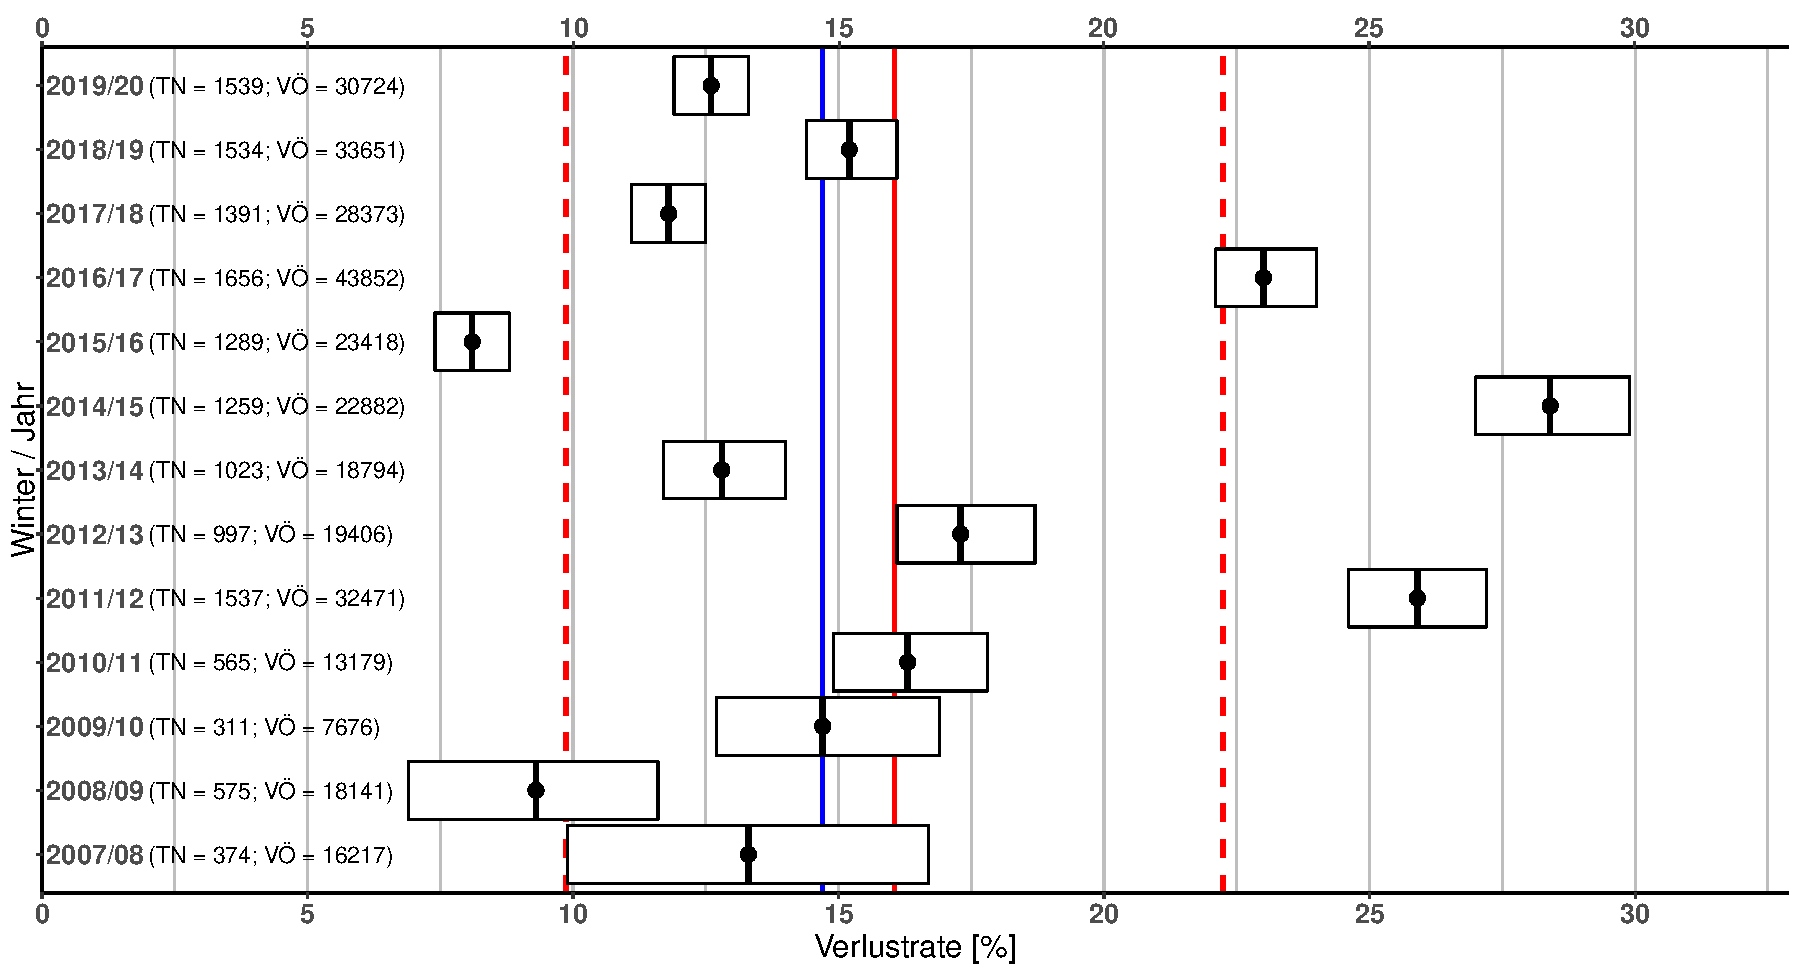
\includegraphics[keepaspectratio,width=1\textwidth]{project-U-wintersterblichkeit/figures/plot_years_losses}
  \caption{Höhe der Winterverluste in Österreich von 2007/08 bis 2019/20 in Prozent ($\pm$95\%CI). Rote Linie kennzeichnet den laufenden Mittelwert inklusive aktueller Umfrage; Rot strichlierte Linien Kennzeichnen die Standardabweichung vom Mittelwert. Blaue Linie kennzeichnet den Median Wert. TN = TeilnehmerInnen, VÖ = Gesamtsumme der eingewinterten Völker}
  \label{fig:u:years:losses}
\end{figure}
\newpage
\subsubsubsection{Populationsdynamik in Österreich}

Die Berechnungen zur Populationsdynamik basieren auf den Angaben jener Imkereien, die auch die Anzahl ihrer Völker im Frühjahr des Einwinterungsjahres bekannt gegeben haben (Subpopulation). Mit Hilfe dieser Information konnte die Netto-Änderung der Population bis zum Herbst desselben Jahres (Einwinterungsvölker) berechnet werden. Die Zahl an Bienenvölkern im Frühjahr des Auswinterungsjahres konnte aus der Differenz zwischen eingewinterten und der im Winter verlorenen Völker berechnet werden. Dies berücksichtigt aber nicht etwaige im Winter zugekaufte oder verkaufte Völker, sowie die Netto-Änderung über den Sommer. Die Informationen zur Anzahl der Völker im Frühjahr, eingewinterten Völkern und zum Völkerverlust über den Winter des jeweiligen Jahres ermöglichen eine grafische Darstellung der Populationsdynamik österreichischer Bienenvölker vom Frühjahr 2013 bis zum Frühjahr 2020 (\cref{fig:u:population}).
\newline
Ausgehend von der Völkeranzahl im Frühjahr des Einwinterungsjahres stieg die Zahl an Bienenvölkern durch Vermehrung und Zukäufe jeweils bis zum Herbst an (\cref{tab:u:population}, „Vermehrung über den Sommer [\%]``). Die prozentuelle Änderung der Anzahl der Bienenvölker vom Frühjahr des Auswinterungsjahres zum Frühjahr des Einwinterungsjahres ist in \cref{tab:u:population} („Vergleich Frühjahr-Frühjahr [\%]``) zu finden. Allgemein zeigt sich, dass die Vermehrung im Sommer manchmal eine konstante, manchmal sogar eine wachsende Bienenpopulation ermöglicht (\cref{fig:u:population}). Welche Netto-Zuwachsrate erforderlich wäre, um nach dem Winter wieder auf den Stand der Bienenpopulation im Herbst des Einwinterungsjahres zu kommen, ist unter „Ausgleich Verluste [\%]`` ersichtlich. 
\newline
Die tatsächliche Netto-Vermehrung über den Sommer liegt für das Untersuchungsjahr 2019/20 um 5,8\% über der Schätzung des letzten Jahres, in der berechnet worden war, welche Netto-Zuwachsrate erforderlich gewesen wäre, um eine konstante Population zu ermöglichen.

\begin{table}[H]
    \caption{Populationsdynamik der Subpopulation (Imkereien mit vollständigen Angaben) untersuchter österreichischer Bienenvölker vom Frühjahr 2013 bis zum Frühjahr 2020.}
    \label{tab:u:population}
    \scriptsize
    \begin{tabular}{|c|*{8}{r|}}
        \hline
        & & & 
        \multicolumn{3}{c|}{Anzahl Bienenvölker} & & 
        \multirow{2}{*}{\shortstack{Vergleich \\ Frühjahr-\\Frühjahr[\%]}} & 
        \\
        \cline{4-6}
        Jahr & 
        \makecell{Imkereien \\ [\textit{n}]} & 
        \makecell{Verlust- \\ rate [\%]$^1$} & 
        \makecell{Frühjahr [\#]$^2$} & 
        \makecell{Eingewintert \\ Herbst [\#]} & 
        \makecell{Ausgewintert \\ Frühjahr [\#]} & 
        \makecell{Vermehrung \\ Sommer [\%]} & 
        & 
        \makecell{Ausgleich \\ Verluste [\%]$^3$} 
        \\
        \hline
        2013/14 &   973 & 12,9 & 14.319 & 17.816 & 15.518 & 24,4 &   8,4 & 14,8 \\
        2014/15 & 1.188 & 28,6 & 17.355 & 21.616 & 15.437 & 24,6 & -11,1 & 40,0 \\
        2015/16 & 1.195 &  7,9 & 15.102 & 21.800 & 20.070 & 44,4 &  32,9 &  8,6 \\
        2016/17 & 1.537 & 22,5 & 27.695 & 40.141 & 31.108 & 44,9 &  12,3 & 29,0 \\
        2017/18 & 1.285 & 11,6 & 18.983 & 25.670 & 22.695 & 35,2 &  19,6 & 13,1 \\
        2018/19 & 1.465 & 15,3 & 24.747 & 31.036 & 26.277 & 25,4 &   6,2 & 18,1 \\
        2019/20 & 1.478 & 12,5 & 23.802 & 29.484 & 25.802 & 23.9 &   8,4 & 14,3 \\
        \hline
    \end{tabular}
    \scriptsize
    $^1$ Verlustrate der teilnehmende Imkereien mit vollständigen Angaben zur Anzahl der Völker im Frühjahr des Einwinterungsjahres.
    \newline
    $^2$ Völker im Frühjahr des Einwinterungsjahres.
    \newline
    $^3$ Erforderliche Netto-Zuwachsrate, um nach dem Winter wieder auf den Stand der Bienenpopulation im Herbst des Einwinterungsjahres zu kommen.
\end{table}



\myfig{project-U-wintersterblichkeit/figures/plot_population} % Pfad
  {width=0.8\textwidth} % Größe Relativ zu Text Breite
  {Veranschaulichte Populationsdynamik von Bienenvölkern der TeilnehmerInnen in Österreich vom Frühjahr 2013 bis zum Frühjahr 2020 basierend auf Winterverlusten und Vermehrung über den Sommer aus \cref{tab:u:population}. Diese theoretische Entwicklung der Völkeranzahl basiert auf einer Ausgangszahl von 100 Völkern. Rote Punkte sind die Anzahl an Bienenvölkern im Frühjahr des angegeben Jahres und blaue Punkte sind die Anzahl der Bienenvölker beim Einwintern.} % Text unterhalb der Grafik
  {Optionaler Kurz Titel} % Optional Kurz Überschrift
  {fig:u:population} % Label zum Verweisen im Text

\subsubsection{Bundesländer}

Zwischen den Bundesländern sind die Völkerverluste nicht gleichmäßig verteilt. Hier zeigen sich besonders für Wien signifikant höhere Verluste von \confi{20,1}{95}{16,0}{24,8} im Vergleich zu den anderen Bundesländern (ausgenommen Burgenland) und im Vergleich zum österreichischen Gesamtverlust (\cref{fig:u:states}). Die \cref{tab:u:states} zeigt die Anzahl der teilnehmenden Betriebe, die Anzahl der eingewinterten Völker, die Anzahl der verlorenen Völker, Winterverluste aufgrund von Königinnenproblemen und die Verlustrate in Summe und Prozent (inklusive 95\% Konfidenzintervall) für ganz Österreich und die einzelnen Bundesländer. Einen Überblick über die Winterverluste in ganz Österreich sowie in den Bundesländern für den gesamten Untersuchungszeitraum seit 2013/14, bietet die \cref{tab:u:states-year}. \cref{fig:u:states} zeigt eine grafische Darstellung der mittleren Verlustraten anhand einer Österreich-Karte.

\myfig{project-U-wintersterblichkeit/figures/plot_overview_states} % Pfad
  {width=0.9\textwidth} % Größe Relativ zu Text Breite
  {Höhe der Winterverluste 2019/20 für Österreich und die Bundesländer in Prozent ($\pm$95\%CI). Statistisch signifikante Ergebnisse sind mit einem Stern (*) gekennzeichnet.} % Text unterhalb der Grafik
  {} % Optional Kurz Überschrift
  {fig:u:states} % Label zum Verweisen im Text
  
 \myfig{project-U-wintersterblichkeit/figures/plot_map_loss_state} % Pfad
  {width=0.8\textwidth} % Größe Relativ zu Text Breite
  {Mittlere Verlustrate der Bundesländer, dargestellt anhand einer Österreich-Karte. Die Farbskala der Verlustraten beginnt bei 10\% für eine bessere Differenzierung der unterschiedlichen Verlustraten zwischen den Bundesländern.} % Text unterhalb der Grafik
  {Optionaler Kurz Titel} % Optional Kurz Überschrift
  {fig:u:states:map} % Label zum Verweisen im Text

\begin{table}[H]
    \caption{Teilnehmende Imkereibetriebe, eingewinterte Völker und Verlustraten von Bienenvölkern im Winter 2019/20 für Österreich und pro
    Bundesland. Völkerverluste durch „Elementarschaden (Flut, Vandalismus, etc.)`` (\sample{181}) sind nicht inkludiert.}
    \centering
    \scriptsize
    \label{tab:u:states}
    \begin{tabular}{l*{7}{r}}
        \toprule
        \makecell{Bundesland} &
        \makecell{Teilnehmende \\ Imkereien [n]} &
        \makecell{Völker \\ eingewintert[n]} &
        \makecell{Tote \\ Völker [n]} &
        \makecell{Verluste \\ (Königinnen-\\Probleme) [n]} &
        \makecell{Summe \\ Verlust [n]} &
        \makecell{Verlust \\ {[\%]}} &
        \makecell{CI {[\%]}} \\
        \midrule
        Österreich       & 1.539 & 30.724 & 2.539 & 1.334 & 3.873 & 12,6 & 11,9 - 13,3 \\
        Burgenland       &    33 &    521 &    31 &    23 &    54 & 10,4 &  6,3 - 16,6 \\
        Kärnten          &   151 &  3.743 &   338 &   140 &   478 & 12,8 & 10,8 - 15,0 \\
        Niederösterreich &   389 &  8.085 &   734 &   408 & 1.142 & 14,1 & 12,7 - 15,7 \\
        Oberösterreich   &   285 &  5.908 &   404 &   271 &   675 & 11,4 &  9,9 - 13,1 \\
        Salzburg         &    78 &  1.234 &    90 &    54 &   144 & 11,7 &  8,6 - 15,6 \\
        Steiermark       &   222 &  4.770 &   342 &   186 &   528 & 11,1 &  9,5 - 12,9 \\
        Tirol            &   153 &  3.699 &   308 &   149 &   457 & 12,4 & 10,4 - 14,6 \\
        Vorarlberg       &   136 &  1.568 &   106 &    49 &   155 &  9,9 &  7,4 - 13,1 \\
        Wien             &    92 &  1.196 &   186 &    54 &   240 & 20,1 & 16,0 - 24,8 \\
        \bottomrule
    \end{tabular}
\end{table}




\begin{table}[H]
    \caption{Vergleich der Winterverlustraten [\%] (\(\pm \)95\% Konfidenzintervall) von 2013/14 bis 2019/20 für Österreich sowie die einzelnen Bundesländer.}
    \centering
    \scriptsize
    %\setlength{\tabcolsep}{0.2em} % for the horizontal padding
    \label{tab:u:states-year}
    \begin{tabular}{|c|*{5}{rr|}}
        \hline    
        \multicolumn{1}{|c|}{Jahre} & 
        \multicolumn{2}{c|}{AUT}   & 
        \multicolumn{2}{c|}{Bgld.} & 
        \multicolumn{2}{c|}{Ktn.}  &  
        \multicolumn{2}{c|}{NÖ}    & 
        \multicolumn{2}{c|}{OÖ}    \\
        \hline
        
	    2013/14 & 12,8 & (11,7-14,0) & 32,9 & (15,1-57,5) &  9,9 &  (7,8-12,5) & 15,4 & (13,6-17,4) &  9,9 &  (7,6-12,8) \\
        2014/15 & 28,4 & (27,0-29,9) & 40,4 & (33,5-47,6) & 30,6 & (27,0-34,5) & 27,8 & (25,2-30,6) & 25,2 & (21,6-29,2) \\
        2015/16 &  8,1 &   (7,4-8,8) & 11,0 &  (6,7-17,6) &  6,6 &   (5,4-7,9) & 11,5 &  (9,8-13,5) &  6,8 &   (5,5-8,4) \\
        2016/17 & 23,0 & (22,1-24,0) & 20,2 & (15,2-26,4) & 21,9 & (18,6-25,6) & 24,2 & (22,8-25,7) & 18,9 & (16,7-21,4) \\
        2017/18 & 11,8 & (11,1-12,5) &  7,9 &  (4,8-12,7) & 14,5 & (10,5-15,7) & 12,3 & (12,5-15,2) &  9,9 & (10,1-13,1) \\
        2018/19 & 15,2 & (14,4-16,1) &  9,9 &  (6,9-13,9) & 11,5 &  (9,4-14,1) & 17,0 & (15,3-18,7) & 17,5 & (15,5-19,8) \\
        2019/20 & 12,6 & (11,9-13,3) & 10,4 &  (6,3-16,6) & 12,8 & (10,8-15,0) & 14,1 & (12,7-15,7) & 11,4 &  (9,9-13,1) \\

        \hline    
        \multicolumn{1}{|c|}{Jahre} & 
        \multicolumn{2}{c|}{Sbg.}  & 
        \multicolumn{2}{c|}{Stmk.} &
        \multicolumn{2}{c|}{T}     &
        \multicolumn{2}{c|}{Vbg.}  &
        \multicolumn{2}{c|}{W}     \\
        \hline

        2013/14 & 18,6 & (13,5-25,1) &  8,5 &  (6,7-10,7) & 12,9 &  (9,0-18,1) & 18,1 & (12,1-26,2) & 19,2 & (12,7-27,9) \\
        2014/15 & 33,6 & (27,3-40,5) & 22,5 & (19,4-25,8) & 26,7 & (21,6-32,4) & 28,0 & (22,3-34,4) & 52,6 & (44,9-60,2) \\
        2015/16 &  6,1 &   (4,1-9,1) &  8,7 &  (7,0-10,6) &  5,1 &   (3,7-6,9) &  5,8 &   (3,7-9,1) & 11,5 &  (7,2-17,8) \\
        2016/17 & 16,8 & (12,3-22,6) & 19,3 & (17,0-21,9) & 25,1 & (20,6-30,3) & 33,8 & (29,5-38,3) & 24,8 & (20,2-30,0) \\
        2017/18 & 10,8 &  (9,1-17,5) &  8,2 &  (7,3-10,3) & 12,0 &  (9,0-14,6) & 10,1 &  (8,1-12,5) & 14,4 &  (9,3-16,0) \\
        2018/19 & 16,2 & (11,7-22,1) & 13,0 & (11,0-15,3) & 11,4 &  (9,3-14,0) & 17,7 & (15,0-20,8) & 19,6 & (14,9-25,3) \\
        2019/20 & 11,7 &  (8,6-15,6) & 11,1 &  (9,5-12,9) & 12,4 & (10,4-14,6) &  9,9 &  (7,4-13,1) & 20,1 & (16,0-24,8) \\

        \hline
    \end{tabular}

\end{table}


\newpage 

\subsubsection{Ausgewählte Bezirke}

Die Verlustraten, Anzahl der teilnehmenden Imkereien und Anzahl der eingewinterten Völker auf Bezirksebene sind im Anhang in den Tabellen \crefrange{tab:u:district-burgenland}{tab:u:district-wien} aufgelistet. Die Ergebnisse der vorangegangenen Untersuchungsjahre sind in den Tabellen zum Vergleich ebenfalls dargestellt. \cref{fig:u:map:loss:district} zeigt die mittleren Verlustraten der Bezirke als Karte. Aus Gründen des Datenschutzes und der Repräsentativität werden nur jene Bezirke aufgelistet, bei denen mindestens Daten von fünf Imkereien zur Verfügung stehen. Hier sei noch einmal angemerkt, dass die Berechnung der Verlustraten in unserer Analyse auf den jeweiligen Gesamtzahlen basiert, dh. Summe der eingewinterten Völker und die Summe der verlorenen Völker, und nicht auf Betriebsebene durchgeführt wird.

\myfig{project-U-wintersterblichkeit/figures/plot_map_loss_district} % Pfad
  {width=0.8\textwidth} % Größe Relativ zu Text Breite
  {Mittlere Verlustrate der einzelnen Bezirke. Weiße Bezirke < 5 Antworten.} % Text unterhalb der Grafik
  {Optionaler Kurz Titel} % Optional Kurz Überschrift
  {fig:u:map:loss:district} % Label zum Verweisen im Text

\subsection{Symptome}

Für eine umfassende Analyse der Winterverluste ist es wichtig, die Symptome, welche mit den Völkerverlusten einhergehen, zu kennen. Imkereien mit Winterverlusten wurden daher gebeten, die an ihren Völkern beobachteten Symptome zu nennen. Folgende einfach und ohne weitere Hilfsmittel zu beurteilende Symptome standen zur Auswahl: a) hatten viele tote Bienen im oder vor dem Volk, b) hatten keine oder nur wenige tote Bienen im oder vor dem Volk, c) hatten tote Bienen in Zellen, und kein Futter im Stock (verhungert), d) hatten tote Bienen in Zellen, aber genug Futter im Stock (Futter nicht erreicht), e) hatten keine der oben genannten oder unbekannte Symptome. \cref{fig:u:loss:symptome} zeigt die Häufigkeiten der die Winterverluste 2019/20 begleitenden Symptome. 
\\
Zur Berechnung der relativen Häufigkeit wurden nur jene ImkerInnen genommen, welche Verluste und Symptome gemeldet haben. Mehrfachnennungen von mehreren Symptomen waren möglich, wobei einzelne Symptomtypen aber maximal gleich hoch sein konnten wie die gemeldeten Verluste. Ingesamt haben 710 TeilnehmerInnen 2.503 Symptomnennungen zu ihren 3.366 verloren Völkern gemacht. Das häufigste Symptom war \enquote{b) hatten keine oder nur wenige tote Bienen im oder vor dem Volk} mit 39,9\%, gefolgt von \enquote{a) hatten viele tote Bienen im oder vor dem Volk} mit 14,1\% und \enquote{d) hatten tote Bienen in Zellen, aber genug Futter im Stock (Futter nicht erreicht)} mit 10.9\%. Ein klassisches Verhungern \enquote{c) hatten tote Bienen in Zellen, und kein Futter im Stock (verhungert)} wurde mit einer Häufigkeit von 5,6\% gemeldet und am wenigsten häufig war \enquote{e) hatten keine der oben genannten oder unbekannte Symptome} mit 3,9\% (\cref{fig:u:loss:symptome}).

\begin{figure}[H]
 \centering
 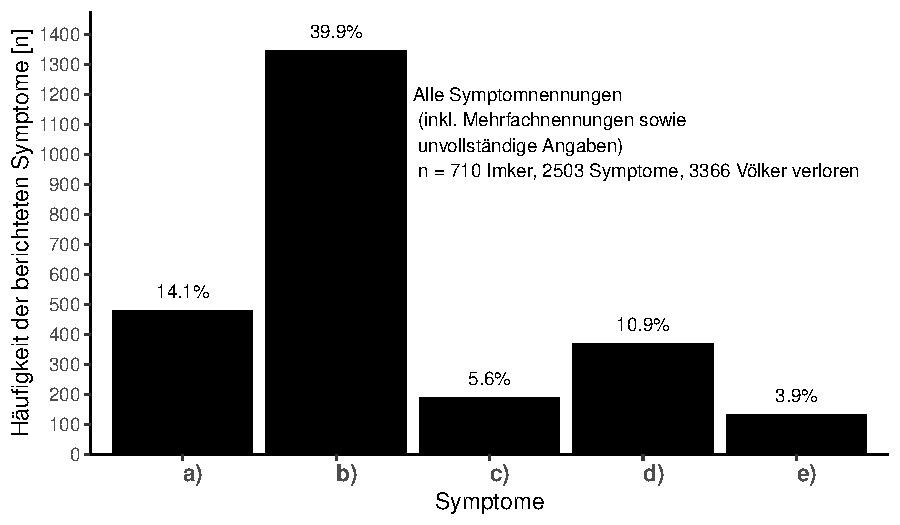
\includegraphics[keepaspectratio,width=0.8\textwidth]{project-U-wintersterblichkeit/figures/plot_symptome}
 \caption{Häufigkeit der von ImkerInnen berichteten Symptome inklusive Mehrfachnennungen und unvollständigen Angaben a) bis e) in Prozent für 2019/20: a) Viele tote Bienen im oder vor dem Volk, b) keine oder nur wenige tote Bienen im oder vor dem Volk, c) tote Bienen in Zellen, kein Futter im Stock, d) tote Bienen in Zellen, aber genug Futter im Stock, e) keines der oben genannten oder unbekannte Symptome.}
 \label{fig:u:loss:symptome}
\end{figure}

\newpage 

\subsection{Verteilung der Völkerverluste}

Für die Berechnung der Verteilung der Völkerverluste wird für jeden einzelnen Imkereibetrieb die Höhe des Gesamtverlustes (d.h. die Summe der toten oder verlorenen Völker und der von Königinnenproblemen betroffenen Völker) der insgesamt eingewinterten Völker in Prozent berechnet. Insgesamt haben 35,6\% unserer TeilnehmerInnen keine Verluste erlitten. Zwischen >0-20\% haben 38,5\% der ImkerInnen Verluste gemeldet (\cref{fig:u:loss:distribution}). Verluste über 20\% haben 25,9\% der TeilnehmerInnen angegeben.

\begin{figure}[H]
  \centering
  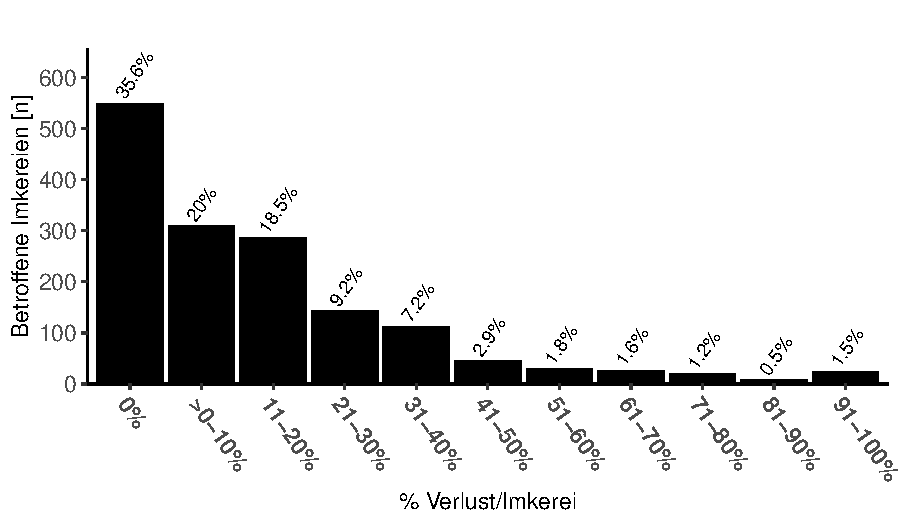
\includegraphics[keepaspectratio,width=0.8\textwidth]{project-U-wintersterblichkeit/figures/plot_overview_loss_dist}
  \caption{Verteilung der Verluste in Prozent pro teilnehmender Imkerei in 10\%-Verlustgruppen, extra angeführt sind TeilnehmerInnen ohne Verluste in der Gruppe \enquote{0\%}.}
  \label{fig:u:loss:distribution}
\end{figure}

\subsection{Risikoanalyse}

In der Risikoanalyse werden die Winterverlustraten verschiedener Gruppen von Betriebsweisen miteinander verglichen. Besteht beispielsweise zwischen zwei Gruppen von Betriebsweisen ein signifikanter Unterschied, kann man daraus Schlussfolgerungen über die Bedeutung dieses Risikofaktors für Winterverluste von Bienenvölkern ziehen. Überlappen die Konfidenzintervalle der Verlustraten von zwei oder mehreren Gruppen nicht, kann die untersuchte Betriebsweise, oder andere damit verknüpfte aber nicht erhobene Faktoren, als signifikanter Einflussfaktor auf die Höhe der Winterverluste betrachtet werden. In weiterer Folge werden die folgenden Faktoren dargestellt:
\ref{ss:seehoehe:U} \nameref{ss:seehoehe:U},
\ref{ss:betriebsgroesse:U} \nameref{ss:betriebsgroesse:U},
\ref{ss:betriebsweise:U} \nameref{ss:betriebsweise:U},
\ref{ss:stand_wander:U} \nameref{ss:stand_wander:U},
\ref{ss:vereinigung:U} \nameref{ss:vereinigung:U},
\ref{ss:wabenhygiene:U} \nameref{ss:wabenhygiene:U},
\ref{ss:trachtangebot:U} \nameref{ss:trachtangebot:U},
\ref{ss:baekempfung_varroa:U} \nameref{ss:baekempfung_varroa:U},
\ref{ss:koeniginnen_verluste:U} \nameref{ss:koeniginnen_verluste:U},
\ref{ss:koeniginnen_probleme:U} \nameref{ss:koeniginnen_probleme:U},
\ref{ss:junge_koeniginnen:U} \nameref{ss:junge_koeniginnen:U},
\ref{ss:verkeuppelte_fluegel:U} \nameref{ss:verkeuppelte_fluegel:U}.


\subsubsection{Seehöhe}
\label{ss:seehoehe:U}

Um den Einfluss der Seehöhe auf die Wintersterblichkeit von Bienenvölkern zu untersuchen, wurden die Winterstandorte bezüglich ihrer Seehöhe in fünf Klassen eingeteilt: 0-200~m, 201-400~m, 401-600~m, 601-800~m, >800~m. Um die Genauigkeit der Auswertung zu erhöhen wurden TeilnehmerInnen die \enquote{Nein} oder \enquote{Unsicher} bei der Fragestellung \enquote{Alle Bienenvölker innerhalb eines \SI{15}{\kilo\meter} Radius} angaben sowie ihre Bienenstände in \enquote{mehr als einem Bezirk} verteilt haben in dieser Risikoanalyse nicht beachtet.
\newline
Im Untersuchungsjahr 2019/20 konnte eine signifikant niedrigere Verlustrate bei der Gruppe „>800 m`` mit \confi{11,6}{95}{10,0}{13,4} und der Gruppe „401-600 m`` mit \confi{11,9}{95}{10,6}{13,3} im Vergleich zu der Gruppe „201-400 m`` mit \confi{15,4}{95}{13,8}{17,3}
festgestellt werden.
\newline
Die Verlustraten der zwei restlichen Gruppen verteilen sich wie folgt: Gruppe „0-200 m`` mit \confi{15,3}{95}{12,0}{19,4} und Gruppe „601-800 m`` mit \confi{13,0}{95}{11,0}{15,3}.

\begin{figure}[H]
  \centering
  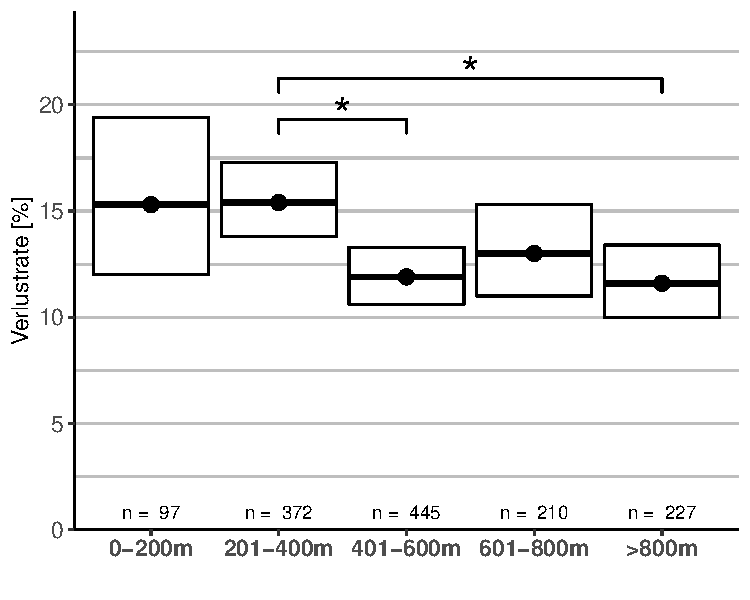
\includegraphics[keepaspectratio,width=0.6\textwidth]{project-U-wintersterblichkeit/figures/plot_elevation}
  \caption{Höhe der Winterverluste 2019/20 in Prozent ($\pm$95\%CI) in Abhängigkeit von der Seehöhe der Winterstandorte. Nicht ausgewertet sind TeilnehmerInnen die \enquote{Nein} oder \enquote{Unsicher} bei Fragestellung \enquote{Alle Bienenvölker innerhalb eines \SI{15}{\kilo\meter} Radius} angaben, sowie ihre Bienenvölker in \enquote{mehr als einem Bezirk} aufgestellt haben. Statistisch signifikante Ergebnisse sind mit einem Stern (*) gekennzeichnet.}
  \label{fig:u:elevation}
\end{figure}

\subsubsection{Betriebsgröße}
\label{ss:betriebsgroesse:U}

Die Analyse der Erhebung 2019/20 hat gezeigt, dass die Betriebsgröße von Imkereien, wie auch in vergangenen Jahren, einen Risikofaktor für Winterverluste darstellt.
\newline
Es zeigt sich eine signifikant niedrigere Verlustrate für ImkerInnen mit mehr als 50 Völkern (\confi{10,2}{95}{9,2}{11,2}) im Vergleich zu der Gruppe mit 1-50 Völkern mit \confi{14,1}{95}{13,2}{15,0} (\cref{fig:u:factor:operationsize}-A). Wurde diese Aufgliederung zur genaueren Betrachtung in drei Gruppen (Betriebe mit 1 bis 20 Völkern, solche mit 21-50 Völkern und Betriebe mit mehr als 50 Völkern) anstatt zwei unterteilt, zeigten sich 2019/20 signifikant höhere Verluste bei der Gruppe „1-20`` mit \confi{15,1}{95}{13,9}{16,4} und der Gruppe „21-50`` mit \confi{12,9}{95}{11,7}{14,3} im Vergleich zur Gruppe mit über 50 Völkern (\cref{fig:u:factor:operationsize}-B).

\myfig{project-U-wintersterblichkeit/figures/plot_factor_operationsize_combined} % Pfad
  {width=1\textwidth} % Größe Relativ zu Text Breite
  {Höhe der Winterverluste 2019/20 in Prozent ($\pm$95\%CI) in Abhängigkeit von der Betriebsgröße. (A) Einteilung in 1-50 und >50 Völker. (B) Einteilung in 1-20, 21-50 und >50 Völker. Statistisch signifikante Ergebnisse sind mit einem Stern (*) gekennzeichnet.} % Text unterhalb der Grafik
  {Optionaler Kurz Titel} % Optional Kurz Überschrift
  {fig:u:factor:operationsize} % Label zum Verweisen im Text

\subsubsection{Betriebsweise}
\label{ss:betriebsweise:U}

Seit 2016/17 werden die ImkerInnen, auch auf eigenen Wunsch, zu weiteren Details ihrer Betriebsweise befragt. Dabei konnten Angaben zu den Beuten gemacht und festgehalten werden, ob der Betrieb eine zertifizierte Bio-Imkerei ist, eine Wanderimkerei betreibt, Bienen auf Varroa-Toleranz züchtet, Fremdwachs zukauft oder neu seit 2019/20 ob schwache (weiselrichtige) Völker vor dem Winter zusammegelegt wurden.
\newline
Über die Hälfte der TeilnehmerInnen haben angegeben einen offenen Gitterboden in ihren Beuten im Winter zu verwenden und circa 50\% haben Wachs von außerhalb des Betriebes zugekauft. Wie auch in der vorjährigen Befragung gab nur ein kleiner Anteil an Betrieben (7,8\%) an \enquote{Naturwabenbau ohne Mittelwand} zu verwenden. Zertifizierte Bio-Imkereien waren mit 183 Betrieben in der Befragung vertreten. Einen Überblick über die Häufigkeit der verschiedenen Betriebsweisen (Angaben: „Ja``, „Nein``, „Unsicher``, „keine Angaben``) bietet die \cref{fig:u:operational:hist}. 
\newline
\cref{fig:u:operational:loss} zeigt den Einfluss der verschiedenen Betriebsweisen auf die Winterverlustraten. In diesem Untersuchungsjahr konnte eine signifikant niedrigere Verlustrate bei TeilnehmerInnen mit Völkern aus \enquote{Zucht aus Varroa-Toleranz} mit \confi{10,3}{95}{8,5}{12,4} im Gegensatz zur Gruppe \enquote{Unsicher} mit \confi{16,7}{95}{12,7}{21,5} gezeigt werden. Kein statistischer Unterschied war zur Gruppe \enquote{Nein} mit einer Verlustrate von \confi{12,7}{95}{12,0}{13,6} (\cref{fig:u:operational:loss}-C) zu erkennen. TeilnehmerInnen die Fremdwachs eingesetzt haben zeigten eine signifikant höhere Verlustrate mit \confi{14,8}{95}{13,4}{16,3} im Gegensatz zu Imkereibetrieben mit eigenem Wachskreislauf (\confi{11,7}{95}{10,9}{12,6}) (\cref{fig:u:operational:loss}-G). Es konnte auch ein signifikanter Unterschied festgestellt werden bei der Frage ob \enquote{Kleine Brutzellen (5,1 mm oder weniger)} verwendet wurden. Hier zeigt sich eine signifikant niedrigere Verlustrate für die Gruppe \enquote{Ja} mit \confi{6,8}{95}{4,9}{9,4} im Gegensatz zu den anderen zwei Gruppen (Nein - \confi{12,6}{95}{11,8}{13,4}, Unsicher - \confi{16,6}{95}{12,7}{21,4}) (\cref{fig:u:operational:loss}-I).
\newline
Kein statistisch signifikanter Unterschied konnte festgestellt werden zwischen Bio-Imkereien \confi{11,3}{95}{10,1}{12,6} und nicht zertifizierten Bio-ImkerInnen \confi{12,5}{95}{11,7}{13,4}. Auch kein Unterschied konnte bei der Frage \enquote{Naturwabenbau} beobachtet werden (Ja - \confi{12,6}{95}{10,3}{15,3}, Nein - \confi{12,6}{95}{11,8}{13,4}, Unsicher - \confi{10,6}{95}{7,3}{15,1}). Die Fragen zur Bauart des Bienenstockes hatten in unserer Untersuchung auch keinen Einfluss: \enquote{Kunststoff-Beuten} (Ja - \confi{12,2}{95}{10,2}{14,5}, Nein - \confi{12,5}{95}{11,7}{13,3}); \enquote{Isolierte Beuten im Winter} (Ja - \confi{13,6}{95}{12,0}{15,4}, Nein - \confi{12,6}{95}{11,8}{13,5}, Unsicher - \confi{15,2}{95}{10,2}{22,0}) und \enquote{Offener Gitterboden im Winter} (Ja - \confi{12,9}{95}{12,0}{14,0}, Nein - \confi{12,0}{95}{11,0}{13,1}) (\cref{fig:u:operational:loss}-A,D,E,F,H).

\begin{figure}[H]
  \centering
  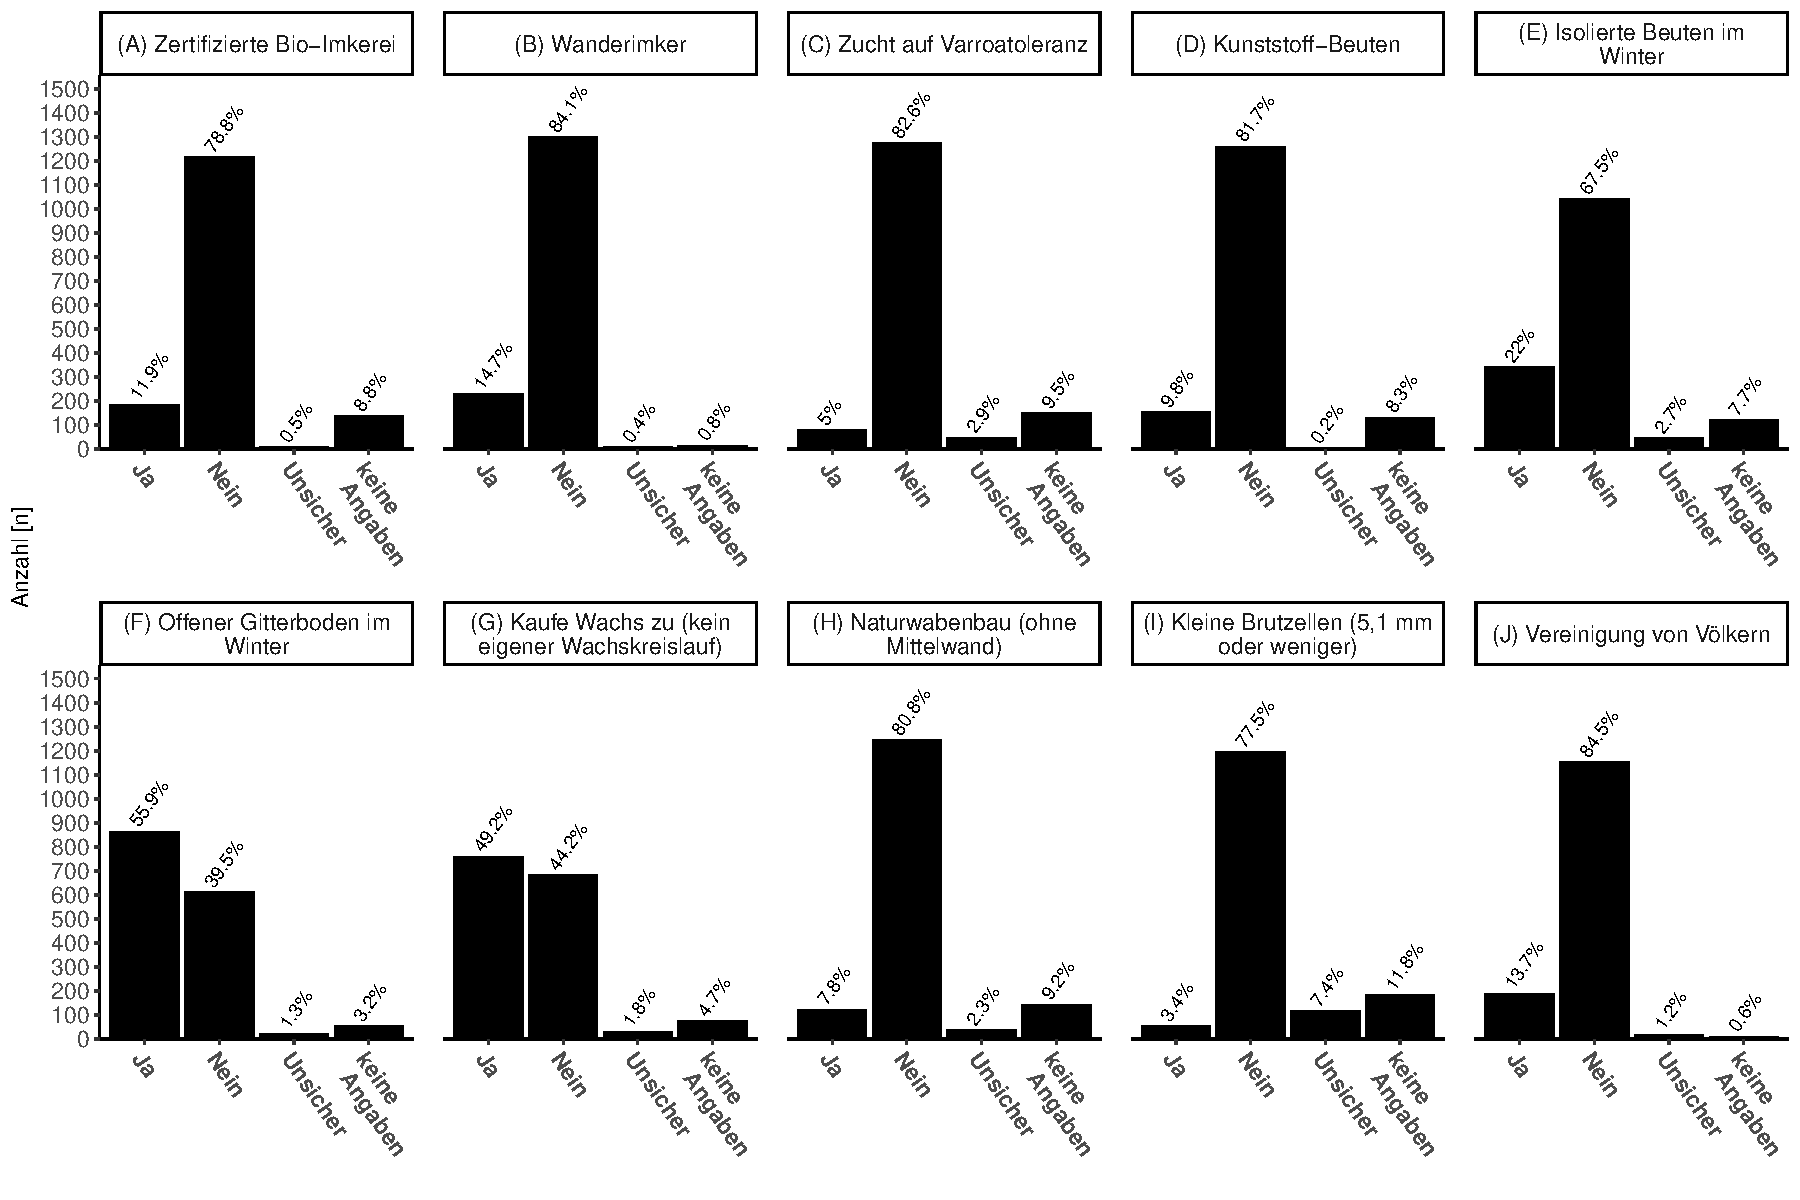
\includegraphics[keepaspectratio,width=1\textwidth]{project-U-wintersterblichkeit/figures/plot_operational_hist}
  \caption{Häufigkeit der Betriebsweisen 2019/20 in unserer Umfrage inklusive Angabe in Prozent.}
  \label{fig:u:operational:hist}
\end{figure}

\subsubsubsection{Stand- versus Wanderimkereien}
\label{ss:stand_wander:U}

Für den Winter 2019/20 wurde untersucht, ob sich Wanderimkerei auf die Wintersterblichkeit auswirkt. Die an unserer Studie teilnehmenden ImkerInnen wurden gefragt, ob sie ihre Bienen zu Trachtquellen oder Bestäubungseinsätzen transportieren (Verbringungen im Zuge der Zucht oder Ablegerbildung sind damit exkludiert).
\newline
Es konnte eine signifikant geringere Verlustrate bei Wanderimkereien (\confi{10,5}{95}{9,4}{11,7}) im Vergleich zu Standimkereien mit \confi{13,8}{95}{12,9}{14,7} festgestellt werden (\cref{fig:u:operational:loss}-B). 

\subsubsubsection{Vereinigung von Völkern}
\label{ss:vereinigung:U}

Neu in der Umfrage 2019/20 ist die Frage ob bereits vor dem Winter schwache (aber weiselrichtige) Völker vereinigt wurden. Insgesamt gaben 13,7\% der TeilnehmerInnen an Völker bereits vor dem Winter zu vereinigen. Zur Winterverlustrate zeigt sich hier kein statistischer Unterschied zwischen den Gruppen (Ja - \confi{12,7}{95}{11,1}{14,4}, Nein - \confi{12,1}{95}{11,3}{13,0}) (\cref{fig:u:operational:loss}-J).

\begin{figure}[H]
  \centering
  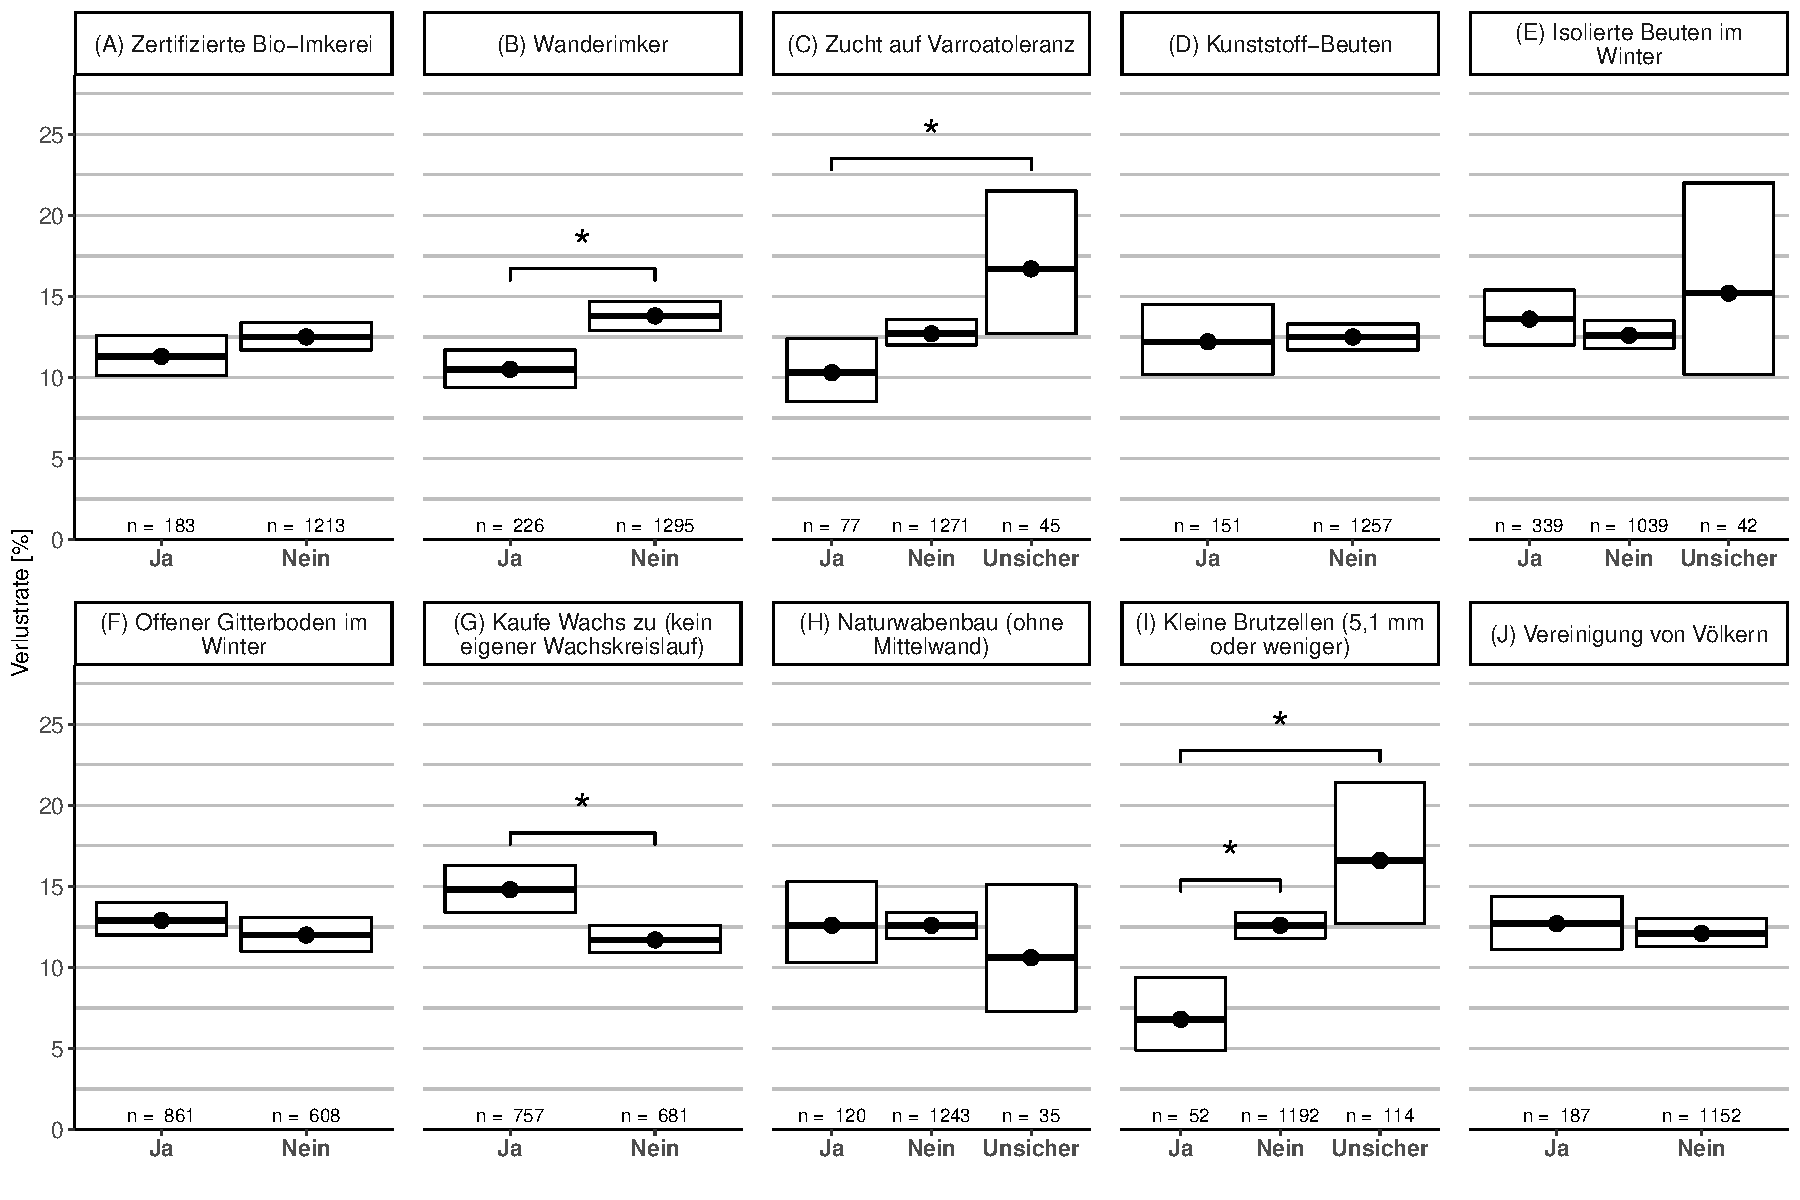
\includegraphics[keepaspectratio,width=1\textwidth]{project-U-wintersterblichkeit/figures/plot_operational_loss}
  \caption{Höhe der Winterverluste 2019/20 in Prozent ($\pm$95\%CI) in Abhängigkeit von der Betriebsweise der TeilnehmerInnen. Die Gruppe mit der Angabe\enquote{Unsicher} wurde nicht ausgewertet wenn \textit{n}<30. Statistisch signifikante Ergebnisse sind mit einem Stern (*) gekennzeichnet.}
  \label{fig:u:operational:loss}
\end{figure}
\newpage
\subsubsection{Wabenhygiene}
\label{ss:wabenhygiene:U}

Wabenhygiene in Form von Erneuerung alter Brutwaben kann einen positiven Einfluss auf die Gesundheit der Bienen haben und möglicherweise auch das Überleben der Bienen im Winter beeinflussen. Die ImkerInnen wurden gefragt, welchen Anteil ihrer Brutwaben (in Prozentklassen) sie erneuert haben. In diesem Jahr konnte kein statistischer Unterschied der Verlustraten zwischen den Gruppen festgestellt werden: Keine Brutwaben erneuert - \confi{14,8}{95}{7,1}{28,4}; Gruppe 1-30\% - \confi{14,2}{95}{12,5}{16,0}; Gruppe 31-50\% - \confi{11,4}{95}{10,4}{12,5} und die Gruppe mit der meisten Erneuerung 51-100\% mit \confi{12,3}{95}{11,2}{13,5}. Die Gruppe der TeilnehmerInnen die zu dieser Frage \enquote{keine Angaben} gemacht hatten zeigt eine Verlustrate von \confi{16,5}{95}{11,4}{23,3} (\cref{fig:u:factor:frames}).

\myfig{project-U-wintersterblichkeit/figures/plot_factor_frames} % Pfad
{width=0.6\textwidth} % Größe Relativ zu Text Breite
{Höhe der Winterverluste von 2019/20 in Abhängigkeit vom Anteil der im Einwinterungsjahr erneuerten Brutwaben in Prozentklassen ($\pm $95\%CI).} % Text unterhalb der Grafik
{Optionaler Kurz Titel} % Optional Kurz Überschrift
{fig:u:factor:frames} % Label zum Verweisen im Text

\subsubsection{Trachtangebot}
\label{ss:trachtangebot:U}

Die teilnehmenden ImkerInnen wurden nach spezifischen Trachtquellen gefragt, die von ihren Bienen beflogen wurden, um mögliche Risikotrachtquellen zu bestimmen. Zur Auswahl standen 2019/20: Raps (\textit{Brassica napus}), Mais (\textit{Zea mays}), Sonnenblume (\textit{Helianthus annuus}), spätblühende Zwischenfrüchte, Waldtracht sowie Waldtracht mit Melezitose.
\newline
TeilnehmerInnen die eine Rapstracht hatten zeigten statistisch signifikant höhere Verlustraten (Ja - \confi{13,8}{95}{12,2}{15,5}; Nein - \confi{11,5}{95}{10,7}{12,4}; $\chi^{2}$=20,9, \textit{p}<0,05) (\cref{fig:u:factor:yield}-A). Auch ImkerInnen deren Bienen Mais beflogen zeigten signifikant höhere Verluste (Ja - \confi{17,7}{95}{14,8}{21,0}; Nein - \confi{11,6}{95}{10,8}{12,5}) (\cref{fig:u:factor:yield}-B).
\newline
Ein positiver Effekt konnte bei der Waldtracht festgestellt werden, hier zeigte sich eine signifikant geringere Verlusterate wenn eine Tracht vorhanden war (Ja - \confi{11,4}{95}{10,5}{12,3}; Nein - \confi{14,4}{95}{12,8}{16,2}) (\cref{fig:u:factor:yield}-E).
\newline
Kein statistischer Unterschied konnte bei den anderen in der Umfrage angeführten Trachtquellen festgestellt werden: Sonnenblume (Ja - \confi{14,0}{95}{12,2}{16,0}; Nein - \confi{12,0}{95}{11,1}{12,9}); Spätblüher (Ja - \confi{12,6}{95}{11,6}{13,8}; Nein - \confi{12,6}{95}{11,2}{14,1}) und auch nicht bei Waldtracht mit Melezitose (Ja - \confi{11,6}{95}{10,7}{12,6}; Nein - \confi{13,5}{95}{12,3}{14,8}) (\cref{fig:u:factor:yield}-C,D,F).
\newline
Zur groben Feststellung der Trachtgebiete wurde anhand der Haupt-Überwinterungsstandorte (ohne WanderimkerInnen) eine Karte der betroffenen ImkerInnen aufgezeichnet, welche im Anhang angeführt ist, siehe \cref{fig:u:factor:yield_map}.

\myfig{project-U-wintersterblichkeit/figures/plot_factor_yield} % Pfad
{width=1\textwidth} % Größe Relativ zu Text Breite
{Höhe der Winterverluste von 2019/20 in Abhängigkeit vom Vorhandensein spezifischer Trachtpflanzen in Prozent ($\pm$95\%CI); n=~Anzahl der Betriebe inklusive Wanderimkereien. Statistisch signifikante Ergebnisse sind mit einem Stern (*) gekennzeichnet.} % Text unterhalb der Grafik
{Optionaler Kurz Titel} % Optional Kurz Überschrift
{fig:u:factor:yield} % Label zum Verweisen im Text

\newpage

\subsubsection{Bekämpfung der Varroamilbe}
\label{ss:baekempfung_varroa:U}

Ein wichtiger Teil der Untersuchung sind Erhebungen über die Behandlungsmethoden gegen die Varroamilbe und deren Auswirkung auf die Winterverluste. \cref{fig:u:behandlungsmethoden} zeigt die am Fragebogen zur Auswahl gestellten Behandlungsmethoden. Dabei wird aus Gründen der internationalen Vergleichbarkeit, der von COLOSS erarbeitete Katalog von möglichen Bekämpfungsmethoden verwendet. Nachfolgend wird zuerst die Häufigkeit der verwendeten Methoden dargestellt. Anschließend wurden die einzelnen Methoden im Hinblick auf ihren Einfluss auf die Winterverlustrate betrachtet. Für die detaillierte Risikoanalyse wurden nur jene Behandlungsmethoden berücksichtigt, von denen auch genügend Datensätze vorhanden waren, um eine valide Aussage treffen zu können. Bei der Befragung mittels dem verkürzten Zeitschriftfragebogen wurden keine Details zur Behandlung abgefragt.

\myfig{project-U-wintersterblichkeit/figures/img_behandlungen.png} % Pfad
{width=0.8\textwidth} % Größe Relativ zu Text Breite
{Im Fragebogen zur Auswahl stehende Behandlungsmethoden gegen die Varroamilbe.} % Text unterhalb der Grafik
{Optionaler Kurz Titel} % Optional Kurz Überschrift
{fig:u:behandlungsmethoden} % Label zum Verweisen im Text

91\% der Imkereien bestimmten in mindestens einem Monat des abgefragten Zeitraums den Varroabefall ihrer Völker (zum Beispiel natürlicher Milbenfall mit Stockwindel oder Diagnose mittels Staubzuckermethode) (\cref{tab:u:varroakontrolle}). 
\newline
\cref{tab:u:behandlungsmethoden} zeigt die durchgeführten Methoden der Varroabekämpfung von allen Imkereien, die uns Daten im Untersuchungszeitraum von 2019/20 zur Verfügung gestellt haben.

Eine der häufigsten Methoden zur Varroabekämpfung ist die Drohnenbrutentnahme, welche von 54,3\% der ImkerInnen in zumindest einem Monat durchgeführt wurde. Danach folgten, nach Häufigkeit der Anwendung, Bekämpfungsmaßnahmen mit organischen Säuren (Ameisensäure Kurzzeit oder Langzeit, unterschiedliche Anwendungsformen der Oxalsäure). Insgesamt 74,8\% der TeilnehmerInnen führte eine Ameisensäurebehandlung durch (Kurzzeit und/oder Langzeit, wobei Langzeitbehandlungen mit 49,1\% etwas häufiger angewandt werden). Von den unterschiedlichen Anwendungen der Oxalsäure, wird die Verdampfung von 51,8\% aller Imkereien angewandt, das Träufeln oder Sprühen von 35,9\% und das Träufeln von Oxalsäureprodukten mit weiteren Inhaltsstoffen (Hiveclean/Bienenwohl/Varromed) von 26,9\% der Imkereien. Die Kombinationsanwendung der beiden organischen Säuren (Ameisensäure kurz oder lang, sowie eine Restentmilbung mit Oxalsäure) wird von 69,3\% der österreichischen Imkereien angewandt. Thymol, egal ob in alleiniger Anwendung oder in Kombination mit anderen Methoden, wurde von 7,7\% der Imkereien als Methode zur Bekämpfung der Varroamilbe verwendet. Biotechnische Methoden abseits der Drohnenbrutentnahme oder Hyperthermie wurden von 25,7\% der Imkereien angewandt, dazu zählen etwa die Fangwabe, die Bannwabe oder die totale Brutentnahme. Hyperthermie (=Hitzebehandlung) oder Milchsäure wurden von 4,6\% beziehungsweise 3,5\% der Imkereien angewandt. Synthetische Akarizide zur Bekämpfung der Varroamilbe wurden nur in einem geringen Ausmaß genannt (2,5\%), wobei am häufigsten Amitraz (0,6\%) (Streifen oder Verdampfen) genannt wurde.

\begin{table}[H]
    \centering
    \caption{Anzahl (Prozent) der Imkereien, welche eine Kontrolle der Varroamilbe in zumindest einem Monat durchgeführt haben.}
    \label{tab:u:varroakontrolle}
    \begin{tabular}{l|*{2}{rr|}rr}
        %\hline
            \multicolumn{1}{c}{} & 
            \multicolumn{2}{c|}{Ja} & 
            \multicolumn{2}{c|}{Nein} &
            \multicolumn{2}{c}{keine Angaben} \\ 
        \cline{2-7}
            \multicolumn{1}{c}{} & 
            \makecell{\textit{n}} & \makecell{{\%}} & \makecell{\textit{n}} & \makecell{{\%}} & \makecell{\textit{n}} & \makecell{{\%}} \\
        \hline
        \makecell[l]{Bestimmung Varroabefall \\ (Milbenfall o. ä. Methode)} 
        & 1309 & 91,0\% & 76 & 5,3\% & 54 & 3,8\% \\
        \hline
    \end{tabular}
\end{table}



\begin{table}[H]
    \centering
    \caption{Anzahl (Prozent) der Imkereien, welche die genannte Methode zur Bekämpfung der Varroamilbe in zumindest einem Monat angewendet haben.}
    \label{tab:u:behandlungsmethoden}
    \begin{tabular}{l|*{1}{rr|}rr}
        \toprule            \multirow{2}{*}{\makecell{Behandlungsmethode}} & 
            \multicolumn{2}{c|}{Ja} & 
            \multicolumn{2}{c}{Nein} \\ 
        \cline{2-5}
            & \makecell{\textit{n}} & \makecell{{\%}} & \makecell{\textit{n}} & \makecell{{\%}} \\
        \midrule
        Drohnenbrutentnahme 
        & 778 & 54,3 & 655 & 45,7 \\

        Hyperthermie
        & 66 & 4,6 & 1367 & 95,4 \\

        Andere biotechnische Methode$^1$
        & 368 & 25,7 & 1065 & 74,3 \\

        Ameisensäure KB$^2$ (inkl. MAQS)
        & 538 & 37,5 & 895 & 62,5 \\

        Ameisensäure LB$^2$
        & 703 & 49,1 & 730 & 50,9 \\

        Milchsäure 
        & 50 & 3,5 & 1383 & 96,5 \\

        Oxalsäure Träufeln (oder Sprühen) 
        & 514 & 35,9 & 919 & 64,1 \\

        Oxalsäure Verdampfen
        & 742 & 51,8 & 691 & 48,2 \\

        Hiveclean/Bienenwohl/Varromed
        & 386 & 26,9 & 1047 & 73,1 \\

        Thymol (Apiguard, Apilife VAR, Thymovar)
        & 111 & 7,7 & 1322 & 92,3 \\

        Tau-fluvalinat (Apistan)
        & 3 & 0,2 & 1430 & 99,8 \\

        Flumethrin (Bayvarol)
        & 7 & 0,5 & 1426 & 99,5 \\

        Amitraz (in Streifen, Apivar, Apitraz)
        & 9 & 0,6 & 1424 & 99,4 \\

        Amitraz (Verdampfen) 
        & 9 & 0,6 & 1424 & 99,4 \\

        Coumaphos (Perizin)
        & 0 & 0,0 & 1433 & 100,0 \\

        Coumaphos (Checkmite+)
        & 0 & 0,0 & 1433 & 100,0 \\

        Anderes chemisches Produkt
        & 8 & 0,6 & 1425 & 99,4 \\

        Andere Methode
        & 22 & 1,5 & 1411 & 98,5 \\

        \midrule 
        \textbf{Kombination} &  &  &  &  \\
        \midrule 
        
        \makecell[l]{Ameisensäure (KB oder LB$^2$)} 
        & 1072 & 74,8 & 361 & 25,2 \\
        \makecell[l]{Ameisensäure (KB oder LB$^2$) und \\ Oxalsäurebehandlung$^3$} 
        &  993 & 69,3 & 440 & 30,7 \\
        \bottomrule
        \multicolumn{5}{l}{
            \shortstack[l]{
            $^1$ Beispiel: Fangwabe, Bannwabe, totale Brutentnahme etc.
            \\
            $^2$ KB = Kurzzeitbehandlung, LB = Langzeitbehandlung
            \\
            $^3$ Träufeln oder Sprühen oder Verdampfen oder \\ Hiveclean/Bienenwohl/Varromed
            }
        }
    \end{tabular}
\end{table}

\subsubsubsection{Bestimmung des Varroabefalls}

Um herauszufinden, ob die Bestimmung des Varroabefalls und möglicherweise daraus resultierende Handlungen einen Einfluss auf die Wintersterblichkeit haben könnten, wurden die ImkerInnen gefragt, ob sie den Varroabefall bestimmt hatten oder nicht. Bei ImkerInnen, die den Varroabefall bestimmt hatten, lag die Verlustrate bei \confi{12,3}{95}{11,6}{13,1} und bei jenen die keine Bestimmung des Varroabefalls durchgeführt hatten bei \confi{12,4}{95}{9,8}{15,5} (\cref{fig:u:treatment:varroa:checked}).

\myfig{project-U-wintersterblichkeit/figures/plot_treatment_varroa_checked} % Pfad
{width=0.6\textwidth} % Größe Relativ zu Text Breite
{Höhe der Winterverluste von 2019/20 in Prozent ($\pm$95\%CI) in Abhängigkeit von einer durchgeführten Abschätzung des Varroabefalls mit nicht näher abgefragten Methoden.} % Text unterhalb der Grafik
{Optionaler Kurz Titel} % Optional Kurz Überschrift
{fig:u:treatment:varroa:checked} % Label zum Verweisen im Text

Auch ein möglicher Effekt der Bestimmungsdauer beziehungsweise Häufigkeit wurde analysiert, das heißt die Anzahl der Monate, in denen die Bestimmung durchgeführt wurde. Die Bestimmungsdauer wurde in drei Klassen unterteilt: Null Monate (keine Bestimmung), Bestimmungszeitraum von einem Monat bis drei Monaten und Bestimmungszeitraum über mehr als drei Monate. Es konnte kein statistisch signifikanter Unterschied zwischen der Gruppe die den Varroa-Befall nicht bestimmt hat \confi{12,4}{95}{9,8}{15,5} zu den beiden anderen Gruppen (1-3 Monate: \confi{12,1}{95}{11,0}{13,3}; >3 Monate: \confi{12,4}{95}{11,3}{13,4}) festgestellt werden (\cref{fig:u:treatment:varroa:grouped}). 
\newline
Analog zu den vorangegangenen Untersuchungsjahren wurden die Häufigkeiten der Varroa-bestimmung für jeden Monat des Zeitraums zwischen April des Einwinterungsjahres und März des Auswinterungsjahres errechnet. Diese sind in \cref{fig:u:treatment:varroa:overview} dargestellt. Die Methode \enquote{Varroabestimmung} wird vorwiegend in den Monaten Juli bis September, von jeweils über 50\% der teilnehmenden Imkereien angewandt.

\myfig{project-U-wintersterblichkeit/figures/plot_treatment_varroa_grouped} % Pfad
{width=0.6\textwidth} % Größe Relativ zu Text Breite
{Höhe der Winterverluste von 2019/20 in Prozent ($\pm$95\%CI) in Abhängigkeit von der Dauer der Bestimmung des Varroabefalls.} % Text unterhalb der Grafik
{Optionaler Kurz Titel} % Optional Kurz Überschrift
{fig:u:treatment:varroa:grouped} % Label zum Verweisen im Text

\myfig{project-U-wintersterblichkeit/figures/plot_treatment_varroa_overview} % Pfad
{width=0.8\textwidth} % Größe Relativ zu Text Breite
{Häufigkeiten der Bestimmung des Varroabefalls 2019/20 vom April des Einwinterungsjahres bis März des Auswinterungsjahres in Prozent (\textit{n} = siehe \cref{tab:u:varroakontrolle}). April-Mai wurde als Frühjahr definiert (blau), Juni-Oktober als Sommer (grün) und November-Jänner als Herbst/Winter (schwarz), Frühjahr des Folgejahres Februar-März (weiß).} % Text unterhalb der Grafik
{Optionaler Kurz Titel} % Optional Kurz Überschrift
{fig:u:treatment:varroa:overview} % Label zum Verweisen im Text

Des Weiteren wurde untersucht, ob der Zeitpunkt (Jahreszeiten Einteilung siehe \cref{fig:u:treatment:varroa:overview}, exklusive Frühjahr Folgejahr) und die Kombination der Bestimmung des Varroabefalls einen Einfluss auf den Überwinterungserfolg hat. \cref{fig:u:treatment:varroa:combination} zeigt die Winterverlustrate der TeilnehmerInnen zu den unterschiedlichen Zeitpunkten und deren Kombinationsmöglichkeiten. Innerhalb der Gruppen und auch im Vergleich zu TeilnehmerInnen die keine Kontrolle durchgeführt haben gibt es keine statistisch signifikanten Unterschiede. Die kleinste Gruppe war \enquote{Frühling und Winter} mit nur einem/r TeilnehmerIn und wurde nicht in die Auswertung aufgenommen. Die meisten ImkerInnen haben eine Kontrolle im \enquote{Sommer und Winter} durchgeführt, was innerhalb der Personen die eine Kontrolle durchgeführt haben 35,5\% entspricht.

\myfig{project-U-wintersterblichkeit/figures/plot_treatment_varroa_combination} % Pfad
{width=0.8\textwidth} % Größe Relativ zu Text Breite
{Höhe der Winterverluste von 2019/20 in Prozent ($\pm$95\%CI) in Abhängigkeit von der Bestimmung des Varroa-Befallsgrades zu den jeweiligen Jahreszeiten. ImkerInnen die \enquote{Unsicher} bei Varroakontrolle angegeben haben wurden aus dieser Analyse ausgenommen. Einzelne Monate zusammengefasst siehe \cref{fig:u:treatment:varroa:overview}, exkl. Frühjahr Folgejahr.} % Text unterhalb der Grafik
{Optionaler Kurz Titel} % Optional Kurz Überschrift
{fig:u:treatment:varroa:combination} % Label zum Verweisen im Text

\subsubsubsection{Zeitpunkt und Häufigkeit der Anwendungen}

Die TeilnehmerInnen wurden zu ihren verwendeten Methoden zur Bekämpfung der Varroamilbe befragt. Aus den erhaltenen Antworten haben wir die Häufigkeiten, mit der die jeweiligen Methoden in den einzelnen Monaten des Untersuchungsjahres angewendet wurden, bestimmt und in \cref{fig:u:treatment:histogramm} dargestellt.  \\
Die Monate wurden farblich zusammengefasst in Frühjahr, Sommer und Winter zur weiteren Auswertung der Verlustraten. Hierbei wurde April-Mai als Frühjahr definiert (blau), Juni-Oktober als Sommer (grün) und November-Jänner als Herbst/Winter (grau). Die Monate Februar, März 2020 (weiß) sind in der folgenden Winter-Verlustanalyse nicht inkludiert.

\begin{figure}[H]
  \centering
  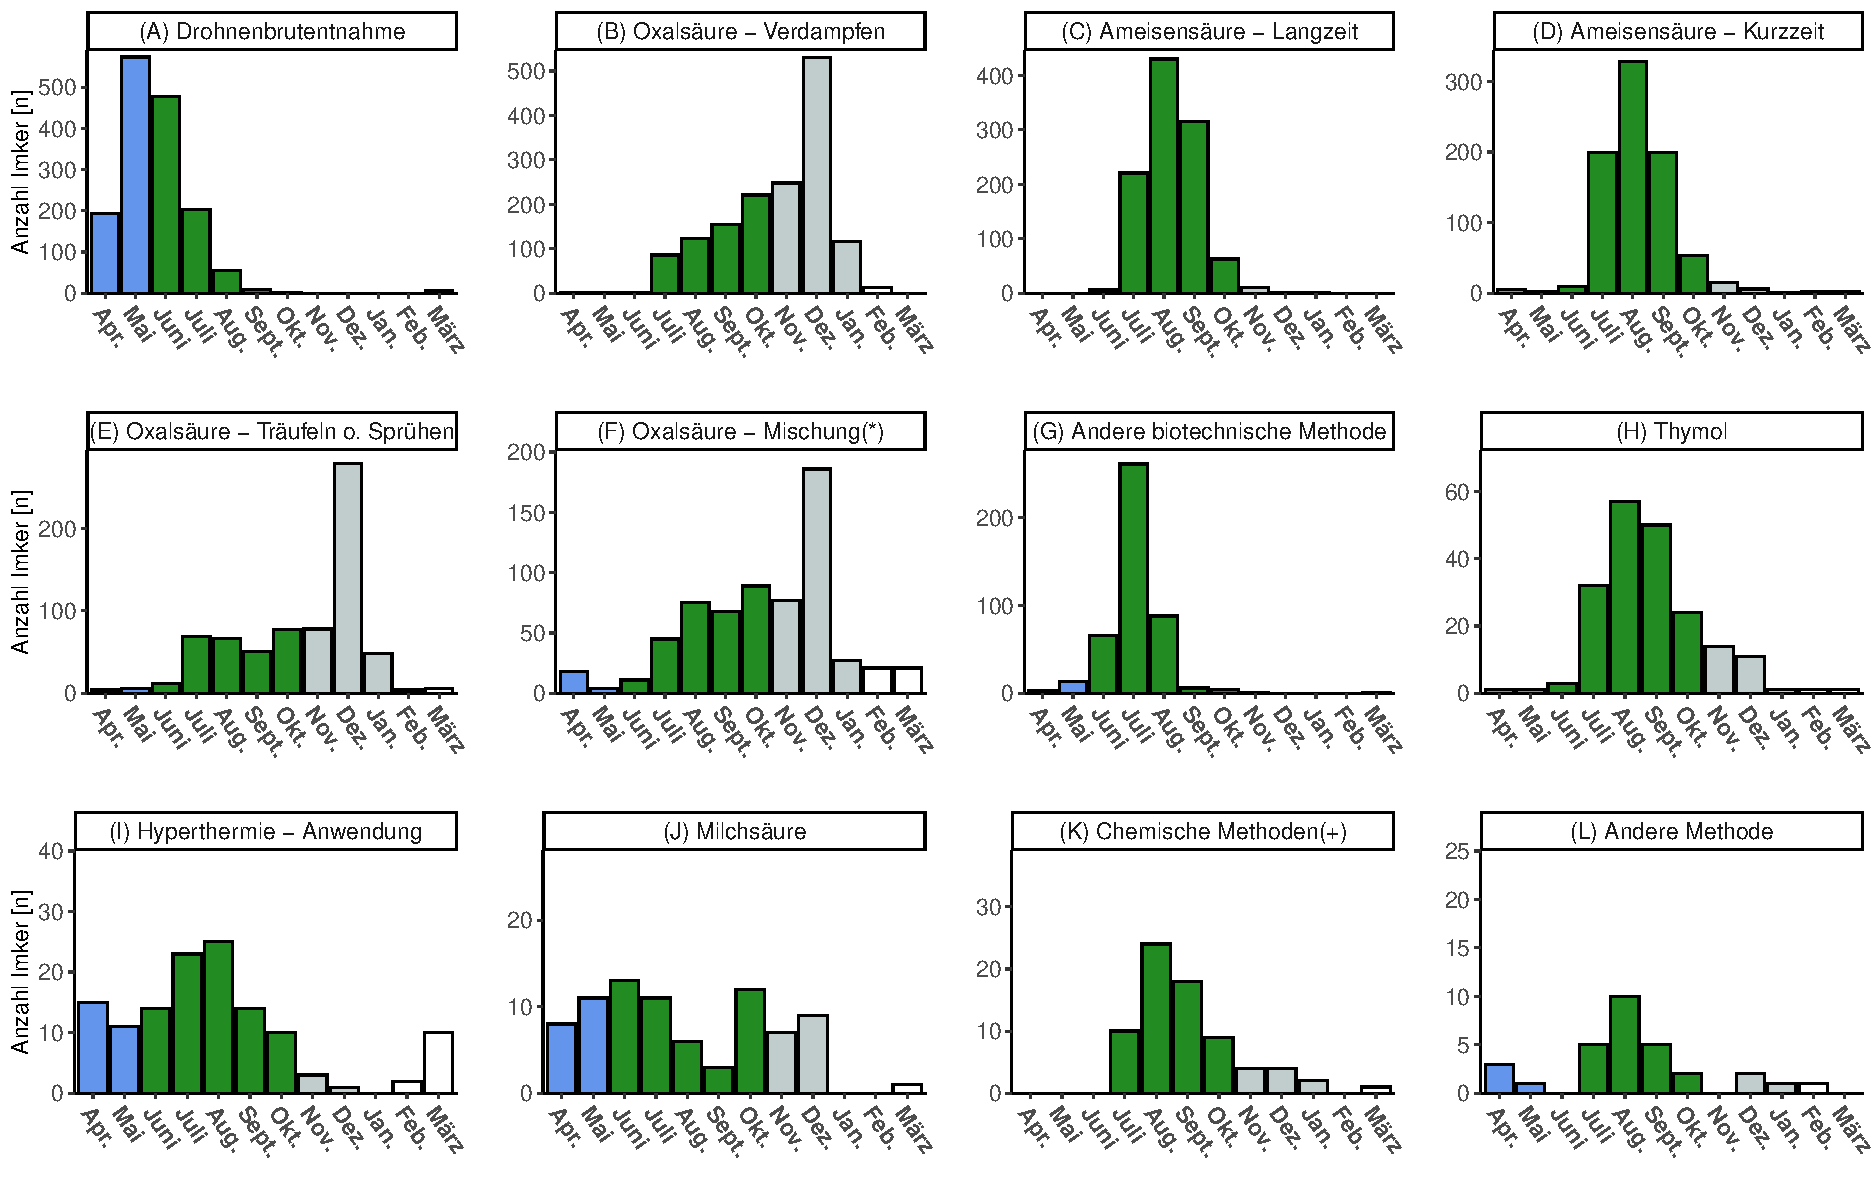
\includegraphics[keepaspectratio,width=1\textwidth]{project-U-wintersterblichkeit/figures/plot_treatment_histogramm}
  \caption{Zusammenfassung der zur Bekämpfung der Varroamilbe angewandten Methoden für das Untersuchungsjahr 2019/20 in den einzelnen Monaten. Y-Axis mit separaten Skalen für die verschiedenen Behandlungsmethoden. April-Mai wurde als Frühjahr definiert (blau), Juni-Oktober als Sommer (grün) und November-Jänner als Herbst/Winter (grau). Die Monate Februar, März 2020 (weiß) sind in der folgenden Winter-Verlustanalyse nicht inkludiert. 
  \newline 
  (+) Amitraz (Verdampfen und in Streifen, Apivar, Apitraz), Coumaphos (Checkmite+), Coumaphos (Perizin), Flumethin (Bayvarol), Tau-fluvalinat (Apistan), anderes chemisches Produkt  
  \newline 
  (*) Hiveclean, Bienenwohl, Varromed}
  \label{fig:u:treatment:histogramm}
\end{figure}

\subsubsubsection{Anwendungen in den Jahreszeiten}

Die Verlustrate und statistische Ergebnisse bei Anwendung der einzelnen Behandlungsmethoden laut \cref{fig:u:treatment:spring,fig:u:treatment:summer,fig:u:treatment:winter} werden in den folgenden Unterkapiteln näher betrachtet. Mögliche Behandlungen im Frühjahr des Folgejahres (Februar, März) sind nicht inkludiert. Die \enquote{Chemischen Methoden} wurden zusammengefasst wegen der geringen Strichprobenanzahl, siehe \cref{tab:u:behandlungsmethoden}. Sowie \enquote{Oxalsäure - Träufeln o. Sprühen} und \enquote{Oxalsäure - Mischung} werden gemeinsam betrachtet, eine getrennte Analyse der zwei Methoden findet sich im Unterkapitel \ref{sss:mischungox:u} \nameref{sss:mischungox:u}.

\myfig{project-U-wintersterblichkeit/figures/plot_treatment_spring} % Pfad
{width=1\textwidth} % Größe Relativ zu Text Breite
{Höhe der Winterverluste von 2019/20 in Prozent ($\pm$95\%CI) in Abhängigkeit von der Behandlungsmethode im Frühjahr. Einzelne Monate sind nach Saison zusammengefasst, siehe \cref{fig:u:treatment:histogramm}. Statistisch signifikante Ergebnisse sind mit einem Stern (*) gekennzeichnet.
\newline
(*) Hiveclean, Bienenwohl, Varromed
} % Text unterhalb der Grafik
{Optionaler Kurz Titel} % Optional Kurz Überschrift
{fig:u:treatment:spring} % Label zum Verweisen im Text

\myfig{project-U-wintersterblichkeit/figures/plot_treatment_summer} % Pfad
{width=1\textwidth} % Größe Relativ zu Text Breite
{Höhe der Winterverluste von 2019/20 in Prozent ($\pm$95\%CI) in Abhängigkeit von der Behandlungsmethode im Sommer. Einzelne Monate sind nach Saison zusammengefasst, siehe \cref{fig:u:treatment:histogramm}. Statistisch signifikante Ergebnisse sind mit einem Stern (*) gekennzeichnet.
\newline 
(+) Amitraz (Verdampfen und in Streifen, Apivar, Apitraz), Coumaphos (Checkmite+), Coumaphos (Perizin), Flumethin (Bayvarol), Tau-fluvalinat (Apistan), anderes chemisches Produkt  
\newline
(*) Hiveclean, Bienenwohl, Varromed}
{Optionaler Kurz Titel} % Optional Kurz Überschrift
{fig:u:treatment:summer} % Label zum Verweisen im Text

\myfig{project-U-wintersterblichkeit/figures/plot_treatment_winter} % Pfad
{width=1\textwidth} % Größe Relativ zu Text Breite
{Höhe der Winterverluste von 2019/20 in Prozent ($\pm$95\%CI) in Abhängigkeit von der Behandlungsmethode im Winter. Einzelne Monate sind nach Saison zusammengefasst, siehe \cref{fig:u:treatment:histogramm}. Statistisch signifikante Ergebnisse sind mit einem Stern (*) gekennzeichnet.
\newline 
(*) Hiveclean, Bienenwohl, Varromed}
{Optionaler Kurz Titel} % Optional Kurz Überschrift
{fig:u:treatment:winter} % Label zum Verweisen im Text

\subsubsubsection{Auswirkungen der Drohnenbrutentnahme auf die Winterverluste}
\label{sss:drohnenbrutentahme:u}

Eine der am häufigsten angewandten Methoden zur Verringerung des Varroabefalls ist die Drohnenbrutentnahme. Von den teilnehmenden Imkereien 2019/20 haben 54,3\% diese Methode in zumindest einem Monat angewandt. TeilnehmerInnen die diese Methode im Frühjahr eingesetzt haben, zeigten eine statistisch signifikant niedrigere Verlustrate (\confi{11,4}{95}{10,4}{12,4}) als TeilnehmerInnen die diese Methode nicht durchgeführt haben (\confi{13,1}{95}{12,1}{14,1}) ($\chi^{2}$=20,4, \textit{p}<0,05) (\cref{fig:u:treatment:spring}-A). Im Sommer konnte kein Unterschied zwischen den Gruppen festgestellt werden (Ja - \confi{12,3}{95}{11,1}{13,5}; Nein - \confi{12,3}{95}{11,5}{13,3}) (\cref{fig:u:treatment:summer}-A).
\newline
In weiterer Folge wurde der Zeitpunkt der Durchführung in \enquote{nur Frühling}, \enquote{nur Sommer}, die Kombination \enquote{Frühling und Sommer} sowie TeilnehmerInnern die keine Drohnenbrut entfernt haben aufgeteilt. In \cref{fig:u:treatment:drone:combination} sind die Ergebnisse grafisch dargestellt. Hier zeigt sich das die meisten TeilnehmerInnen die eine Drohnenbrutentahme durchgeführt haben diese im Frühling und Sommer gemacht haben (\sample{385}, \confi{11,3}{95}{10,1}{12,7}). Es konnte kein statistischer signifikanter Unterschied beim Zeitpunkt in den Verlustraten festgestellt werden (Nur Frühling - \confi{11,5}{95}{9,9}{13,2}; Nur Sommer - \confi{15,2}{95}{12,8}{18,0}). Auch im Vergleich zur Gruppe die keine Drohnenbrutentahme durchgeführt hat ergibt sich kein statistischer Unterschied (\confi{12,8}{95}{11,8}{14,0}). 

\myfig{project-U-wintersterblichkeit/figures/plot_treatment_drone_combination} % Pfad
{width=0.8\textwidth} % Größe Relativ zu Text Breite
{Höhe der Winterverluste von 2019/20 in Prozent ($\pm$95\%CI) in Abhängigkeit von der Behandlungsmethode \enquote{Drohnenbrutentnahme} und Zeitpunkt der Durchführung. Einzelne Monate zusammengefasst siehe \cref{fig:u:treatment:histogramm}.} % Text unterhalb der Grafik
{Optionaler Kurz Titel} % Optional Kurz Überschrift
{fig:u:treatment:drone:combination} % Label zum Verweisen im Text

Zusätzlich wurde die Auswirkung einer mehrfachen Drohnenbrutentnahme auf die Winterverluste untersucht. Das heißt ob die Anzahl der Monate, in denen eine Drohnenbrutentnahme durchgeführt wurde, einen Einfluss auf den Überwinterungserfolg hat. Dazu wurden die Verlustraten der Gruppen „0`` (=keine Behandlung) (\confi{12,8}{95}{11,8}{14,0}), „1-3 Monate`` (\confi{12,1}{95}{11,1}{13,1}) und „>3 Monate`` (\confi{11,5}{95}{8,4}{15,4}) verglichen. Bei dieser Untersuchung konnte kein signifikanter Unterschied aufgrund der Dauer der Behandlung festgestellt werden (\cref{fig:u:treatment:drone:grouped}). 

\myfig{project-U-wintersterblichkeit/figures/plot_treatment_drone_grouped} % Pfad
{width=0.6\textwidth} % Größe Relativ zu Text Breite
{Höhe der Winterverluste von 2019/20 in Prozent ($\pm$95\%CI) in Abhängigkeit von der Dauer der Drohnenbrutentnahme.} % Text unterhalb der Grafik
{Optionaler Kurz Titel} % Optional Kurz Überschrift
{fig:u:treatment:drone:grouped} % Label zum Verweisen im Text


\subsubsubsection{Ameisensäure-Behandlung}

Wir haben bei unseren Analysen zwischen Kurzzeit- und Langzeitbehandlung mit Ameisensäure unterschieden und die daraus resultierenden Verlustraten miteinander verglichen. Es ist zu vermerken, dass bei keiner der Methoden die Konzentration der verwendeten Ameisensäure abgefragt wurde.
\newline
Im Sommer zeigt sich für die Kurzzeitbehandlung kein statistischer Unterschied zwischen den ImkerInnen die diese Behandlung durchgeführt haben und denen, die sie nicht durchgeführt haben (Ja - \confi{12,8}{95}{11,7}{13,9}; Nein - \confi{12,0}{95}{11,1}{13,0}) (\cref{fig:u:treatment:summer}-D). Eine Langzeitbehandlung im Sommer führte zu statistisch signifikant niedrigeren Verlustraten (\confi{11,4}{95}{10,4}{12,5}) im Vergleich zur Gruppe die keine Langzeitbehandlung durchgeführt hat (\confi{13,0}{95}{12,1}{14,1}) ($\chi^{2}$=17,9, \textit{p}<0,05) (\cref{fig:u:treatment:summer}-E). Eine Kurzzeitbehandlung mit Ameisensäure hatte im Winter in den von uns definierten Monaten eine eine statistisch signifikante negative Auswirkung auf die Verlustraten (Ja - \confi{23,6}{95}{13,5}{37,9}; Nein - \confi{12,2}{95}{11,5}{13,0}) (\cref{fig:u:treatment:winter}-A).
\newline
Betrachtet man ImkerInnen die ausschließlich eine Kurzzeitbehandlung im Sommer durchgeführt haben, zeigen sich potentiell höhere Winterverlustraten (\confi{27,0}{95}{18,1}{38,2}) im Gegensatz zu den ImkerInnen die ausschließlich eine Langzeitbehandlung im Sommer durchgeführt haben (\confi{14,5}{95}{11,0}{19,0}) \cref{fig:u:combination}.

\subsubsubsection{Oxalsäure}

Während der Wintermonate setzen viele ImkerInnen die Oxalsäure zur Bekämpfung der Varroamilbe zur sogenannten Restentmilbung ein. Da Oxalsäure nicht in die verdeckelte Brut wirkt, muss für eine Behandlung in der warmen Jahreszeit eine Brutfreiheit gegeben sein. Alternativ kann auch eine mehrmalige Anwendung in kurzen Abständen, eine sogenannte Blockbehandlung, über den gesamten Brutzyklus eines Bienenvolkes erfolgen. 
\newline
Die Oxalsäure kann entweder durch Träufeln oder durch Verdampfen eingesetzt werden. Hiveclean, Bienenwohl und Varromed sind
kommerziell erhältliche Fertigmischungen aus Oxalsäure, Zucker und anderen Stoffen, die ebenfalls geträufelt werden. Es wurde untersucht, ob sich die Winterverlustraten bei ImkerInnen, die eine dieser Methoden eingesetzt haben, von jenen, die diese Methoden nicht angewandt haben, unterscheiden, siehe \cref{tab:u:oxal}.
\newline
Betriebe die im Frühjahr \enquote{Oxalsäure durch Träufeln o. Sprühen (inkl. Fertigmischungen)} eingesetzt haben bzw. nicht eingesetzt haben, zeigten keine statistisch signifikanten Unterschiede in den Winterverlustraten (Ja - \confi{12,8}{95}{9,0}{17,8}; Nein - \confi{12,3}{95}{11,6}{13,0}) (\cref{fig:u:treatment:spring}-C). Auch in den anderen zwei Jahreszeiten zeigte die Methode zwischen Anwendung und Nicht-Anwendung keinen signifikanten Unterschied: Sommer (Ja - \confi{12,6}{95}{11,3}{14,0}; Nein - \confi{12,2}{95}{11,4}{13,1}) (\cref{fig:u:treatment:summer}-H); Winter (Ja - \confi{13,1}{95}{12,0}{14,3}; Nein - \confi{11,8}{95}{10,9}{12,7}) (\cref{fig:u:treatment:winter}-C).
\newline
Die gleiche Auswertung für \enquote{Oxalsäure Verdampfen} zeigt im Sommer keinen signifikanten Unterschied in den Verlustraten (Ja - \confi{11,8}{95}{10,5}{13,3}; Nein - \confi{12,5}{95}{11,7}{13,3}) (\cref{fig:u:treatment:summer}-G). Im Winter zeigt sich eine signifikant niedrigere Verlustrate für das Oxalsäureverdampfen mit \confi{11,5}{95}{10,6}{12,5} als für TeilnehmerInnen die nicht verdampft haben mit \confi{13,2}{95}{12,1}{14,3} ($\chi^{2}$=18,3, \textit{p}<0,05) (\cref{fig:u:treatment:winter}-B). Eine ausschließliche Behandlung mit Oxalsäure durch Verdampfung wurde von \sample{36} TeilnehmerInnen durchgeführt und führte zu Verlustraten die im österreichischen Durchschnitt liegen (\confi{13,2}{95}{9,5}{17,9}) (\cref{fig:u:combination}-F).

\begin{table}[H]
    \centering
    \caption{Stichprobenanzahl und Verlustraten ($\pm$95\%CI) der Oxalsäure Anwendung. Einzelne Monate sind nach Saison zusammengefasst, siehe \cref{fig:u:treatment:histogramm}. $^*$Oxalsäure durch Träufeln o. Sprühen (inkl. Fertigmischungen)}    
    \begin{tabular}{lrrrr}
        \toprule
            \multicolumn{1}{c}{Anwendung} & 
            \multicolumn{2}{c}{Ja} & 
            \multicolumn{2}{c}{Nein} \\
        \cmidrule{2-5}
            \multicolumn{1}{c}{Oxalsäure} & 
            \makecell{\textit{n}} & \makecell{{Verlust (95\% KI)}} & \makecell{\textit{n}} & \makecell{{Verlust (95\% KI)}} \\
        \midrule
        Träufel$^*$ - Frühjahr &  31 & 12,8  \:\:(9,0-17,8) & 1398 & 12,3 (11,6-13,0) \\
        Träufel$^*$ - Sommer   & 363 & 12,6 (11,3-14,0) & 1066 & 12,2 (11,4-13,1) \\
        Träufel$^*$ - Winter   & 603 & 13,1 (12,0-14,3) &  826 & 11,8 (10,9-12,7) \\
        Verdampfen - Sommer    & 363 & 11,8 (10,5-13,3) & 1066 & 12,5 (11,7-13,3) \\
        Verdampfen - Winter    & 603 & 11,5 (10,6-12,5) &  826 & 13,2 (12,1-14,3) \\
        \bottomrule
    \end{tabular}
    \label{tab:u:oxal}
\end{table}

\subsubsubsection{Hiveclean/Bienenwohl/Varromed}
\label{sss:mischungox:u}

Kommerzielle Oxalsäure-Fertigmischungen mit dem Wirkstoff Oxalsäure (und weiteren Hilfsstoffen) werden für einen guten Behandlungserfolg im brutfreien Volk eingesetzt. Im Untersuchungsjahr 2019/20 setzten 26,9\% aller befragten ImkerInnen eines dieser Produkte zur Bekämpfung der Varroamilbe ein. Es konnte kein signifikanter Unterschied in der Verlustrate beobachtet werden, wenn eine Fertigmischung zur Bekämpfung der Varroamilbe verwendet wurde mit \confi{12,9}{95}{11,4}{14,6} oder reine Oxalsäure geträufelt wurde \confi{12,8}{95}{11,5}{14,2}.
Auch wenn beides verwendet wurde (\confi{11,8}{95}{9,3}{14,8}) oder keine der beiden Methoden \confi{11,8}{95}{10,8}{12,9} führte es zu keinen statistisch signifikanten Unterschieden \cref{fig:u:treatment:oxalmix}.

\begin{figure}[H]
  \centering
  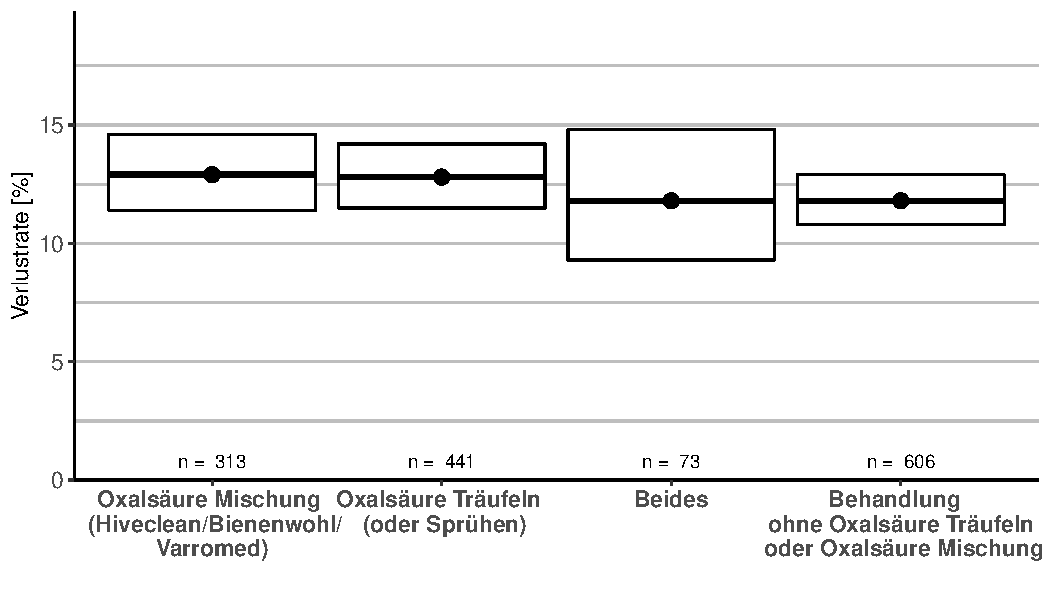
\includegraphics[keepaspectratio,width=0.8\textwidth]{project-U-wintersterblichkeit/figures/plot_treatment_oxalmix}
  \caption{Höhe der Winterverluste von 2019/20 in Prozent ($\pm$95\%CI) in Abhängigkeit von der Varroabekämpfung mit einer Oxalsäure-Fertigmischung (Hiveclean, Bienenwohl, Varromed) zu reiner Oxalsäure-Lösung, in Kombination und ohne die zwei Methoden.}
  \label{fig:u:treatment:oxalmix}
\end{figure}

\subsubsubsection{Thymol}

Von 7,7\% aller befragten ImkerInnen wurde angegeben, eine Behandlung mit Thymol durchgeführt zu haben. Hierbei zeigt sich für Betriebe die im Sommer Thymol eingesetzt haben eine statistisch signifikant höhere Verlustrate mit \confi{18,4}{95}{14,9}{22,4} als für die Gruppe die kein Thymol eingesetzt hat \confi{12,0}{95}{11,3}{12,7} (\cref{fig:u:treatment:summer}-I).
\newline
Betrachtet man die Häufigkeit der Anwendungen in Monaten im Vergleich zu den Winterverlusten, zeigten sich für ImkerInnen mit einmaliger Anwendung statistisch signifikant höhere Verlustraten mit \confi{22,4}{95}{17,4}{28,3} im Vergleich zu keiner Thymol-Behandlung mit \confi{12,3}{95}{11,6}{13}. TeilnehmerInnen die in mehr als einem Monat mit Thymol behandelt haben, zeigen keinen statistisch signifikanten Unterschied \confi{13,9}{95}{9,8}{19,3} (\cref{fig:u:treatment:thymol:grouped}).

\begin{figure}[H]
  \centering
  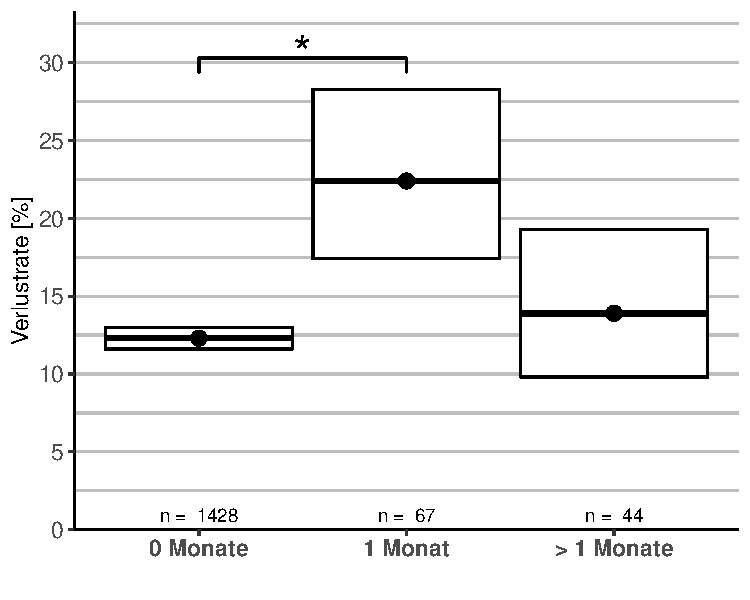
\includegraphics[keepaspectratio,width=0.7\textwidth]{project-U-wintersterblichkeit/figures/plot_treatment_thymol_grouped}
  \caption{Höhe der Winterverluste 2019/20 in Prozent (\(\pm\)95\%CI) in Abhängigkeit von der Häufigkeit der Anwendungen in Monaten von Produkten auf Thymolbasis. Statistisch signifikante Ergebnisse sind mit einem Stern (*) gekennzeichnet.}
  \label{fig:u:treatment:thymol:grouped}
\end{figure}

\subsubsubsection{Hyperthermie}

Eine Alternative zur chemischen Behandlung der Völker gegen die Varroamilbe stellt die Hitzebehandlung (=Hyperthermie) dar. Sie beruht auf der unterschiedlichen Wärmetoleranz von Bienen und Milben. 4,6\% der ImkerInnen, die sich an der Erhebung der Winterverluste beteiligt haben, wendeten diese nicht-chemische Behandlung in zumindest einem Monat an. Es wurde nicht zwischen den verschiedenen am Markt erhältlichen Systemen zur Hitzebehandlung unterschieden. Hinsichtlich der Verlustrate fanden wir keine statistisch signifikanten Unterschiede zwischen Imkereien, die mit Hyperthermie behandelt haben und jenen, die nicht damit behandelt haben: Frühjahr (Ja - \confi{12,8}{95}{8,8}{18,2}; Nein - \confi{12,3}{95}{11,6}{13,0}); Sommer (Ja - \confi{11,9}{95}{9,0}{15,6}; Nein - \confi{12,3}{95}{11,6}{13,1}) (\cref{fig:u:treatment:spring}, \cref{fig:u:treatment:summer} - B).

\newpage 

\subsubsubsection{Andere biotechnische Methoden (ohne Hyperthermie /  Drohnenbrutentnahme)}

Andere biotechnische Methoden, mit Ausnahme von Hyperthermie und Drohnenbrutentnahme, wurden zusammengefasst abgefragt. 25,7\% der befragten ImkerInnen gaben an eine solche biotechnische Methode angewendet zu haben. Dazu zählen die Verwendung von Fangwaben oder Bannwaben oder die totale Brutentnahme.
\newline
Im Untersuchungsjahr 2019/20 zeigten sich signifikant niedrigere Verlustraten bei einer Anwendung dieser Methode im Sommer (Ja - \confi{11,2}{95}{10,1}{12,3}; Nein - \confi{13,0}{95}{12,1}{13,9}; $\chi^{2}$=21,1, \textit{p}<0,05) (\cref{fig:u:treatment:summer} - C).

\subsubsubsection{Behandlungskombinationen}
\label{sss:kombination:U}

Die diversen Kombinationen (\cref{fig:u:combination}) beinhalten alle möglichen Kombinationen der Behandlungen nach Jahreszeiten mit mindestens 15 ImkerInnen, ohne Drohnenbrutentnahme. Eine Risikoanalyse zur Drohnenbrutentahme wurde extra angeführt und ausgewertet (siehe \ref{sss:drohnenbrutentahme:u} \nameref{sss:drohnenbrutentahme:u}). Im Untersuchungsjahr 2019/20 gab es insgesamt 332 unterschiedlichen Behandlungskombinationen. Es wurden statistisch nur die Kombinationen ausgewertet die von mindestens 15 TeilnehmerInnen durchgeführt wurden. Dieser Filter führte zu 19 verschiedenen Kombinationen und ihren jeweiligen Verlustraten (\cref{fig:u:combination}, \cref{tab:u:kombinationen}). Hierbei sei bei den Kombinationen mit kleineren Stichproben auf die breiten Konfidenzintervalle hingewiesen.
\newline
Die Kombination mit den meisten TeilnehmerInnen war die Langzeitbehandlung mit Ameisensäure im Sommer gefolgt von Oxalsäure mittels Träufeln im Winter (\sample{138}, \confi{10,1}{95}{8,2}{12,5}, (A)) beziehungsweise Sublimation der Oxalsäure im Winter (\sample{88}, \confi{ 11,1}{95}{ 8,7}{ 14,0}, (B)). Ein signifikante höhere Verlustrate im Vergleich zum österreichischen Durchschnitt hatten TeilnehmerInnen die nur eine Ameisensäure - Kurzzeitbehandlung im Sommer durchgeführt haben \confi{27,0}{95}{18,1}{38,2} (L). 
\newline
Biotechnische Maßnahmen im Sommer gefolgt von Oxalsäure im Sommer und Winter zeigt ein Potential für niedrigere Verlustraten gegenüber dem österreichische Durchschnitt ((E) - \confi{11,1}{95}{8,5}{14,4}; (Q) - \confi{9,2}{95}{5,4}{15,1}; (P) - \confi{9,0}{95}{5,6}{14,3}).

\myfig{project-U-wintersterblichkeit/figures/plot_combination_loss_new} % Pfad
{width=1\textwidth} % Größe Relativ zu Text Breite
{Höhe der Winterverluste von 2019/20 in Prozent ($\pm$95\%CI) in Abhängigkeit von der Behandlungsmethodenkombination und dem Zeitpunkt der Durchführung. Einzelne Monate zusammengefasst siehe \cref{fig:u:treatment:histogramm}. Nur Kombinationen von Methoden mit mindestens 15 TeilnehmerInnen wurden ausgewertet. Die Anzahl der unterschiedlichen Behandlungsmethoden ist farblich gekennzeichnet (weiß = 1, grau = 2, schwarz = 3). Der österreichischer Durchschnitt (rote Linie) mit ($\pm$95\%CI) (gestrichelte Linie) ist vertikal eingezeichnet. Abkürzungen der Behandlungsmethoden siehe \cref{tab:u:kombinationen}.} % Text unterhalb der Grafik
{Optionaler Kurz Titel} % Optional Kurz Überschrift
{fig:u:combination} % Label zum Verweisen im Text

\newpage
\begin{landscape}

\begin{table}[H]
  \centering
  \caption{Verlustraten und Stichprobenanzahl der Kombinationen. W = Winter, S = Sommer, Einzelne Monate sind nach Saison zusammengefasst, siehe \cref{fig:u:treatment:histogramm}.}
  \scriptsize
  \setlength{\tabcolsep}{0.5em} % for the horizontal padding
  \label{tab:u:kombinationen}
  \begin{tabular}{l|*{6}{l}|rr}
  \toprule
    \multicolumn{1}{c|}{Abkürzung} & 
    \multicolumn{6}{c|}{Methode} & 
    \multicolumn{1}{c}{\textit{n}} &
    \multicolumn{1}{c}{Verlust (95\% CI)}
    \\
    \midrule
    (A) S-AS-LZ \& W-Ox-Träu. & S & Ameisensäure - Langzeit & W & Oxalsäure - träufeln & & & 138 & 10,1 (8,2-12,5) \\
    (B) S-AS-LZ \& W-Ox-Sub.  & S & Ameisensäure - Langzeit & W & Oxalsäure - sub.     & & & 88  & 11,1 (8,7-14) \\
    (C) S-AS-KZ \& W-Ox-Träu. & S & Ameisensäure - Kurzzeit & W & Oxalsäure - träufeln & & & 61  & 12,1 (9,4-15,4) \\
    (D) S-AS-LZ               & S & Ameisensäure - Langzeit &        &                      & & & 57  & 14,5 (11,0-19,0) \\
    (E) S-Biot. \& S-Ox-Sub. \& W-Ox-Sub. & S & Andere biotechnische Methode & S & Oxalsäure - sub. & W & Oxalsäure - sub. & 53 & 11,1 (8,5-14,4) \\
    (F) S-AS-KZ \& S-AS-LZ \& W-Ox-Träu. & S & Ameisensäure - Kurzzeit      & S & Ameisensäure - Langzeit & W & Oxalsäure - träufeln & 46 & 14,5 (10,3-20,1) \\
    (G) S-AS-KZ \& W-Ox-Sub.                & S & Ameisensäure - Kurzzeit & W & Oxalsäure - sub.     & & & 36 & 16,0 (11,3-22) \\
    (H) S-Ox-Sub. \& W-Ox-Sub.              & S & Oxalsäure - sub.        & W & Oxalsäure - sub.     & & & 36 & 13,2 (9,5-17,9) \\
    (I) S-AS-LZ \& S-Ox-Sub. \& W-Ox-Sub.   & S & Ameisensäure - Langzeit & S & Oxalsäure - sub. & W & Oxalsäure - sub. & 34 & 13,3 (9,0-19,3) \\
    (J) S-AS-KZ \& S-AS-LZ \& W-Ox-Sub. & S & Ameisensäure - Kurzzeit & S & Ameisensäure - Langzeit & W & Oxalsäure - sub. & 31 & 12,2 (7,7-18,8) \\
    (K) S-AS-KZ \& S-Ox-Sub. \& W-Ox-Sub. & S & Ameisensäure - Kurzzeit & S & Oxalsäure - sub. & W & Oxalsäure - sub. & 27 & 11,7 (8,3-16,4) \\
    (L) S-AS-KZ                            & S & Ameisensäure - Kurzzeit &  &  &  & & 23 & 27,0 (18,1-38,2) \\
    (M) S-AS-LZ \& S-Ox-Träu. \& W-Ox-Träu. & S & Ameisensäure - Langzeit & S & Oxalsäure - träufeln & W & Oxalsäure - träufeln & 23 & 12,7 (8,7-18,2) \\
    (N) S-AS-KZ \& S-Ox-Träu. \& W-Ox-Träu. & S & Ameisensäure - Kurzzeit & S & Oxalsäure - träufeln & W & Oxalsäure - träufeln & 21 & 15,1 (10-22,2) \\
    (O) S-Biot. \& S-AS-LZ \& W-Ox-Träu. & S & Andere biotechnische Methode & S & Ameisensäure - Langzeit & W & Oxalsäure - träufeln & 20 & 13,8 (9,6-19,4) \\
    (P) S-Biot. \& S-Ox-Träu. \& W-Ox-Träu. & S & Andere biotechnische Methode & S & Oxalsäure - träufeln & W & Oxalsäure - träufeln & 19 & 9,2 (5,4-15,1) \\
    (Q) S-Biot. \& S-Ox-Träu.   \& W-Ox-Sub. & S & Andere biotechnische Methode & S & Oxalsäure - träufeln & W & Oxalsäure - sub. & 18 & 9,0 (5,6-14,3) \\
    (R) S-AS-LZ \& S-Ox-Träu. \& W-Ox-Sub. & S & Ameisensäure - Langzeit & S & Oxalsäure - träufeln & W & Oxalsäure - sub. & 17 & 13,8 (8,1-22,6) \\
    (S) S-AS-KZ \& S-Ox-Träu. \& W-Ox-Sub. & S & Ameisensäure - Kurzzeit & S & Oxalsäure - träufeln & W & Oxalsäure - sub. & 16 & 15,1 (8,0-26,7) \\
    \bottomrule
\end{tabular}
\end{table}

\end{landscape}
\newpage

\subsubsection{Königinnen-Verluste}
\label{ss:koeniginnen_verluste:U}

Die Winterverlustrate durch \enquote{Unlösbare Königinnenprobleme} für ganz Österreich lag 2019/20 bei \confi{4,3}{95}{4,1}{4,6}. Der Vergleich von Bundesländern zur österreichischen Gesamt-Verlustrate zeigt keinen statistisch signifikanten Unterschied. Zwischen den Bundesländern zeigt sich für Niederösterreich eine signifikant höhere Verlustrate mit \confi{5,0}{95}{4,5}{5,6} im Vergleich zu Vorarlberg mit \confi{3,1}{95}{2,3}{4,3}.
\newline
Die Verlustraten der anderen Bundesländer ergeben: Burgenland \confi{4,4}{95}{2,7}{7,0}; Kärnten \confi{3,7}{95}{3,1}{4,5}; Oberösterreich \confi{4,6}{95}{4,0}{5,3}; Salzburg \confi{4,4}{95}{3,2}{5,9}; Steiermark \confi{3,9}{95}{3,3}{4,6}; Tirol \confi{4,0}{95}{3,3}{4,8} und Wien \confi{4,5}{95}{3,3}{6,1} \cref{fig:u:queen:states}.

\begin{figure}[H]
  \centering
  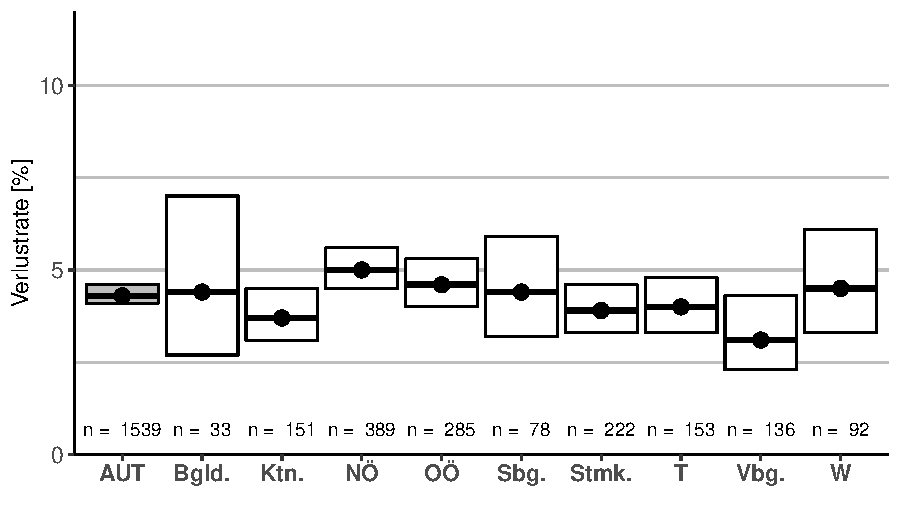
\includegraphics[keepaspectratio,width=0.8\textwidth]{project-U-wintersterblichkeit/figures/plot_queen_states}
  \caption{Höhe der Winterverluste 2019/20 durch unlösbare Königinnenprobleme verursacht für die einzelnen Bundesländer und Österreich gesamt in Prozent ($\pm$95\%CI).}
  \label{fig:u:queen:states}
\end{figure}

\subsubsubsection{Königinnenprobleme}
\label{ss:koeniginnen_probleme:U}

Die Überlebenschance der Völker hängt in großem Maße auch von der Gesundheit der Königin ab. Die Imkereien wurden deshalb auch über das Auftreten von Königinnenproblemen befragt und konnten zwischen den vier Antworten „Häufiger``, „Normal``, „Seltener`` und „Weiß nicht`` (im Vergleich zu den Vorjahren) entscheiden. \cref{tab:u:queenproblems} zeigt die Angaben der TeilnehmerInnen seit 2013/14.
\newline
TeilnehmerInnen die diese Probleme \enquote{Häufiger} beobachteten hatten signifikant höhere Verluste durch \enquote{Unlösbare Königinnenprobleme} mit \confi{6,8}{95}{5,8}{7,9} im Vergleich zu den anderen Gruppen: Normal - \confi{4,3}{95}{4,0}{4,8}, Seltener - \confi{3,7}{95}{3,2}{4,2}, Weiß nicht - \confi{3,8}{95}{2,8}{5,0} (\cref{fig:u:queen:problems}-A). Auch bei den Winterverlusten (exklusive \enquote{Unlösbare Königinnenprobleme}) zeigte sich derselbe Trend mit signifikant höheren Verlusten für \enquote{Häufiger} mit \confi{11,2}{95}{8,9}{14,0} im Vergleich zu den anderen Gruppen: Normal - \confi{7,1}{95}{6,2}{8,1}; Seltener - \confi{7,4}{95}{6,2}{8,7}. Nur die Gruppe \enquote{Weiß nicht} zeigte hier keinen signifikanten Unterschied mit \confi{10,8}{95}{7,9}{14,5} (\cref{fig:u:queen:problems}-B).

\begin{table}[H]
    \centering
    \caption{Art der Teilnahme an der Erhebung der Winterverluste von 2013/14 bis 2019/20 (Anzahl TeilnehmerInnen (\%)).}
    \label{tab:u:queenproblems}
    \begin{tabular}{c|*{3}{rr|}*{2}{r}}
        %\hline
            \multicolumn{1}{c}{} & 
            \multicolumn{2}{c|}{Häufiger} & 
            \multicolumn{2}{c|}{Normal} & 
            \multicolumn{2}{c|}{Seltener} &
            \multicolumn{2}{c}{Weiß nicht}
            \\
        \cline{2-9}
            \multicolumn{1}{c}{Jahr} & 
            \multicolumn{1}{c}{\textit{n}} & 
            \multicolumn{1}{c|}{\%} & 
            \multicolumn{1}{c}{\textit{n}} & 
            \multicolumn{1}{c|}{\%} & 
            \multicolumn{1}{c}{\textit{n}} & 
            \multicolumn{1}{c|}{\%} &
            \multicolumn{1}{c}{\textit{n}} & 
            \multicolumn{1}{c}{\%} \\
        \hline
     2013/14 &  76 &  8,0 & 458 & 48,1 & 212 & 22,2 & 207 & 21,7 \\
     2014/15 & 194 & 16,6 & 513 & 44,0 & 181 & 15,5 & 279 & 23,9 \\
     2015/16 &  63 &  5,2 & 491 & 40,7 & 399 & 33,1 & 253 & 21,0 \\
     2016/17 & 160 & 10,2 & 743 & 47,4 & 396 & 25,2 & 272 & 17,3 \\
     2017/18 &  72 &  6,6 & 529 & 48,4 & 332 & 30,3 & 162 & 14,8 \\
     2018/19 &  95 &  6,2 & 587 & 38,3 & 389 & 25,4 & 463 & 30,2 \\
     2019/20 & 127 & 10,4 & 570 & 46,9 & 354 & 29,1 & 165 & 13,6 \\
     \hline
    \end{tabular}
\end{table}

\begin{figure}[H]
  \centering
  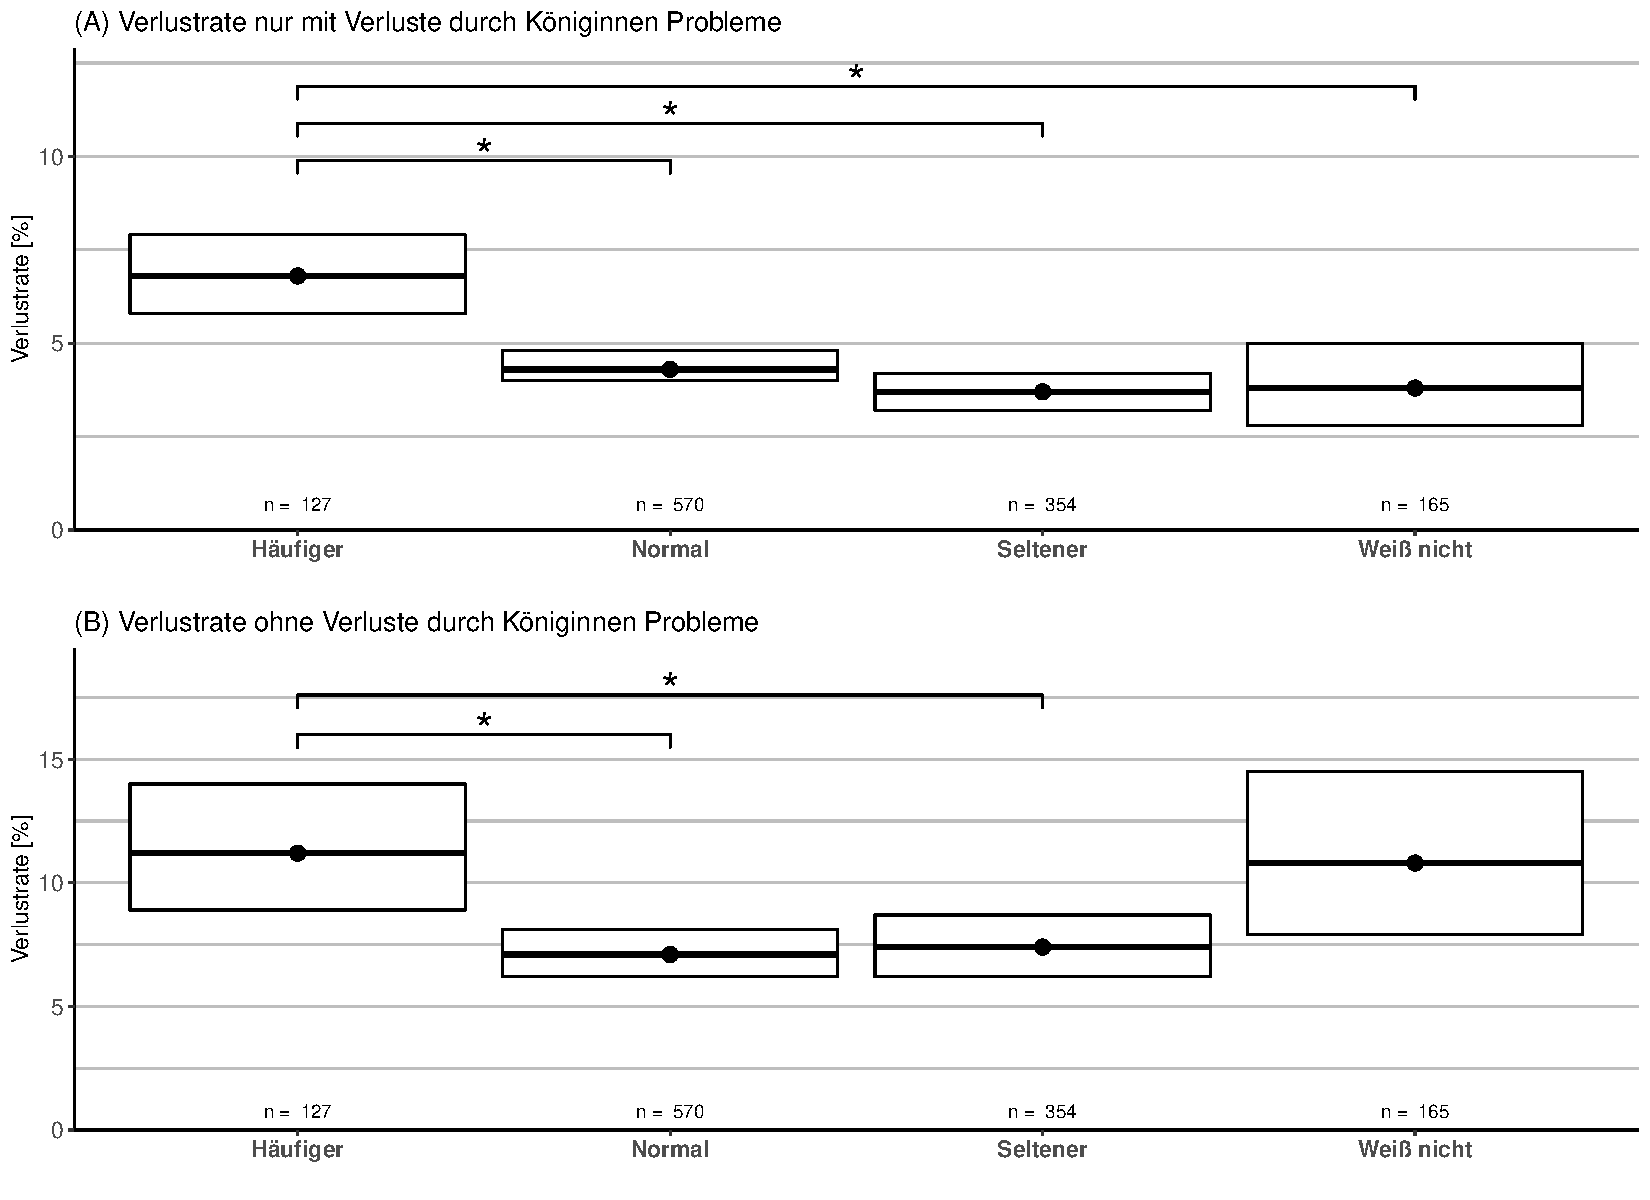
\includegraphics[keepaspectratio,width=0.9\textwidth]{project-U-wintersterblichkeit/figures/plot_queen_subjectiveproblems}
  \caption{Höhe der Winterverluste 2019/20 im Zusammenhang mit den beobachteten Königinnenproblemen in Prozent ($\pm$95\%CI). (A) nur Verluste durch unlösbare Königinnenprobleme. (B) Winterverluste exklusive den Verlusten durch unlösbare Königinnenprobleme. Statistisch signifikante Ergebnisse sind mit einem Stern (*) gekennzeichnet.}
  \label{fig:u:queen:problems}
\end{figure}


\subsubsubsection{Im Einwinterungsjahr begattete Königin (\enquote{junge Königin})}
\label{ss:junge_koeniginnen:U}

Die ImkerInnen wurden nach der Anzahl ihrer Völker mit junger Königin befragt, um zu sehen, ob sich die Überlebenschancen von Völkern mit einer jungen, das heißt im Jahr 2019 begatteten Königin, im Vergleich zu Völkern mit einer älteren Königin unterscheiden. Hier gab sich in unserer Umfrage ein Anteil an jungen Königinnen von 53,1\% in Österreich. Zur Berechnung des Anteils an jungen Königinnen wurden nur TeilnehmerInnen herangezogen welche die Frage \enquote{Wie viele Ihrer eingewinterten Völker hatten eine im Jahr 2019 begattete („junge``) Königin?} beantwortet haben.
\newline
Beim Vergleich der Austauschraten mit Verlusten durch \enquote{Unlösbare Königinnenprobleme} zeigt sich kein signifikanter Unterschied zwischen den Gruppen: 0-25\% (\confi{4,0}{95}{3,1}{5,1}); 26-50\% (\confi{4,4}{95}{3,9}{4,8}); 51-75\% (\confi{4,6}{95}{4,2}{5,1}) und 76-100\% (\confi{3,8}{95}{3,2}{4,6}) (\cref{fig:u:queen:exchangerate} - A).
\newline
Ein signifikant positiver Effekt mit weniger Verlusten bei mehr eingesetzten jungen Königinnen zeigt sich aber für die Verlustraten exklusive \enquote{Unlösbare Königinnenprobleme}. Hier zeigt die Gruppe in der nur \enquote{0-25\%} Königinnen getauscht wurden statistisch signifikant höhere Verlustraten mit \confi{15,3}{95}{12,4}{18,8} im Gegensatz zu den Gruppen in denen prozentual mehr junge Königinnen eingesetzt wurden \enquote{26-50\%} (\confi{8,8}{95}{7,8}{9,9}); \enquote{51-75\%} (\confi{6,0}{95}{5,1}{7,0}) und \enquote{76-100\%} (\confi{8,0}{95}{6,4}{10,0}). Zusätzlich hat die Gruppe \enquote{26-50\%} statistisch signifikant höhere Verlustraten als die Gruppe \enquote{51-75\%} (\cref{fig:u:queen:exchangerate} - B).

\begin{figure}[H]
  \centering
  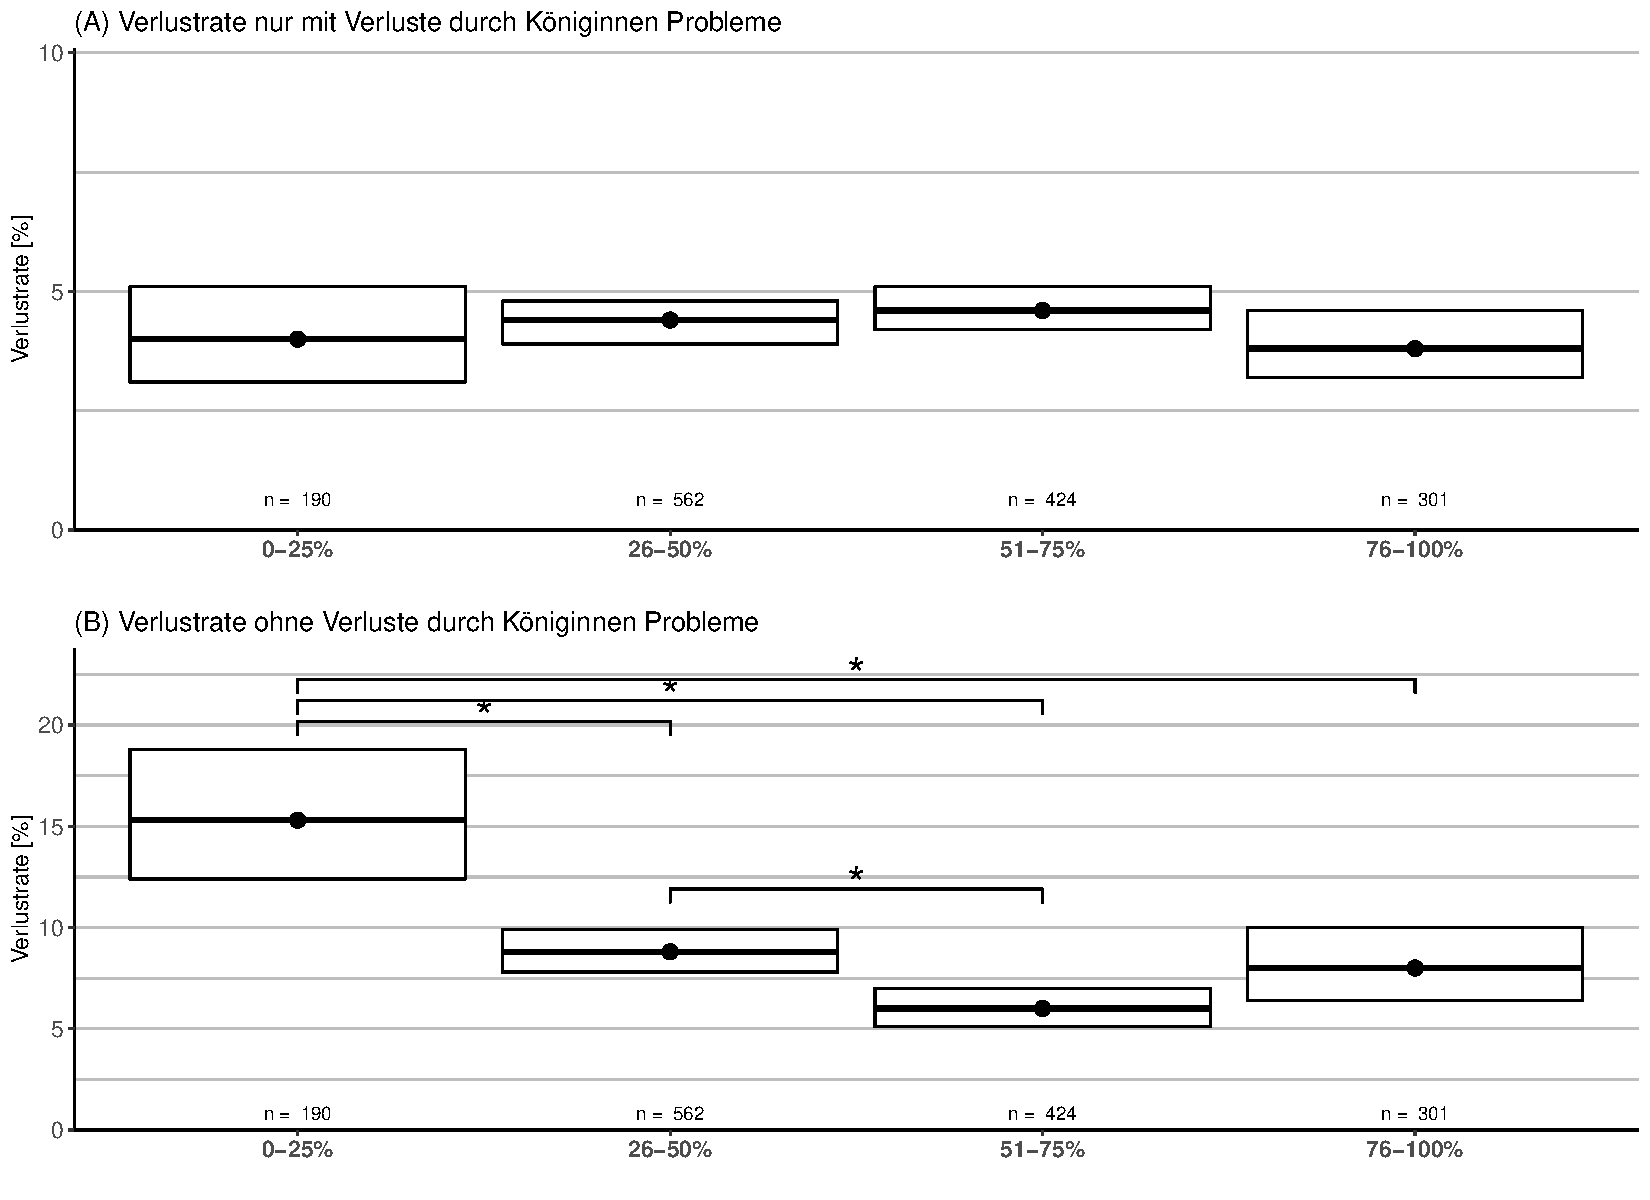
\includegraphics[keepaspectratio,width=0.9\textwidth]{project-U-wintersterblichkeit/figures/plot_queen_exchangerate}
  \caption{Höhe der Winterverluste 2019/20 in Prozent ($\pm$95\%CI) in Abhängigkeit vom Prozentsatz junger Königinnen pro Imkerei. (A) nur Verluste durch unlösbare Königinnenprobleme. (B) Winterverluste exklusive den Verlusten durch unlösbare Königinnenprobleme. Statistisch signifikante Ergebnisse sind mit einem Stern (*) gekennzeichnet.}
  \label{fig:u:queen:exchangerate}
\end{figure}

\subsubsection{Verkrüppelte Flügel}
\label{ss:verkeuppelte_fluegel:U}

In der Erhebung 2019/20 wurde nach dem Auftreten von Bienen mit verkrüppelten Flügeln während der Sammelsaison 2019 gefragt. Nur 2,0\% der Imkereien beobachtete diese \enquote{Häufig}, die Gruppe hatte aber eine statistisch signifikant höhere Verlustrate mit \confi{19,4}{95}{15,3}{24,3} im Vergleich zur Gruppe \enquote{Wenig} mit \confi{12,6}{95}{11,5}{13,8} sowie wenn verkrüppelte Flügel \enquote{Überhaupt nicht} beobachtet wurden mit \confi{11,5}{95}{10,6}{12,5}. Keinen signifikanten Unterschied gab es zu den Gruppen \enquote{Weiß nicht} mit \confi{17,3}{95}{12,3}{23,7} und \enquote{keine Angaben} mit \confi{14,0}{95}{9,3}{20,4} (\cref{fig:u:queen:crippledbees}).

\begin{figure}[H]
  \centering
  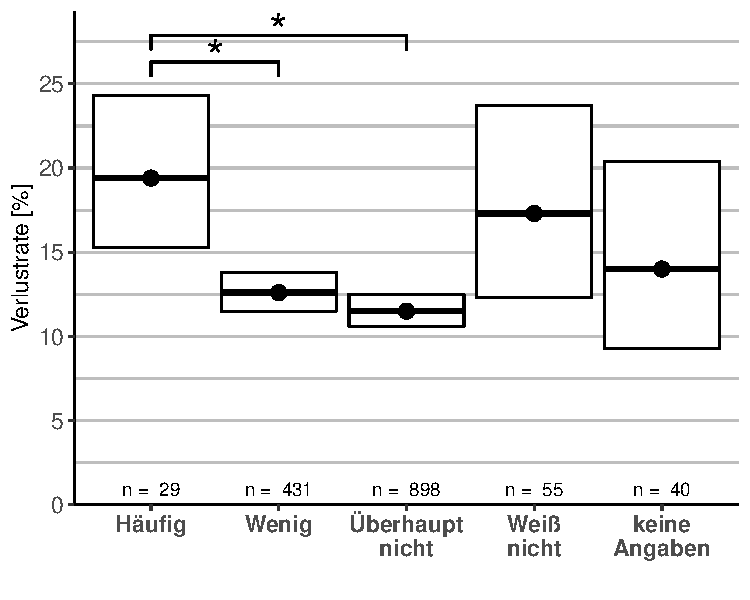
\includegraphics[keepaspectratio,width=0.6\textwidth]{project-U-wintersterblichkeit/figures/plot_factor_crippledbees}
  \caption{Höhe der Winterverluste 2019/20 in Prozent ($\pm$95\%CI) in Abhängigkeit von der Angabe wie häufig während der Sammelsaison 2019 Bienen mit verkrüppelten Flügeln in den Völkern bemerkt wurden. Statistisch signifikante Ergebnisse sind mit einem Stern (*) gekennzeichnet.}
  \label{fig:u:queen:crippledbees}
\end{figure}
\section{Diskussion}

\blindtext

\section{Anhang}

\begin{table}[H]
    \centering
    \caption{Burgenland - Jahresvergleich der Verlustraten in den Bezirken. Verlustrate in \%, (TeilnehmerInnen; eingewinterte Völker). -: weniger als fünf TeilnehmerInnen.}
    \scriptsize
    \setlength{\tabcolsep}{0.5em} % for the horizontal padding
    \label{tab:u:district-burgenland}
    \begin{tabular}{|c|*{5}{rr|}}
        \hline
        \multicolumn{11}{|c|}{Burgenland - Verlustrate \% (Teilnehmer, eingewinterte Völker)} \\    
        \hline
        \makecell{Jahre} & 
        \multicolumn{2}{c|}{Eisenstadt}    & 
        \multicolumn{2}{c|}{Eisenstadt-Umgebung}    & 
        \multicolumn{2}{c|}{Güssing} & 
        \multicolumn{2}{c|}{Jennersdorf}  &  
        \multicolumn{2}{c|}{Mattersburg} 
        \\
        \hline
        2013/24 & - &  &       - &         &       - &           &       - &         &       - &          \\
        2014/15 & - &  & 40,30\% & (6; 67) & 42,24\% & (13; 161) & 42,71\% & (8; 96) &       - &          \\
        2015/16 & - &  &       - &         &       - &           & 23,53\% & (5; 85) &       - &          \\
        2016/17 & - &  &       - &         & 31,46\% &   (6; 89) &       - &         & 28,93\% & (9; 121) \\
        2017/18 & - &  &       - &         &       - &           &       - &         &  9,49\% & (8; 137) \\
        2018/19 & - &  &       - &         &       - &           &       - &         & 16,30\% & (8; 135) \\
        2019/20 & - &  &       - &         &       - &           &       - &         &  8,05\% & (5;  87) \\
        \hline
        \makecell{Jahre} & 
        \multicolumn{2}{c|}{Neusiedl am See}    & 
        \multicolumn{2}{c|}{Oberpullendorf}    & 
        \multicolumn{2}{c|}{Oberwart} & 
        \multicolumn{2}{c|}{Rust}  & &  \\
        \hline
        2013/14 &       - &          &        - &          & 31,82\% &   (5; 88) & - &  &&\\
        2014/15 & 24,72\% & (7; 178) & 53,72\% & (12; 376) & 30,08\% & (17; 256) & - &  &&\\
        2015/16 &  3,55\% & (5; 169) & 20,51\% &   (7; 78) &  4,17\% &   (9;144) & - &  &&\\
        2016/17 & 12,22\% & (8; 311) & 20,95\% & (12; 253) & 27,57\% & (15; 185) & - &  &&\\
        2017/18 &  6,45\% &  (5; 62) &  5,00\% &   (5; 60) & 11,96\% &   (7; 92) & - &  &&\\
        2018/19 &  8,16\% & (7; 147) &       - &           &  5,58\% &  (9; 269) & - &  &&\\
        2019/20 &      -  &          & 15,09\% &   (7; 53) & 13,11\% &  (10;183) & - &  &&\\
        \hline
    \end{tabular}
\end{table}


\begin{table}[H]
    \centering
    \caption{Kärnten - Jahresvergleich der Verlustraten in den Bezirken. Verlustrate in \%, (TeilnehmerInnen; eingewinterte Völker). -: weniger als fünf TeilnehmerInnen.}
    \scriptsize
    \setlength{\tabcolsep}{0.5em} % for the horizontal padding
    \label{tab:u:district-kaernten}
    \begin{tabular}{|c|*{5}{rr|}}
        \hline
        \multicolumn{11}{|c|}{Kärnten - Verlustrate \% (Teilnehmer, eingewinterte Völker)} \\    
        \hline
        \makecell{Jahre} & 
        \multicolumn{2}{c|}{Feldkirchen}    & 
        \multicolumn{2}{c|}{Hermagor}    & 
        \multicolumn{2}{c|}{Klagenfurt am Wörthersee} & 
        \multicolumn{2}{c|}{Klagenfurt-Land}  &  
        \multicolumn{2}{c|}{Sankt Veit an der Glan} 
        \\
        \hline
        2013/14 & 11,39\% & (7; 202) &  5,48\% & (20; 365) & 12,66\% &   (5; 79) &  6,76\% & (10; 281) & 15,32\% & (15; 385) \\
        2014/15 & 32,46\% & (6; 191) & 56,41\% & (11; 195) & 54,55\% &  (10; 77) & 34,55\% & (18; 330) & 26,45\% & (25; 881) \\
        2015/16 &  3,86\% & (5; 233) &  5,93\% & (17; 337) & 12,10\% &  (9; 124) &  4,98\% & (15; 301) &  7,28\% & (12; 604) \\
        2016/17 & 40,11\% & (7; 187) & 19,95\% & (19; 436) & 52,43\% &  (9; 103) & 15,34\% & (10; 189) & 41,05\% & (16; 592) \\
        2017/18 & 13,99\% & (5; 193) & 14,51\% & (22; 448) & 25,79\% &  (8; 159) &  6,16\% &  (9; 276) & 20,48\% & (16; 420) \\
        2018/19 &  7,06\% & (6; 354) & 12,03\% & (18; 316) & 13,54\% & (10; 192) & 11,22\% & (16; 401) &  7,22\% & (16; 568) \\
        2019/20 &  8,81\% & (8; 318) & 11,24\% & (20; 436) &  8,86\% &   (5; 79) & 13,52\% & (21; 355) & 18,58\% & (13; 366) \\
        \hline
        \makecell{Jahre} & 
        \multicolumn{2}{c|}{Spittal an der Drau}    & 
        \multicolumn{2}{c|}{Villach}    & 
        \multicolumn{2}{c|}{Villach-Land } & 
        \multicolumn{2}{c|}{Völkermarkt}  &
        \multicolumn{2}{c|}{Wolfsberg}
        \\
        \hline
        2013/14 &  7,09\% &  (35; 705) & 12,32\% & (14; 138) &       - &           &  7,47\% & (13;  482) &      - &          \\
        2014/15 & 28,75\% &  (33; 574) & 25,84\% & (13; 178) & 32,36\% & (50; 615) & 21,78\% & (20;  652) &      - &          \\
        2015/16 &  5,81\% & (56; 1445) & 11,32\% &  (5; 106) &  5,60\% & (30; 393) &  6,60\% & (12;  303) &      - &          \\
        2016/17 & 17,34\% & (67; 1632) & 19,05\% &   (5; 63) & 20,64\% & (22; 344) & 11,76\% & (13;  561) & 8,37\% & (9; 203) \\
        2017/18 & 12,11\% &  (35; 950) & 12,82\% &   (5; 78) & 15,12\% & (25; 324) &  6,51\% & (15;  538) &      - &          \\
        2018/19 & 11,96\% &  (36; 836) & 12,17\% &  (9; 115) & 23,28\% & (20; 262) & 12,32\% & (11;  682) &      - &          \\
        2019/20 & 17,54\% &  (25; 593) &  6,08\% &  (9; 148) & 15,38\% & (28; 364) & 10,25\% & (17; 1015) &      - &          \\        
        \hline
    \end{tabular}
\end{table}


\begin{table}[H]
    \centering
    \caption{Niederösterreich - Jahresvergleich der Verlustraten in den Bezirken. Verlustrate in \%, (TeilnehmerInnen; eingewinterte Völker). -: weniger als fünf TeilnehmerInnen. **: Bezirksauflösung Wien-Umgebung 2017.}
    \scriptsize
    \setlength{\tabcolsep}{0.5em} % for the horizontal padding
    \label{tab:u:district-niederoesterreich}
    \begin{tabular}{|c|*{5}{rr|}}
        \hline
        \multicolumn{11}{|c|}{Niederösterreich - Verlustrate \% (Teilnehmer, eingewinterte Völker)} \\    
        \hline
        \makecell{Jahre} & 
        \multicolumn{2}{c|}{Amstetten}    & 
        \multicolumn{2}{c|}{Baden}    & 
        \multicolumn{2}{c|}{Bruck an der Leitha} & 
        \multicolumn{2}{c|}{Gänserndorf}  &  
        \multicolumn{2}{c|}{Gmünd} 
        \\
        \hline
        2013/24 & 15,75\% & (22; 419) &  7,92\% &  (8; 101) &       - &           & 27,78\% & (20; 198) &  7,66\% & (29; 444) \\
        2014/15 & 19,76\% & (24; 506) & 31,63\% &  (12; 98) & 47,78\% &   (8; 90) & 28,33\% & (23; 300) & 26,32\% &  (6; 133) \\
        2015/16 &  9,35\% & (38; 631) &  0,00\% &   (6; 54) &       - &           & 16,83\% & (23; 208) & 14,24\% & (24; 316) \\
        2016/17 & 37,09\% & (47; 647) & 16,36\% &   (6; 55) &  8,86\% &  (8; 158) & 19,53\% & (13; 379) & 21,04\% & (22; 461) \\
        2017/18 & 13,86\% & (39; 635) &       - &           & 16,42\% &  (10; 67) & 17,48\% & (25; 286) & 21,45\% & (18; 275) \\
        2018/19 & 24,74\% & (44; 663) &  8,43\% &   (8; 83) & 18,42\% &   (7; 76) & 10,84\% & (27; 821) & 11,43\% & (17; 420) \\
        2019/20 & 25,59\% & (35; 590) & 15,15\% &   (7; 66) & 13,59\% & (11; 103) & 11,52\% & (21; 903) & 11,62\% & (11; 198) \\
        \hline
        \makecell{Jahre} & 
        \multicolumn{2}{c|}{Hollabrunn}    & 
        \multicolumn{2}{c|}{Horn}    & 
        \multicolumn{2}{c|}{Korneuburg} & 
        \multicolumn{2}{c|}{Krems an der Donau}  & 
        \multicolumn{2}{c|}{Krems-Land}
        \\
        \hline
        2013/14 & 33,46\% &  (7; 254) & 18,15\% &  (17; 325) & 14,06\% & (14; 192) & - &  &       - &           \\
        2014/15 & 31,07\% & (12; 280) & 34,38\% &  (17; 349) & 43,64\% & (19; 236) & - &  & 25,19\% &  (9, 135) \\
        2015/16 & 12;00\% &  (8; 200) &  8,32\% &  (17; 505) &  8,42\% &  (17; 95) & - &  &  2,13\% &   (7; 47) \\
        2016/17 & 12,05\% &   (8; 83) & 14,57\% &  (22; 597) & 21,77\% & (22; 372) & - &  & 13,41\% &  (9; 179) \\
        2017/18 &  5,45\% &  (8; 110) & 19,07\% &  (19; 708) & 16,47\% & (18; 334) & - &  & 15,97\% & (12; 119) \\
        2018/19 & 28,69\% &  (7; 237) & 13,44\% &  (13; 491) & 11,95\% & (20; 728) & - &  & 14,59\% & (13; 233) \\
        2019/20 &  8,26\% & (13; 121) & 13,12\% & (55; 1151) & 14,62\% & (16; 513) & - &  & 19,71\% & (15; 279) \\
        \hline
        \makecell{Jahre} & 
        \multicolumn{2}{c|}{Lilienfeld}    & 
        \multicolumn{2}{c|}{Melk}    & 
        \multicolumn{2}{c|}{Mistelbach} & 
        \multicolumn{2}{c|}{Mödling}  & 
        \multicolumn{2}{c|}{Neunkirchen}
        \\
        \hline
        2013/14 & 14,89\% &   (5; 47) &  7,64\% & (16; 157) & 17,85\% &  (43; 521) & 16,56\% & (14; 151) & 11,34\% &   (9; 97) \\
        2014/15 & 10,58\% &  (5; 104) & 32,53\% & (26; 332) & 22,35\% &  (27; 671) & 29,08\% & (17; 141) & 44,83\% & (14; 145) \\
        2015/16 &       - &           & 15,17\% & (34; 422) &  9,47\% &  (29; 581) & 15,15\% &   (9; 66) & 29,38\% & (13; 160) \\
        2016/17 &  6,13\% & (15; 212) & 29,30\% & (19; 314) & 26,84\% &  (38; 991) & 25,23\% & (13; 107) & 25,41\% & (17; 303) \\
        2017/18 & 10,98\% & (11; 246) & 12,29\% & (21; 301) & 11,58\% & (41; 1408) & 14,50\% & (18; 262) & 10,19\% & (14; 157) \\
        2018/19 & 13,25\% & (15; 166) & 17,89\% & (33; 598) & 15,63\% &  (26; 416) & 15,24\% & (11; 164) & 17,24\% & (17; 174) \\
        2019/20 & 13,64\% &  (9; 132) & 16,32\% & (13; 190) & 15,20\% &  (19; 454) & 16,18\% & (12; 136) & 29,22\% & (16; 154) \\
        \hline
        \makecell{Jahre} & 
        \multicolumn{2}{c|}{Scheibbs}    & 
        \multicolumn{2}{c|}{St. Pölten}    & 
        \multicolumn{2}{c|}{St. Pölten-Land} & 
        \multicolumn{2}{c|}{Tulln}  & 
        \multicolumn{2}{c|}{Waidhofen an der Ybbs}
        \\
        \hline
        2013/14 &  7,74\% & (18; 594) & - &  & 12,15\% & (32; 288) & 18,71\% &  (9; 465) & - &                \\
        2014/15 & 14,48\% & (41; 808) & - &  & 24,62\% & (21; 260) & 12,63\% & (13; 372) & - &                \\
        2015/16 & 10,46\% & (29; 526) & - &  &       - &           &  7,53\% &   (5; 93) & - &                \\
        2016/17 & 44,31\% & (42; 686) & - &  & 25,55\% & (26; 274) & 13,07\% & (20; 153) & - &                \\
        2017/18 &  8,38\% & (37; 752) & - &  & 13,38\% & (25; 284) & 13,83\% &  (10; 94) & - &                \\
        2018/19 & 19,65\% & (27; 692) & - &  &  8,14\% & (25; 258) & 20,86\% & (13; 465) & 65,33\% & (7; 150) \\
        2019/20 &   9,2\% & (21; 424) & - &  & 12,95\% & (34; 533) & 12,71\% & (14; 118) & - &                \\
        \hline
        \makecell{Jahre} & 
        \multicolumn{2}{c|}{Waidhofen an der Thaya}    & 
        \multicolumn{2}{c|}{Wiener Neustadt}    & 
        \multicolumn{2}{c|}{Wiener Neustadt-Land} & 
        \multicolumn{2}{c|}{Wien-Umgebung}  & 
        \multicolumn{2}{c|}{Zwettl}
        \\
        \hline
        2013/14 & 19,61\% & (20; 311) & - &  & 10,08\% &  (8; 129) & 20,63\% & (14; 160) &  2,17\% &  (7; 138) \\
        2014/15 &       - &           & - &  & 46,37\% & (12; 317) & 31,99\% & (20; 372) & 20,93\% &  (9; 172) \\
        2015/16 & 13,45\% & (36; 394) & - &  & 17,93\% &  (9; 184) & 28,99\% &  (14; 69) &  8,77\% & (11; 171) \\
        2016/17 & 28,21\% & (34; 560) & - &  & 13,66\% & (10, 205) &      ** &           & 30,96\% & (15; 239) \\
        2017/18 & 21,39\% & (35; 561) & - &  & 12,36\% & (11; 259) &      ** &           & 16,51\% &  (9; 109) \\
        2018/19 & 11,82\% &  (8; 330) & - &  & 11,49\% & (14; 348) &      ** &           & 17,97\% & (11; 217) \\
        2019/20 & 12,50\% & (10; 192) & - &  & 12,73\% & (13; 330) &      ** &           & 13,04\% & (14; 514) \\
        \hline
    \end{tabular}
\end{table}
\begin{table}[H]
    \centering
    \caption{Oberösterreich - Jahresvergleich der Verlustraten in den Bezirken. Verlustrate in \%, (TeilnehmerInnen; eingewinterte Völker). -: weniger als fünf TeilnehmerInnen.}
    \scriptsize
    \setlength{\tabcolsep}{0.5em} % for the horizontal padding
    \label{tab:u:district-oberoesterreich}
    \begin{tabular}{|c|*{5}{rr|}}
        \hline
        \multicolumn{11}{|c|}{Oberösterreich - Verlustrate \% (Teilnehmer, eingewinterte Völker)} \\    
        \hline
        \makecell{Jahre} & 
        \multicolumn{2}{c|}{Braunau am Inn}    & 
        \multicolumn{2}{c|}{Eferding}    & 
        \multicolumn{2}{c|}{Freistadt} & 
        \multicolumn{2}{c|}{Gmunden}  &  
        \multicolumn{2}{c|}{Grieskirchen} 
        \\
        \hline
        2013/14 & 10,31\% & (11; 151) &       - &          &  3,97\% & (11; 151) &  5,21\% &  (6; 96)  &  6,85\% &  (5; 219) \\
        2014/15 & 13,72\% & (19; 277) &       - &          & 34,72\% & (10; 144) & 32,14\% & (10; 168) & 44,79\% &   (8; 96) \\
        2015/16 & 10,68\% & (22; 468) &       - &          &  3,79\% & (13; 211) &  5,88\% &  (7; 85)  &  5,77\% &  (8; 104) \\
        2016/17 & 13,21\% & (24; 613) & 19,64\% & (5; 168) & 27,13\% & (21; 328) & 16,88\% & (17; 154) & 34,85\% &   (7; 66) \\
        2017/18 &  7,17\% & (20; 502) & 13,33\% & (6; 75)  &  8,11\% & (19; 296) &  6,80\% &  (8; 103) & 10,30\% &  (9; 165) \\
        2018/19 &  8,09\% & (30; 618) &       - &          &  7,28\% & (18; 261) & 16,13\% & (12; 155) & 23,95\% &  (8; 167) \\
        2019/20 &  7,08\% & (21; 466) & 17,86\% & (9; 112) &  9,59\% & (17; 271) & 10,89\% & (21; 202) & 13,33\% & (13; 300) \\
        \hline
        \makecell{Jahre} & 
        \multicolumn{2}{c|}{Kirchdorf an der Krems}    & 
        \multicolumn{2}{c|}{Linz}    & 
        \multicolumn{2}{c|}{Linz-Land} & 
        \multicolumn{2}{c|}{Perg}  & 
        \multicolumn{2}{c|}{Ried  im Innkreis}
        \\
        \hline
        2013/14 &       - &           &       - &           & 13,31\% & (24; 248) &  7,29\% &   (8; 96) &       - &           \\
        2014/15 & 34,74\% &   (7; 95) &       - &           & 25,37\% & (12; 205) & 39,39\% &   (7; 66) & 21,43\% &  (6; 182) \\
        2015/16 &  6,94\% & (10; 620) &  5,26\% &  ( 5; 38) &  8,04\% & (24; 311) &  4,75\% & (14; 316) &  5,80\% & (10; 207) \\
        2016/17 & 18,27\% & (10; 646) & 21,93\% & (12; 114) & 23,72\% & (21; 253) & 15,79\% & (17; 288) &  8,99\% & (11; 278) \\
        2017/18 &  9,16\% &  (9; 262) & 11,81\% & (13; 127) &  7,56\% & (26; 344) &  9,00\% & (14; 289) &  7,24\% &  (7; 152) \\
        2018/19 & 36,36\% &  (8; 627) & 10,10\% &   (7; 99) & 20,60\% & (21; 267) & 18,08\% & (22; 448) & 10,86\% & (13; 359) \\
        2019/20 & 10,40\% &  (9; 202) & 11,54\% &   (6; 52) & 19,09\% & (25; 309) & 14,38\% & (18; 452) & 12,63\% & (11; 293) \\
        \hline
        \makecell{Jahre} & 
        \multicolumn{2}{c|}{Rohrbach}    & 
        \multicolumn{2}{c|}{Schärding}    & 
        \multicolumn{2}{c|}{Steyr} & 
        \multicolumn{2}{c|}{Steyr-Land}  & 
        \multicolumn{2}{c|}{Urfahr-Umgebung}
        \\
        \hline
        2013/14 & 10,16\% & (23; 256) & 15,84\% & (13; 202) & - &  &  8,33\% & (20; 252) & 26,29\% & (18; 251) \\
        2014/15 &         &         - & 26,44\% & (14; 174) & - &  & 22,56\% & (15; 266) & 14,70\% & (16; 279) \\
        2015/16 &  8,48\% & (16; 165) &  2,48\% & (26; 807) & - &  &  7,73\% & (13; 233) &  5,18\% & (21; 560) \\
        2016/17 & 19,25\% & (10; 187) & 14,95\% & (15; 388) & - &  & 20,13\% & (18; 313) & 19,48\% & (31; 775) \\
        2017/18 &       - &           & 14,21\% & (17; 570) & - &  & 18,22\% & (14; 236) &  9,88\% & (46; 688) \\
        2018/19 &  7,43\% &  (6; 202) & 17,82\% & (28; 606) & - &  & 15,19\% & (13; 283) & 19,40\% & (37; 866) \\
        2019/20 &  7,48\% & (12; 254) &  6,26\% & (22; 591) & - &  & 11,29\% & (16; 248) & 14,37\% & (28; 494) \\
        \hline
        \makecell{Jahre} & 
        \multicolumn{2}{c|}{Vöcklabruck}    & 
        \multicolumn{2}{c|}{Wels}    & 
        \multicolumn{2}{c|}{Wels-Land } & 
        \multicolumn{2}{c|}{}  & 
        \multicolumn{2}{c|}{}
        \\
        \hline
        2013/14 &  8,57\% & (14; 245) & - &  &  9,47\% &  (8; 190) &  &  &  &  \\
        2014/15 & 32,67\% & (23; 300) & - &  & 45,07\% &  (9; 213) &  &  &  &  \\
        2015/16 &  5,68\% & (19; 176) & - &  & 21,14\% & (11; 246) &  &  &  &  \\
        2016/17 & 21,39\% & (34; 631) & - &  & 24,10\% &   (8; 83) &  &  &  &  \\
        2017/18 &  7,14\% & (25; 350) & - &  & 19,80\% & (11; 202) &  &  &  &  \\
        2018/19 & 12,28\% & (31; 505) & - &  & 19,08\% & (15; 325) &  &  &  &  \\
        2019/20 & 11,52\% & (35; 651) & - &  & 21,43\% & (14; 308) &  &  &  &  \\        
        \hline
    \end{tabular}
\end{table}
\begin{table}[H]
    \centering
    \caption{Salzburg - Jahresvergleich der Verlustraten in den Bezirken. Verlustrate in \%, (TeilnehmerInnen; eingewinterte Völker). -: weniger als fünf TeilnehmerInnen.}
    \scriptsize
    \setlength{\tabcolsep}{0.5em} % for the horizontal padding
    \label{tab:u:district-salzburg}
    \begin{tabular}{|c|*{6}{rr|}}
        \hline
        \multicolumn{13}{|c|}{Salzburg - Verlustrate \% (Teilnehmer, eingewinterte Völker)} \\    
        \hline
        \makecell{Jahre} & 
        \multicolumn{2}{c|}{Hallein}    & 
        \multicolumn{2}{c|}{Salzburg}    & 
        \multicolumn{2}{c|}{\makecell{Salzburg-\\Umgebung}} & 
        \multicolumn{2}{c|}{\makecell{Sankt Johann \\ im Pongau}}  &
        \multicolumn{2}{c|}{Tamsweg} &  
        \multicolumn{2}{c|}{Zell am See} 
        \\
        \hline
        2013/14 &       - &          &       - &          & 24,62\% & (12; 260) & 17,48\% & (15; 143) &  6,35\% &   (5; 63) & 11,89\% & (11; 143) \\
        2014/15 & 55,77\% & (6; 407) & 13,64\% &  (5; 44) & 24,51\% & (17; 408) & 37,80\% & (12; 127) & 24,00\% &  (6; 100) & 17,46\% & (18; 252) \\
        2015/16 &       - &          &       - &          & 13,52\% & (16; 244) &  6,07\% & (15; 428) &  2,55\% & (10; 157) &  2,74\% & (22; 402) \\
        2016/17 &  8,01\% & (6; 287) &       - &          & 32,89\% & (20; 152) & 31,31\% & (18; 198) & 18,64\% &  (7; 118) &  9,98\% & (23; 601) \\
        2017/18 & 10,16\% & (5; 256) &       - &          &  8,61\% & (20; 267) & 30,26\% &  (9; 228) &  9,43\% &   (6; 53) &  6,09\% & (15; 345) \\
        2018/19 &  5,16\% & (5; 252) & 48,94\% & (7; 235) & 12,53\% & (20; 415) &  8,18\% & (12; 159) &  0,00\% &   (6; 75) & 12,26\% & (23; 367) \\
        2019/20 & 13,10\% & (6;  84) &  5,88\% & (5;  68) & 16,06\% & (18; 330) & 12,84\% & (14; 257) & 10,74\% & (10; 121) &  8,03\% & (23; 361) \\
        \hline
    \end{tabular}
\end{table}
\begin{table}[H]
    \centering
    \caption{Steiermark - Jahresvergleich der Verlustraten in den Bezirken. Verlustrate in \%, (TeilnehmerInnen; eingewinterte Völker). -: weniger als fünf TeilnehmerInnen. *: Bezirksfusionen in der Steiermark 2013 (Bruck und Mürzzuschlag -> Bruck-Mürzzuschlag, Fürstenfeld und Hartberg -> Hartberg-Fürstenfeld, Feldbach und Radkersburg -> Südoststeiermark).}
    \scriptsize
    \setlength{\tabcolsep}{0.5em} % for the horizontal padding
    \label{tab:u:district-steiermark}
    \begin{tabular}{|c|*{5}{rr|}}
        \hline
        \multicolumn{11}{|c|}{Steiermark - Verlustrate \% (Teilnehmer, eingewinterte Völker)} \\    
        \hline
        \makecell{Jahre} & 
        \multicolumn{2}{c|}{Bruck}    & 
        \multicolumn{2}{c|}{Bruck-Mürzzuschlag}    & 
        \multicolumn{2}{c|}{Deutschlandsberg} & 
        \multicolumn{2}{c|}{Feldbach}  &  
        \multicolumn{2}{c|}{Fürstenfeld} 
        \\
        \hline
        2013/14 & 3,97\% & (12; 126) &       * &           & 13,46\% &   (5; 52) & 7,57\% & (12; 383) & - & - \\
        2014/15 &      * &           & 21,23\% & (25; 405) & 14,15\% &  (9; 205) &      * &           & * &   \\
        2015/16 &      * &           & 12,93\% & (21; 263) &  9,09\% &  (8; 154) &      * &           & * &   \\
        2016/17 &      * &           & 24,94\% & (23; 405) & 24,70\% & (12; 247) &      * &           & * &   \\
        2017/18 &      * &           & 10,95\% & (20; 210) &  4,99\% & (13; 341) &      * &           & * &   \\
        2018/19 &      * &           & 13,59\% & (19; 390) & 17,60\% & (20; 392) &      * &           & * &   \\
        2019/20 &      * &           & 11,63\% & (25; 301) &  9,47\% & (10; 169) &      * &           & * &   \\
        \hline
        \makecell{Jahre} & 
        \multicolumn{2}{c|}{Graz}    & 
        \multicolumn{2}{c|}{Graz-Umgebung}    & 
        \multicolumn{2}{c|}{Hartberg} & 
        \multicolumn{2}{c|}{Hartberg-Fürstenfeld}  & 
        \multicolumn{2}{c|}{Leibnitz}
        \\
        \hline
        2013/14 & 23,81\% &   (8; 42) & 10,06\% & (19; 318) & 10,44\% & (6; 249) &       * &           & 10,18\% & (14; 285) \\
        2014/15 & 18,97\% & (11; 195) & 29,59\% & (22; 365) &       * &          & 43,97\% & (11; 614) & 27,04\% & (18; 196) \\
        2015/16 & 22,41\% &  (11; 58) &  6,61\% & (28; 363) &       * &          &  5,92\% & (16; 608) & 11,28\% & (23; 390) \\
        2016/17 & 20,69\% & (13; 145) & 21,73\% & (41; 543) &       * &          & 13,51\% & (13; 259) & 17,52\% & (21; 314) \\
        2017/18 & 10,61\% & (16; 179) &  9,47\% & (32; 486) &       * &          &  8,33\% & (12; 396) & 10,93\% & (24; 549) \\
        2018/19 &  5,34\% &  (6; 131) &  6,65\% & (34; 722) &       * &          &  6,42\% & (12; 654) & 14,85\% & (17; 303) \\
        2019/20 & 16,67\% & (12; 168) & 14,69\% & (32; 708) &       * &          &  5,96\% & (16; 923) &  9,14\% & (21; 339) \\ 
        \hline
        \makecell{Jahre} & 
        \multicolumn{2}{c|}{Leoben}    & 
        \multicolumn{2}{c|}{Liezen}    & 
        \multicolumn{2}{c|}{Murau} & 
        \multicolumn{2}{c|}{Murtal}  & 
        \multicolumn{2}{c|}{Mürzzuschlag}
        \\
        \hline
        2013/14 &       - &           & 16,30\% &  (7; 184) &  6,19\% & (17; 452) &       - &           & 5,48\% & (6; 73) \\
        2014/15 &       - &           & 10,59\% &  (9; 255) & 10,36\% &  (8; 193) &  8,40\% & (10; 119) &      * &         \\
        2015/16 &       - &           &  9,41\% & (18; 372) &  5,96\% & (10; 235) &  6,25\% &   (6; 64) &      * &         \\
        2016/17 & 26,98\% &  (8; 441) & 16,45\% & (24; 614) & 13,14\% &  (8; 312) &  8,82\% & (11; 170) &      * &         \\
        2017/18 &  5,09\% &  (7; 216) &  7,69\% & (16; 351) &  6,50\% &  (9; 323) & 13,07\% & (11; 176) &      * &         \\
        2018/19 & 18,84\% & (10; 207) & 14,37\% & (21; 508) & 22,48\% & (14; 347) & 22,90\% &  (5; 131) &      * &         \\
        2019/20 & 12,09\% &  (7; 273) & 10,86\% & (26; 534) & 11,16\% &  (7; 251) &  9,77\% &  (9; 133) &      * &         \\
        \hline
        \makecell{Jahre} & 
        \multicolumn{2}{c|}{Radkersburg}    & 
        \multicolumn{2}{c|}{Südoststmk.}    & 
        \multicolumn{2}{c|}{Voitsberg} & 
        \multicolumn{2}{c|}{Weiz}  & 
        \multicolumn{2}{c|}{}
        \\
        \hline
        2013/14 & - &  &       * &           &       - &           &  7,47\% & (17; 522) &&\\
        2014/15 & * &  & 19,60\% & (17; 352) &       - &           & 28,42\% & (15; 366) &&\\
        2015/16 & * &  & 15,71\% & (18; 350) &       - &           &  3,89\% & (13; 386) &&\\
        2016/17 & * &  & 12,95\% & (23; 448) & 38,97\% & (10; 195) & 13,65\% & (18; 740) &&\\
        2017/18 & * &  &  8,22\% & (15; 304) & 12,00\% &  (7; 150) &  7,50\% & (19; 533) &&\\
        2018/19 & * &  & 12,04\% & (20; 382) & 10,00\% & (10; 190) &  8,56\% & (23; 841) &&\\
        2019/20 & * &  & 16,63\% & (24; 457) &  6,92\% & (10; 159) & 11,68\% & (21; 334) &&\\
        \hline
    \end{tabular}
\end{table}
\begin{table}[H]
    \centering
    \caption{Tirol - Jahresvergleich der Verlustraten in den Bezirken. Verlustrate in \%, (TeilnehmerInnen; eingewinterte Völker). -: weniger als fünf TeilnehmerInnen.}
    \scriptsize
    \setlength{\tabcolsep}{0.5em} % for the horizontal padding
    \label{tab:u:district-tirol}
    \begin{tabular}{|c|*{5}{rr|}}
        \hline
        \multicolumn{11}{|c|}{Tirol - Verlustrate \% (Teilnehmer, eingewinterte Völker)} \\    
        \hline
        \makecell{Jahre} & 
        \multicolumn{2}{c|}{Imst}    & 
        \multicolumn{2}{c|}{Innsbruck}    & 
        \multicolumn{2}{c|}{Innsbruck Land} & 
        \multicolumn{2}{c|}{Kitzbühel}  &  
        \multicolumn{2}{c|}{Kufstein} 
        \\
        \hline
        2013/14 &       - &           & 17,24\% &   (5; 29) &  7,81\% & (20; 320) &  5,76\% &  (9; 243) & 22,26\% & (27; 539) \\
        2014/15 &       - &           & 24,53\% &   (7; 53) & 28,07\% & (17; 171) & 24,00\% &    (5;75) & 40,30\% & (26; 335) \\
        2015/16 &  5,43\% & (10; 184) &  5,07\% & (16; 296) &  6,10\% & (31; 426) &  2,88\% & (14; 208) &  3,85\% & (14; 260) \\
        2016/17 & 40,58\% &  (9, 313) &       - &           & 17,85\% & (33; 521) & 10,26\% & (18; 273) & 31,85\% & (12; 248) \\
        2017/18 &  9,84\% &  (9; 244) &  6,29\% &  (7; 159) & 12,27\% & (35; 481) &  6,55\% & (13; 168) &  5,58\% & (15; 215) \\
        2018/19 &  4,87\% &  (7; 226) &  7,79\% &   (8; 77) & 13,67\% & (34; 490) &  8,15\% & (21; 270) & 13,81\% & (20; 572) \\
        2019/20 &  9,52\% & (13; 420) &  8,54\% &  (11; 82) & 10,17\% & (38; 885) &  7,16\% & (16; 447) & 17,99\% & (22; 289) \\
        \hline
        \makecell{Jahre} & 
        \multicolumn{2}{c|}{Landeck}    & 
        \multicolumn{2}{c|}{Lienz}    & 
        \multicolumn{2}{c|}{Reutte} & 
        \multicolumn{2}{c|}{Schwaz}  & &  \\
        \hline
        2013/14 &       - &           &  3,05\% &  (7; 262) &       - &           & 21,07\% &  (7; 261) &&\\
        2014/15 & 20,62\% &   (7; 97) & 19,56\% & (12; 409) &       - &           & 32,10\% & (17; 486) &&\\
        2015/16 &  5,08\% & (12; 177) &  4,62\% &  (9; 238) &  9,56\% & (20; 272) &  3,80\% & (22; 526) &&\\
        2016/17 & 11,43\% & (10; 175) &  9,42\% & (12; 276) & 23,29\% & (13; 249) & 46,85\% & (18; 444) &&\\
        2017/18 & 18,87\% &  (8; 106) & 15,98\% &  (8; 338) & 14,38\% & (14; 313) & 10,36\% & (11; 251) &&\\
        2018/19 & 19,69\% & (10; 127) & 11,33\% & (11; 450) &  8,62\% & (14; 290) & 10,86\% & (15; 442) &&\\
        2019/20 & 15,83\% &  (6; 120) & 23,48\% &  (9; 328) & 15,03\% & (20; 386) & 11,05\% & (18; 742) &&\\
        \hline
    \end{tabular}
\end{table}
\begin{table}[H]
    \centering
    \caption{Vorarlberg - Jahresvergleich der Verlustraten in den Bezirken. Verlustrate in \%, (TeilnehmerInnen; eingewinterte Völker). -: weniger als fünf TeilnehmerInnen.}
    \scriptsize
    \setlength{\tabcolsep}{0.5em} % for the horizontal padding
    \label{tab:u:district-vorarlberg}
    \begin{tabular}{|c|*{4}{rr|}}
        \hline
        \multicolumn{9}{|c|}{Vorarlberg - Verlustrate \% (Teilnehmer, eingewinterte Völker)} \\    
        \hline
        \makecell{Jahre} & 
        \multicolumn{2}{c|}{Bludenz}    & 
        \multicolumn{2}{c|}{Bregenz}    & 
        \multicolumn{2}{c|}{Dornbirn} & 
        \multicolumn{2}{c|}{Feldkirch}
        \\
        \hline
        2013/14 &  9,42\% &  (9; 138) & 16,16\% & (20; 359) & 31,52\% &   (6; 92) & 23,44\% & (14; 128) \\
        2014/15 & 20,65\% & (12; 155) & 20,35\% & (27; 285) & 39,62\% &  (9; 106) & 40,37\% & (19; 161) \\
        2015/16 &  6,80\% & (16; 147) &  4,86\% & (14; 288) &  3,39\% &   (8; 59) &  8,57\% & (12; 105) \\
        2016/17 & 30,13\% & (62; 707) & 22,01\% & (69; 977) & 61,92\% & (23; 239) & 48,07\% & (52; 491) \\
        2017/18 &  4,24\% & (29; 377) & 11,54\% & (38; 797) & 12,10\% & (14; 124) & 12,86\% & (24; 280) \\
        2018/19 & 16,39\% & (49; 659) & 17,86\% & (69; 980) & 23,20\% & (22; 250) & 16,71\% & (37; 431) \\
        2019/20 & 10,73\% & (52; 578) &  8,35\% & (39; 491) & 10,74\% & (13; 121) &  9,39\% & (30; 309) \\
        \hline
    \end{tabular}
\end{table}

\begin{table}[H]
    \centering
    \caption{Wien - Jahresvergleich der Verlustraten in den Bezirken. Verlustrate in \%, (TeilnehmerInnen; eingewinterte Völker). -: weniger als fünf TeilnehmerInnen.}
    \scriptsize
    \setlength{\tabcolsep}{0.5em} % for the horizontal padding
    \label{tab:u:district-wien}
    \begin{tabular}{|c|*{1}{rr|}}
        \hline
        \makecell{Jahre} & 
        \multicolumn{2}{|c|}{\makecell{Wien - Verlustrate \% \\ (Teilnehmer, eingewinterte Völker)}} \\    
        \hline
        2013/14 & 19,18\% &   (32; 318) \\
        2014/15 & 51,53\% &   (66; 458) \\
        2015/16 & 11,48\% &   (41; 479) \\
        2016/17 & 24,76\% &   (70; 832) \\
        2017/18 & 12,59\% &   (59; 945) \\
        2018/19 & 19,58\% & (78; 1.083) \\
        2019/20 & 20,07\% & (92; 1.196)\\
        \hline
    \end{tabular}
\end{table}



\myfig{project-U-wintersterblichkeit/figures/plot_factor_yield_map} % Pfad
{width=0.8\textwidth} % Größe Relativ zu Text Breite
{Die Karte zeigt die grobe Position der Haupt-Überwinterungsstände der Imker mit der jeweiligen Tracht (ohne Wanderimker). Hintergrundfarbe ist die mittlere Verlustrate von den Bezirken, weiße Bezirke haben weniger als 5 Meldungen.} % Text unterhalb der Grafik
{Optionaler Kurz Titel} % Optional Kurz Überschrift
{fig:u:factor:yield_map} % Label zum Verweisen im Text
%% Haupt-Chapter Titel 
%%%%%%%%%%%%%%%%%%%%%%

\chapter{(A) Virenmonitoring}
\label{cha:A}

% Section Files
Im Modul A wird ein österreichweites Monitoring von Bienenviren durchgeführt. Trotz der Bedeutung der Bienenviren für die Bienengesundheit ist über das Vorkommen von Viren in Österreichs Honigbienenvölkern bisher nur begrenztes Wissen vorhanden, das keine gesicherten Aussagen zur generellen Prävalenz der Bienenviren in Österreich erlaubt. Daher wird die Prävalenz von acht Bienenviren auf Bienenstandniveau über drei Jahre erhoben. Diese Viren umfassen das Akute Bienenparalyse-Virus (ABPV), das Schwarze Königinnenzellen-Virus (BQCV), das Chronische Bienenparalyse-Virus (CBPV), das Flügeldeformationsvirus (getrennt in Typ A [DWV-A] und Typ B [DWV-B]), das Israelische Akute Paralyse-Virus (IAPV), das Kashmir-Bienenvirus (KBV) und das Sackbrutvirus (SBV). 
\newline
Mit dem dritten Zwischenbericht liegen die Ergebnisse für die zweite Probenahme im Herbst 2019 vor, an der 193 ImkerInnen aus ganz Österreich teilnahmen. In den Bienenproben wurden sechs der acht untersuchten Viren gefunden, die Viren IAPV und KBV wurden in keiner Probe nachgewiesen. Am häufigsten nachgewiesenen wurden BQCV in 191 der 193 Proben (Prävalenz: 99,0\%; 95\%~CI:~96,3-99,7\%) und DWV-B in 171 der 193 Proben (88,6\%; 95\%~CI:~83,3-92,4\%). SBV wurde mit einer Prävalenz von \confi{80,8}{95}{74,7}{85,8} am dritthäufigsten gefunden (156 Proben positiv). ABPV war in 65 Proben nachweisbar (33,7\%; 95\%~CI:~27,4-40,6\%). CBPV und DWV-A wurden selten nachgewiesen: CBPV in 14 Proben (7,3\%; 95\%~CI:~4,4-11,8\%) und DWV-A in einer Probe (0,5\%; 95\%~CI:~0,1-2,9\%). Die beiden nicht nachgewiesenen Viren KBV und IAPV hatten die gleiche Prävalenz von \confi{0,0}{95}{0,0}{2,0}.
\newline
Der Virustiter der positiven Proben variierte bei allen nachgewiesenen Viren um mehrere Zehnerpotenzen (minimaler Titer: $10^4$ - $10^8$ RNA-Kopien/\si{\milli\liter} Homogenat, maximaler Titer: $10^7$ - $10^{11}$ RNA-Kopien/\si{\milli\liter} Homogenat). Die drei Viren ABPV, BQCV und SBV hatten die geringsten Titer (Median unter $10^6$). Bei CBPV lag der Median um eine Zehnerpotenz höher bei 8,8x$10^6$ RNA-Kopien/\si{\milli\liter} Homogenat. Der mediane Titer von DWV-B lag bei etwa $10^8$ RNA-Kopien/\si{\milli\liter} Homogenat und war mit Abstand am höchsten. DWV-A wurde nur in einer Probe gefunden (3,3x$10^7$ RNA-Kopien/\si{\milli\liter}).
\newline
Die Prävalenz von ABPV, DWV-B und SBV unterschied sich zwischen den verschiedenen Bundesländern und Seehöhen. Die drei Viren traten in Wien und dem Burgenland besonders häufig auf, in Tirol sehr selten. Dies mag an der unterschiedlichen Seehöhe der Bienenstände in den verschiedenen Bundesländern liegen. Denn die Viren kamen besonders häufig in niederen Lagen und seltener in höheren Lagen vor. Auch der DWV-B Titer stand in negativen Zusammenhang mit der Seehöhe. Es ist zu vermuten, dass eine verkürzte Brutzeit durch die kühleren klimatischen Bedingungen in größeren Höhen eine Hauptursache für eine verringerte Virusreproduktion auf diesen Ständen ist.
\newline
 Um den Zusammenhang zwischen Winterverlust und Bienenviren zu beschreiben wurden vier verschiedene Modellierungsansätze gerechnet. Zusätzlich zu den Daten der Virustiter wurden acht weitere potentielle Einflussfaktoren zu den Eigenschaften des Betriebes und der Völker in die Modellierungen aufgenommen. Alle Modelle bestätigen den Zusammenhang zwischen einem hohen DWV-B Titer und einer hohen Wahrscheinlichkeit von Winterverlusten. Einflussfaktoren, die nur in einzelnen Modellen vorkamen, waren ein hoher ABPV-Titer, das Symptom \enquote{Varroamilben auf Bienen} und die Betriebsgröße. Die beiden letzten Faktoren stehen für den negativen Einfluss der Varroamilbe und den positiven Einfluss von imkerlicher Professionalität auf die Überlebenswahrscheinlichkeit der Völker.
 Es wird sich zeigen, ob durch die Auswertungen im Folgejahr und der damit einhergehenden größeren Datenmenge die derzeitigen Aussagen bestätigt werden können.
\section{Einleitung}

Bienenviren gelten gemeinsam mit der Varroamilbe (\textit{Varroa destructor}) als wichtige Faktoren für das Absterben von Bienenvölkern über den Winter \citep{carreck2010,genersch2010,dainat2012}. Vor allem die Viren ABPV (Akute Bienenparalyse-Virus), DWV (Flügeldeformationsvirus) und IAPV (Israelisches Akute Paralyse-Virus) stehen im Verdacht, Winterverluste zu verursachen \citep{coxfoster2007,berthoud2010,genersch2010}. Schwere Infektionen mit ABPV oder DWV gehen meist mit einem schweren Befall mit der Varroamilbe einher. Diese fungiert als Vektor und überträgt die Viren auf Bienen und Bienenbrut \citep{bowen-walker1999,chen2004}. Dadurch werden die Bienen doppelt geschädigt; sowohl direkt durch die Saugtätigkeit und den Nährstoffentzug durch die Milbe und ihre Nachkommen als auch durch die Funktion als Virusvektor \citep{amdam2004,highfield2009}. Auch während des Jahres können Virusinfektionen zu Ausfällen und Schwächungen von Bienenvölkern führen. In diesem Zusammenhang sind vor allem CBPV (Chronische Bienenparalyse-Virus), BQCV (Schwarzes Königinnenzellen-Virus) oder SBV (Sackbrutvirus) zu nennen \citep{chen2007,ribiere2010,roy2015}.

Zahlreiche internationale Studien zeigen, dass es bezüglich der Prävalenz von Bienenviren zwischen den Regionen und den Erhebungsjahren beträchtliche Unterschiede gibt \citep{tentcheva2004,genersch2010,traynor2016}. Es sind daher entsprechende eigene Untersuchungen erforderlich, um Informationen zur Situation in Österreich zu erhalten. 

Trotz der Bedeutung der Bienenviren für die Bienengesundheit ist über das Vorkommen von Viren in Österreichs Bienenvölkern bisher nur begrenztes Wissen vorhanden. Dieses stammt aus Vorläuferprojekten; meist von Bienen- und Brutproben aus abgestorbenen, kranken und zusammenbrechenden Völkern und von Völkern mit Vergiftungssymptomen \citep{berenyi2006,köglberger2009,girsch2012,moosbeckhofer2014}. In toten, geschwächten und erkrankten Völkern ist jedoch mit einem anderen Virenspektrum zu rechnen als in gesunden Völkern \citep{amiri2015,morawetz2018}. Die Ergebnisse der Vorprojekte erlauben somit keine gesicherten Aussagen zur generellen Prävalenz der untersuchten Bienenviren in Österreich. Auch kann mit den vorhandenen Daten nicht unterschieden werden, welche Viren allgemein häufig in Bienenvölkern auftreten und welche tendenziell bei Völkern mit Problemen zu finden sind. 

Im vorliegenden Projekt wird daher die Prävalenz von sieben Bienenviren in Österreich über mehrere Jahre erhoben (ABPV, BQCV, CBPV, DWV, IAPV, KBV [Kashmir-Bienenvirus], SBV). Vom DWV-Virus wurden in den letzten Jahren mehrere Typen beschrieben \citep{martin2012,mordecai2016}. Im vorliegenden Projekt werden bei DWV die zwei Typen A und B unterschieden \citep{martin2012}. DWV Typ B wird in der Literatur auch als Varroa destructor virus-1 (= VDV-1) bezeichnet. Daher werden im Projekt de facto acht Bienenviren erfasst und es wird im weiteren Bericht auf acht Bienenviren Bezug genommen.

Die Bienenviren ABPV, BQCV, CBPV, DWV und SBV wurden regelmässig in österreichischen Bienenviren nachgewiesen \citep{berenyi2006,girsch2012,köglberger2009,morawetz2018}. IAPV und KBV wurden nur in wenigen Einzelvölkern nachgewiesen \citep{girsch2012}. 

Primäres Ziel des Virenmonitorings im Projekt „Zukunft Biene 2“ ist die Klärung folgender Fragen bezüglich der Virenprävalenz: 

\begin{itemize}
    \item Wie hoch ist die Prävalenz der acht genannten Bienenviren in Österreich? 
    \item Gibt es Schwankungen in der Virusprävalenz zwischen den drei Untersuchungsjahren?
\end{itemize}

Das sekundäre Ziel ist es, den möglichen Einfluss der in den Bienenvölkern nachgewiesenen Viren in Bezug auf Winterverluste zu untersuchen. Dabei können mit dem zu erwartenden Datensatz folgende Fragen behandelt werden: 

\begin{itemize}
    \item Gibt es eine Korrelation zwischen dem Auftreten von einzelnen Bienenviren vor der Einwinterung und den Winterverlusten bei den Probenvölkern/dem beprobten Bienenstand im darauffolgenden Winter? 
    \item Gibt es eine Korrelation zwischen der Höhe des Virustiters der unterschiedlichen Bienenviren vor der Einwinterung und den Winterverlusten bei den Probenvölkern/dem beprobten Bienenstand im darauffolgenden Winter?
\end{itemize}

Die zu erwartenden Gesamtergebnisse werden es möglich machen abzuschätzen, welche der untersuchten Bienenviren für die Bienengesundheit – und damit für den Bienenbestand und die Imkereiwirtschaft in Österreich – von hoher Relevanz sind. Gleichzeitig werden Viren und deren kritsche Titerwerte identifiziert, die im Untersuchungszeitraum einen negativen Einfluss auf die Überwinterung der Bienenvölker haben.

\section{Material und Methoden}

\subsection{Zeitablauf}

Im Modul A – „Virenmonitoring“ wird im September die Prävalenz von acht Bienenviren in drei aufeinander folgenden Jahren erhoben (2018-2020). Der September wurde als Beprobungsmonat gewählt, weil die meisten Viren zu diesem Zeitpunkt die höchste Prävalenz aufweisen \citep{demiranda2013}. Die dreijährige Laufzeit erlaubt es, die Prävalenz der Viren zwischen den Jahren zu vergleichen.
Vor Beginn des ersten Versuchsjahres wurden interessierte Imkerinnen und Imker für eine Teilnahme gewonnen (Februar - Mai 2018, \cref{chap:werbung}). Aus diesen wurden mittels einer stratifizierten Zufallsauswahl die 200 Teilnehmerinnen und Teilnehmer für die Studie ausgesucht und ihre Teilnahme fixiert (\cref{fig:a:projektverlauf}, \cref{chap:auswahl}). Es ist geplant, dass diese über den gesamten Zeitraum an dem Projekt teilnehmen. Eventuelle Ausfälle werden im Frühsommer des jeweiligen Jahres durch Interessentinnen und Interessenten von der Warteliste ersetzt.

Das Virenmonitoring läuft in allen drei Jahren ident ab (\cref{fig:a:projektverlauf}). Ende August werden die Materialien zur Durchführung der Probenahme von der Abteilung Bienenkunde und Bienenschutz (BIEN) an die Teilnehmerinnen und Teilnehmer verschickt. In den ersten Septemberwochen führen die Teilnehmerinnen und Teilnehmer die Probenahme gemäß der beigelegten Arbeitsanleitung durch (siehe \cref{chap:probenahme}) und verschicken die Bienen danach lebend in Königinnenversandkäfigen an die Abteilung BIEN. Sofort nach Eintreffen werden die Proben bei -18°C tiefgekühlt und gelagert (siehe \cref{chap:probenbearbeitung}). Im weiteren Verlauf werden die Proben dann für die Virusanalytik vorbereitet.

Die Probenanalyse auf die acht zu untersuchenden Bienenviren wird an der AGES, Abteilung Molekularbiologie (MOBI) des Instituts für veterinärmedizinische Untersuchungen Mödling (IVet-Mödling), mittels quantitativer real time RT-PCR im jeweils der Probenahme folgenden Winter durchgeführt (siehe \cref{chap:virusanalytik}). Die Teilnehmerinnen und Teilnehmer werden jedes Jahr voraussichtlich im auf die Probenahme folgenden Februar über die Ergebnisse der Virusanalyse informiert. Im darauffolgenden Frühling melden die teilnehmenden Imkerinnen und Imker die Überwinterungsergebnisse für die Probenvölker sowie für den gesamten beprobten Bienenstand an die Abteilung BIEN zurück (siehe \cref{chap:erhebung_winterv}). Diese Daten werden für die Prüfung möglicher statistischer Zusammenhänge zwischen der Virusprävalenz / der Höhe der Virusbelastung (Virustiter) und Winterausfällen verwendet.

\myfig{project-A-virenmonitoring/figures/MM_Schema_Versuchsjahre}
%% filename in given folder
{width=\textwidth,height=\textheight}
%% maximum width/height, aspect ratio will be kept
{Schematischer Ablauf des Virenmonitorings pro Versuchsjahr.}%% caption
{}%% optional (short) caption for table of figures
{fig:a:projektverlauf}%% label


\subsection{Anwerbung und Auswahl der TeilnehmerInnen}\label{chap:werbung}

Eine Stichprobe sollte repräsentativ für die Grundgesamtheit sein, damit ihre Ergebnisse deren Eigenschaften wahrheitsgemäß wiedergeben. Eine repräsentative Stichprobe lässt sich unter anderem dadurch erstellen, dass die Elemente der Stichprobe zufällig aus der Grundgesamtheit ausgewählt werden \citep{vanderzee2013}. Dies hieße im Falle des Virenmonitorings, dass die teilnehmenden Bienenstände zufällig aus einer Liste aller in Österreich vorhandenen Bienenstände gezogen werden. Ein solches Bienenstandregister liegt in Österreich seit dem Jahr 2017 im Rahmen des Veterinärinformationssystems (VIS) vor. Diese VIS-Aufzeichnungen dürfen jedoch ausschließlich zum Zwecke der Überwachung und Bekämpfung von Tierseuchen und der Überwachung der Lebensmittelsicherheit verwendet werden (TSG § 8 Abs. 6). Daher war es nicht möglich, diese Daten zur Auswahl der TeilnehmerInnen des Virenmonitorings heranzuziehen. Stattdessen wurde in der Imkerschaft für die Teilnahme am „Virenmonitoring“ geworben. 

\myfig{project-A-virenmonitoring/figures/MM_ZuBi2_Facebook}
  {width=\textwidth} % Größe Relativ zu Text Breite
  {Beispiele der Werbung für das Virenmonitoring auf Facebook und Twitter.} % Text unterhalb der Grafik
  {} % Optional Kurz Überschrift
  {fig:b:facebook} % Label zum Verweisen im Text

Bei der Teilnehmerwerbung wurde eine Vielzahl an Informationskanälen verwendet, um eine möglichst breite Bandbreite an Imkerinnen und Imkern zu erreichen und einen systematischen Auswahlfehler zu vermeiden. Wir informierten die Imkerinnen und Imker über die Möglichkeit zur Teilnahme sowohl über die Verbandstrukturen (Werbung auf Jahreshauptversammlungen, Email-Aufruf an die Landesverbände, etc.) und die österreichische Imkerzeitschrift „Bienen aktuell“ als auch über alternative Kanäle wie den AGES Facebook- und Twitter-Account (\cref{tab:a:werbung}, \cref{fig:b:facebook}). Dabei wurden zur Verstärkung der Botschaft „Wir machen den Viren-Check“ auch Imker und Imkerinnen, die sich dazu bereit erklärt hatten, als aktive Vorbilder präsentiert.
Außerdem wurden Teilnehmerinnen und Teilnehmer aus der Beobachtungsstudie und der COLOSS-Studie des Vorprojektes „Zukunft Biene“, die einer weiteren Kontaktaufnahme schriftlich zugestimmt hatten, gezielt angeschrieben. Die Anmeldung zur Teilnahme erfolgte sowohl über ein Online-Formular als auch per Papierformular, das in der Fachzeitschrift „Bienen aktuell“ abgedruckt war, sowie auf Imkerveranstaltungen ausgelegt wurde.

% Hannes: Habe euren Table richtig gestellt, es ist vielleicht eine gute Idee die Tabellen in einem Ordner zu sammeln und im Dokument über  einzubinden. Wenn viele Tabellen sind behält man so den Überblick besser. 

\begin{table}[htp]
    \caption{Maßnahmen zur TeilnehmerInnenwerbung für das Virenmonitoring im Zeitraum Februar bis Mai 2018}
    \centering
    \begin{tabular}{l|p{13cm}}
    \multicolumn{2}{l}{\textbf{Internet}} \\
    \hline
    Februar 2018  & Aufruf auf \url{www.zukunft-biene.at} \\
    Februar 2018  & Aufruf auf \url{www.imkerbund.at} \\ 
    Februar 2018  & Aufruf auf \url{www.biene-oesterreich.at} \\ 
    Mai 2018      & Facebook und Twitter Kampagne (6 Postings) \\ 
    
    \multicolumn{2}{l}{\textbf{}} \\
    \multicolumn{2}{l}{\textbf{Bienen aktuell}} \\
    \hline
    März 2018     & Artikel in „Bienen aktuell“ \\ 
    Mai 2018      & Erinnerung in „Bienen aktuell“ \\ 
    
    \multicolumn{2}{l}{\textbf{}} \\
    \multicolumn{2}{l}{\textbf{Vortrag/Werbung}} \\
    \hline
    27.Jänner 2018    & Jahreshauptversammlung des Imkervereins Oberes Feistritztal \\
    17.Feburar 2018   & Jahreshauptversammlung des Wiener Landesverbandes für Bienenzucht \\ 
    24.Feburar 2018   & Österreichische Erwerbsimkertagung \\
    24.März 2018      & Jahreshauptversammlung des NÖ Landesverbandes für Bienenzucht \\
    21.April 2018     & Bundesversammlung des österreichischen Imkerbundes \\
    25.April 2018     & Gesundheitsreferententagung \\
    
    \multicolumn{2}{l}{\textbf{}} \\
    \multicolumn{2}{l}{\textbf{Email-Aufrufe}} \\
    \hline
    
    März, April 2018 & Email-Aufrufe an die Landesverbände mit der Bitte, auf den Generalversammlungen für die Teilnahme zu werben (sofern kein Vortrag über das Projekt Zukunft Biene 2 stattfand) \\
    Februar 2018 & Email-Aufruf an 91 TeilnehmerInnen der Beobachtungsstudie von Zukunft Biene, die einer weiteren Kontaktaufnahme zugestimmt hatten\\
    März 2018 & Email-Aufrufe an ca. 1500 österreichische ImkerInnen der COLOSS-Studie, die einer weiteren Kontaktaufnahme zugestimmt hatten\\
    April, Mai 2018 & Zweiter Emailaufruf mit der Bitte um TeilnehmerInnen-Werbung an die Landesverbände der Bundesländer Kärnten, Salzburg, Oberösterreich und Vorarlberg aufgrund unterdurchschnittlicher Meldungsfrequenz in diesen Bundesländern \\
    
    \end{tabular}
    \label{tab:a:werbung}
\end{table}


\subsection{Stichprobengröße und Auswahl der TeilnehmerInnen} \label{chap:auswahl}

Als Stichprobengröße für das Virenmonitoring wurde die Anzahl von 200 Ständen gewählt. Bei einer Stichprobe dieser Höhe können wir davon ausgehen, dass die Prävalenz eines Virusaufkommens innerhalb eines 95\%igen Konfidenzintervalls angegeben werden kann, das in etwa ±7\% Schwankungsbreite besitzt (\cref{fig:c:samplesize}). Dies heißt, dass Prävalenzunterschiede von 14\% zwischen den Versuchsjahren bei einer Stichprobengröße von 200 als signifikant erkannt werden können. Um die Sensitivität des Monitorings derart zu erhöhen um Prävalenzunterschiede zwischen den Versuchsjahren von 10\% erkennen zu können (Schwankungsbreite ±5\%), müsste die Stichprobengröße auf fast das Doppelte erhöht werden (\cref{fig:c:samplesize}) und wäre daher mit einem unverhältnismäßigen Aufwand an Kosten verbunden. Im vorliegenden Monitoring wird pro Stand eine Sammelprobe von fünf Völkern ausgewertet. Das erhöht die Wahrscheinlichkeit eines positiven Virusnachweises, da nur eines von fünf Völkern infiziert sein muss, um ein positives Ergebnis zu erhalten. Es ist daher zu erwarten, dass auf Standniveau tendenziell höhere Prävalenzen auftreten werden als dies bei der Auswertung von Einzelvölkern der Fall wäre.

\myfig{project-A-virenmonitoring/figures/MM_Probenvolumen}
  {width=\textwidth} % Größe Relativ zu Text Breite
  {Berechnung der notwendigen Stichprobengröße, um bei einer binomialen Verteilung der unterschiedlichen zu erwartenden Prävalenzen ein 95\%iges Konfidenzintervall von ±5\%, ±6\% und ±7\% zu erreichen. Basis der Berechnung ist das Wilson-Konfidenzintervall, Berechnung durchgeführt in R mit der Version 3.4.1 \citep{rcoreteam2020} mit dem package „binomSamSize“ (Höhle, 2017). Die gewählte Stichprobengröße von 200 Ständen ist als rote Linie eingezeichnet. Überschreitet der graue Balken die rote Linie, wäre eine höhere Anzahl an Stichproben als die gewählten 200 notwendig um die gewünschte Schwankungsbreite des Konfidenzintervalls zu erreichen (fast immer bei ±5\%, nie bei ±7\%).} % Text unterhalb der Grafik
  {} % Optional Kurz Überschrift
  {fig:c:samplesize} % Label zum Verweisen im Text

Vor Durchführung der Auswahl wurde der Interessenten-Datensatz von Mehrfachmeldungen bereinigt (insgesamt 297 Interessenten meldeten 339 Standorte). Dies gewährleistete, dass Imkerinnen und Imker mit Einfachmeldungen eine gleich große Chance hatten ausgewählt zu werden, wie jene, die mit mehreren Standorten im Datensatz vertreten waren. Die Auswahl der TeilnehmerInnen erfolgte nach einer stratifizierten Zufallsauswahl. Die Stratifizierung betraf die geografische Verteilung der ausgewählten Bienenstände über Österreich. Das heißt jedes Bundesland war anteilig in dem Ausmaß vertreten, der dem Anteil der im VIS gemeldeten Bienenstände des Bundeslandes an der Gesamtanzahl der österreichischen Bienenstände entsprach \cref{tab:b:probenanzahl}.

Für das hier berichtete zweite Probenjahr 2019 wurden insgesamt fünf ImkerInnen nachbesetzt, die während und nach dem ersten Probenjahr aus der Studie ausgeschieden sind. Die neuen TeilnehmerInnen wurden mittels beschriebener Zufallsauswahl aus dem Interessenten-Datensatz ausgewählt.

\begin{table}[htp]
    \caption{VIS-Angaben zur Verteilung der Bienenstände (Bienenst.) über die österreichischen Bundesländer (Quelle: BMASGK, Stichtag: 31.10.2017), sowie die Anzahl der freiwilligen Meldungen zur Projektteilnahme (Interessenten), der teilnehmenden Bienenstände und erhaltenen Proben im Monitoringjahr 2019. Für die Berechnungen anhand der VIS-Daten wurde nur auf Bienenstände zurückgegriffen, die mit mindestens einem Volk im VIS registriert waren.}
    \centering
    \begin{tabular}{|l|c|c|c|c|}
    \hline
    Bundesländer    & Bienenst. Österreich &  Interessenten & Bienenst. 2019        & Proben 2019 \\ [0.5ex]
                    & Prozent                &  Anzahl       &   Anzahl (Prozent)    & Anzahl (Prozent)\\
    \hline
    Burgenland      &   3\%     &   13   & 6 (3,0\%)    & 6 (3,1\%)     \\
    Kärnten         &   12\%    &   38   & 23 (11.5\%)  & 22 (11,4\%)       \\
    NÖ              &   20\%    &   64   & 39 (19,5\%)  & 35 (18,1\%)       \\
    OÖ              &   22\%    &   60   & 43 (21,5\%)  & 42 (21,8\%)       \\
    Salzburg        &   7\%     &   21   & 14 (7,0\%)   & 14 (7,3\%)       \\
    Steiermark      &  18\%     &   37   & 37 (18,5\%)  & 35 (18,1\%)       \\
    Tirol           &   10\%    &   30   & 20 (10,0\%)  & 20 (10,4\%)       \\
    Vorarlberg      &   6\%     &   16   & 11 (5,5\%)   & 10 (5,2\%)       \\
    Wien            &   3\%     &   18   & 7 (3,5\%)    & 9 (4,7\%)       \\
    \hline
    Gesamt          &   100\%   &   297  & 200 (100\%)  & 193 (100\%)       \\
    \hline
    \end{tabular}
    \label{tab:b:probenanzahl}
\end{table}


\subsection{Durchführung der Probenahme} \label{chap:probenahme}

Die Probenahme wird jeweils im September der drei Versuchsjahre von den Imkerinnen und Imkern selbst durchgeführt (\cref{fig:d:sampling}, \cref{chap:anhang_Anleitung}). Dafür werden sie von der Abteilung BIEN per Post mit allen notwendigen Materialien zur Durchführung ausgestattet (eine ausführliche bebilderte Arbeitsanleitung, Fragebogen, Plastiketiketten, Königinnenkäfige samt Futterteig, einen Fragebogen, frankiertes Rücksendekuvert). Die Arbeitsanleitung zur Probenahme ist im Anhang I (\cref{chap:anhang_Anleitung}) zu finden, der Fragebogen im Anhang II (\cref{chap:anhang_Fragebogen}).

Im ersten Versuchsjahr wählten die Imkerinnen und Imker die fünf Versuchsvölker nach einem vorgegebenen Schema aus und markierten sie mit Plastiketiketten. Sie wurden angewiesen, diese Etiketten die ganze Versuchsdauer an den jeweiligen Völkern zu belassen, um die Völker zweifelsfrei während der gesamten Studiendauer identifizieren zu können. Sollte im Laufe der drei Studienjahre ein Volk ausfallen, wird es durch ein anderes Volk des Bienenstandes ersetzt.

Die Bienenproben werden aus jener Zarge entnommen, in der sich die Brut befindet, oder aus der Zarge des Bienensitzes, falls keine Brut vorhanden ist. Sie wird auf jener brutfreien Wabe genommen, die an die äußerste Brutwabe anschließt (\cref{fig:d:sampling}a). Falls keine Brut vorhanden ist, wird die Probe von einer äußeren Wabe des Bienensitzes genommen. Pro Probenvolk wird ein Königinnenversandkäfig mit zehn Bienen gefüllt (\cref{fig:d:sampling}b). Als optionale Zusatzaufgabe bitten wir die Imkerinnen und Imker ihre Völker auf folgende fünf Krankheitssymptome durchzusehen, die mit Virenbefall in Verbindung stehen können: erhöhter Bienentotenfall vor dem Volk, Varroamilben auf Bienen, Bienen mit verkrüppelten Flügeln, schwarz glänzende Bienen, Sackbrutsymptome in der Brut. 
Diese Aufgaben sind optional, da zur Durchführung die bienenbesetzen Waben des gesamten Bienenvolks überprüft werden müssen, was sehr zeitaufwändig ist.


\myfig{project-A-virenmonitoring/figures/MM_Probenahme}
  {width=\textwidth} % Größe Relativ zu Text Breite
  {Ablauf der Probenahme. Die teilnehmenden Imkerinnen und Imker (a) identifizieren die Wabe zur Probenahme (hier: Wabe angrenzend an das Brutnest) und (b) füllen einen Königinnenversandkäfig mit zehn Bienen. (c) Käfig und Fragebogen werden in ein vorfrankiertes und adressiertes Kuvert gefüllt und schnellstmöglich an die AGES geschickt. Fotos aus der bebilderten Arbeitsanleitung.} % Text unterhalb der Grafik
  {} % Optional Kurz Überschrift
  {fig:d:sampling} % Label zum Verweisen im Text


Die fünf gefüllten Königinnenversandkäfige werden gemeinsam mit dem ausgefüllten Fragebogen in das vorfrankierte Rücksende-Kuvert gegeben (\cref{fig:d:sampling}c). Das Kuvert ist entsprechend dem PRIO-Tarif der österreichischen Post für Päckchen frankiert, der einen raschen Versand mit Zustellung am nächsten Tag verspricht. Das Kuvert wird noch am selben oder am nächsten Tag bei der Post aufgegeben. Wir ersuchen die Imkerinnen und Imker das Kuvert zwischen Montag und Mittwoch aufzugeben, um zu verhindern, dass der Bienenversand über das Wochenende abläuft und damit unnötig verlängert wird. Sofort nach Eintreffen der Kuverts in der AGES werden diese auf -18°C gekühlt und die Bienen somit schnell abgetötet.

Zusätzlich werden die Teilnehmerinnen und Teilnehmer ersucht den beigelegten Fragebogen aus zehn Fragen zu beantworten (\cref{chap:anhang_Fragebogen}). Dieser enthält allgemeine Fragen zu Imkerbetrieb und Bienenstand, sowie Fragen zu Hygienemaßnahmen und Volksgesundheit. Zusätzlich wird abgefragt, bei wie vielen der Probenvölker die definierten Krankheitssymptome beobachtet wurden (optional).


\subsection{Probenbearbeitung} \label{chap:probenbearbeitung}

Nachdem die geschlossenen Proben-Kuverts mit den Bienenproben mindestens 24 Stunden bei \SI{-18}{\degreeCelsius} gelagert worden waren, wurden sie weiterbearbeitet. Der Fragebogen wurde entnommen, auf Angabe des Probenahmedatums überprüft und mit einem Etikett des Laborinformationssystems LISA versehen. Aus jedem der fünf Bienenkäfige wurden zehn Arbeiterinnen in ein „Extracting Bag“ (BIOREBA AG) überführt und \SI{15}{\milli\liter} DEPC-behandeltem Wasser (Ambion) dazupipettiert (\SI{3}{\milli\liter} pro 10 Bienen). Eventuell vorhandene Drohnen wurden aussortiert. Im Jahr 2019 waren bei 39 Proben zu wenige Arbeiterinnen in den Käfigen (durchschnittliche Anzahl Bienen: 49,5 ± 1,4 SD: minimale Anzahl Bienen: 39). Dies wurde vermerkt und die Menge an DEPC-Wasser angepasst. Vier Einsendungen enthielten vier anstatt fünf Käfige; in diesen Fällen wurden 40 Bienen entnommen und ebenfalls die Menge des DEPC-Wassers angepasst. Die Bienen wurden mit Hilfe eines Homogenisators (HOMEX 6, Bioreba) homogenisiert. Das Homogenat wurde bis zur Weiterverwendung bei \SI{-18}{\degreeCelsius} gelagert.

\subsection{Abfrage Winterverluste} \label{chap:erhebung_winterv}

Es wurden die Winterverluste sowohl für die fünf Probenvölker als auch für den gesamten Bienenstand, auf dem das Monitoring durchgeführt wurde, abgefragt. Es wurde die Anzahl der eingewinterten Völker sowie die Anzahl der Völker, die am Ende des Winters abgestorben waren (tote Völker, leere Beuten), erhoben. Zusätzlich wurde abgefragt, wie viele der bei der Auswinterung lebenden Völker weisellos oder drohnenbrütig waren. Derartige Völker werden in der COLOSS-Studie ebenfalls zu den Winterverlusten gezählt und wurden erfasst, um eine Vergleichbarkeit zu erzielen \citep{brodschneider2016,brodschneider2018}. Die Winterverluste wurden bei den meisten TeilnehmerInnen online durch einen an die TeilnehmerInnen per Email verschickten Link abgefragt. Auf Wunsch wurde auch ein Fragebogen auf Papier ausgeschickt. In Ausnahmefällen erfolgte die Abfrage per Telefon.

\subsection{Virusanalytik} \label{chap:virusanalytik}

Die Bienenproben wurden an der AGES, Abteilung für Molekularbiologie (MOBI), des Instituts für veterinärmedizinische Untersuchungen Mödling (IVet-Mödling), mittels quantitativer real time RT-PCR (RT-qPCR) auf acht Bienenviren untersucht (ABPV, BQCV, CBPV, DWV-A, DWV-B, IAPV, KBV, SBV). 
Für die Analyse wurden die Bienen aller fünf Bienenproben eines Standes zu einer Sammelprobe vereint. Dies hat den Vorteil, dass mit einer einzigen Probe kostengünstig ein Überblick über die vorkommenden Viren und die Virusbelastung am Bienenstand möglich ist. Allerdings ist als Folge der Sammelprobenbildung eine statistische Prüfung auf mögliche Korrelationen mit Winterverlusten ausschließlich auf der Ebene der Sammelprobe und nicht auf der Ebene des Einzelvolks möglich.

\subsubsection{Plasmide und Bienenhomogenate zur Methodenetablierung und Validierung} \label{chap:plasmide_homogenate}

Vom EU-Referenzlabor (EU-RL) für Bienengesundheit in Frankreich (Anses Sophia Antipolis) wurden die in der \cref{tab:c:plasmide} aufgelisteten Plasmide als Standards zur Methodenetablierung und zur absoluten Quantifizierung der entsprechenden Bienenviren zur Verfügung gestellt. Die fünf Viren ABPV, BQCV, CBPV, DWV und SBV werden in Folge mit ABCDS abgekürzt, wobei bei DWV die beiden Genotypen DWV-A und DWV-B, letzteres auch bekannt als Varroa destructor virus-1 – VDV-1 –, unterschieden werden. Alle Plasmide standen nur in sehr begrenzter Menge zur Verfügung, jeweils \SI{12}{\micro\liter} der G9 Verdünnung (0,2×$10^9$ Kopien/\si{\micro\liter}). Zudem wurden sechzehn Bienenhomogenate vom EU-RL zur Methodenetablierung und im Rahmen eines Ringversuches für CBPV zur Verfügung gestellt (\cref{tab:d:homogenate}).

\begin{table}
    \centering
    \caption{Vom EU-RL im Jahr 2017 zu Etablierungs- und Validierungszwecken zum Nachweis von ABPV, BQCV, CBPV, DWV-A, DWV-B und SBV zur Verfügung gestellte Plasmide.}
    \label{tab:c:plasmide}
    \begin{tabular}{|l|c|c|}
        \hline
        Virus   &   Plasmid, Bezeichnung EU-RL & Größe in Basenpaaren (bp)\\
        \hline
        ABPV            & pB2       & 4371\\
        BQCV            & pNC14     & 3716\\
        CBPV            & pAb1      & 3815\\
        DWV-A           & pC1       & 4393\\
        DWV-B (VDV-1)   & pFab1     & 4651\\
        SBV             & pD1       & 4442\\
        \hline
    \end{tabular}
\end{table}

\begin{table}
    \centering
    \caption{Vom EU-RL zu Validierungs- und Ringversuchszwecken zum Nachweis von ABPV, BQCV, CBPV, DWV-A und SBV (ABCDS) zur Verfügung gestellte Bienenhomogenate.}
    \label{tab:d:homogenate}
    \begin{tabular}{|l|l|l|}
        \hline
        Probennummer MOBI           &   Probenbezeichnung EU-RL     & Virus\\
        (Jahr des Probeneingangs)   &                            & \\
        \hline
        3155-5 (2017)*                  & ABCDS Method adoption         & ABPV, BQCV, CBPV,\\ 
                                        & sample                        & DWV, SBV\\
        3155-6 (2017)*                  & ABCDS Method adoption         & ABPV, BQCV, CBPV,\\ 
                                        & sample                        & DWV, SBV\\
        3156-1 bis -10 (2017) (n=10)    & ILPT (CBPV) samples           & CBPV\\
        913-1 (2018)                    & CBPV-5.58                     & CBPV\\
        913-2 (2018)                    & CBPV-6.79                     & CBPV\\
        913-3 (2018)                    & CBPV-8.02                     & CBPV\\
        913-4 (2018)                    & CBPV-9.24                     & CBPV\\
        \hline
        \multicolumn{3}{l}{*Bei diesen Proben handelt es sich laut Auskunft vom EU-RL um Replikate}
    \end{tabular}
\end{table}

Von der Abteilung BIEN wurden zehn Proben (Bienenhomogenate, Nukleinsäureextrakte, cDNA bzw. Plasmide) für die Etablierung der Reverse Transkriptase quantitative PCR (RT-qPCR) für IAPV und KBV zur Verfügung gestellt (\cref{tab:e:validierung}).

\begin{table}[H]
    \centering
    \caption{: Von der Abteilung BIEN zu Etablierungs-, und Validierungszwecken zum Nachweis von IAPV und KBV zur Verfügung gestellte Proben, Virusnachweis erfolgte in der Abteilung BIEN mittels quantitativer RT-PCR. Zitate geben über die Arbeiten Auskunft, im Rahmen derer die jeweiligen Proben gewonnen worden waren.}
    \label{tab:e:validierung}
    \begin{tabular}{*{4}{l}}
        \toprule
        \multirow{2}{*}{
        \shortstack{Probennr. \\ MOBI}
        } &
        \multirow{2}{*}{
        \shortstack{Bezeichnung \\ BIEN}
        } &
        \multirow{2}{*}{
        \shortstack{Probenart}
        } &
        \multirow{2}{*}{
        \shortstack{Virus-Nachweis \\ Abteilung BIEN}
        } \\
        &&& \\
        \midrule
        %Probennr.       &   Bezeichung          & Probenart                 & Virus- Nachweis\\
        %MOBI            &   BIEN                &                           & Abteilung BIEN\\
        %\hline
        856-1 (2018)    & IT-1/730              & RNA-Extrakt (verdünnt     & SBV, IAPV\\ 
                        &                       & 1:30), \SI{20}{\micro\liter}  &\\
        %\hline
        856-2 (2018)    & IT-2/730              & Bienenhomogenat, \SI{500}{\micro\liter} & SBV, IAPV\\ 
        %\hline
        856-3 (2018)    & IT-3/733              & Bienenhomogenat, \SI{500}{\micro\liter} & BQCV, DWV, SBV,\\
                        &                       &                           & IAPV\\
        %\hline
        856-4 (2018)    & IT-4/IAPV-            & Plasmidischer Klon pTB-   & IAPV\\
                        & Plasmid               & 47 der publizierten       &\\
                        &                       & Sequenz EF219380 aus      &\\
                        &                        & Israel; ca. \SI{2}{\milli\liter} &\\
        %\hline
        856-5 (2018)    & IT-5/ IAPV-           & Plasmidischer Klon A5     & IAPV\\
                        & Plasmid               & \citep{blanchard2008}     &\\
                        &                       & ca. \SI{100}{\micro\liter} &\\ 
        %\hline
        856-6 (2018)    & IT- IAPV- cDNA        & cDNA aus Isolat 57-2      & IAPV\\
                        &                       & \citep{blanchard2008}     &\\
                        &                       & ca. \SI{40}{\micro\liter} &\\
        %\hline
        856-7 (2018)    & KT-1/1125             & RNA-Extrakt, \SI{20}{\micro\liter} & BQCV, SBV, KBV\\
        %\hline
        856-8 (2018)    & KT-2/1125             & Bienenhomogenat, \SI{500}{\micro\liter} & BQCV, SBV, KBV\\
        %\hline
        856-9 (2018)    & KT-3/1126             & Bienenhomogenat, \SI{500}{\micro\liter} & BQCV, SBV, KBV\\
        %\hline
        856-10 (2018)   & KT-4/KBV-cDNA         & cDNA \citep{siede2005}    & KBV\\
                        &                       & aus Deutschland, ca. \SI{100}{\micro\liter} &\\
        \bottomrule
    \end{tabular}
\end{table}

Da die vom EU-RL bereitgestellten ABCDS Plasmide nur in sehr begrenztem Umfang zur Verfügung standen, wurden diese nach Rücksprache mit dem EU-RL vermehrt. Dazu wurden Verdünnungen (1:10 in Wasser) dieser Plasmide in chemisch kompetente \textit{Escherichia coli} Bakterien transformiert (MAX Efficiency\textsuperscript{\textregistered}
 DH5$\alpha$\textsuperscript{TM} Competent Cells; Invitrogen), auf Agarplatten mit Ampicillin (imMedia\textsuperscript{TM} Growth Medium, agar, ampicillin, X-gal/IPTG; ThermoFisher) ausplattiert und entsprechende Kolonien selektiert und in Liquid Broth plus Ampicillin (\SI{50}{\micro\gram}/\si{\milli\liter}) kultiviert. Aus diesen Flüssigkulturen wurden danach die in \textit{E. coli} vermehrten Plasmide mit dem GeneJET Plasmid Miniprep Kit (ThermoFisher) aufgereinigt und deren Reinheit und Menge mithilfe eines Photometers (SmartSpec\textsuperscript{TM} 3000 Spectrophotometer, BIORAD) bestimmt. Zusätzlich wurde die DNA-Menge noch mit Fluorimetrie (Qubit 3 Fluorometer und Qubit dsDNA BR Assay Kit; ThermoFisher) bestimmt. Sämtliche Plasmide zeigten eine hohe Reinheit (OD260/280 Ratio >1,7). Die beiden Quantifizierungsmethoden stimmten sehr gut überein (maximale Abweichung 25\%). Die Kopienanzahl wurde aus der bekannten Plasmidgröße (\cref{tab:c:plasmide}) und der mittels Fluorimetrie bestimmten DNA-Konzentration der Plasmidlösung ($c_{\text{Plasmidlösung}}$) mit folgender Formel berechnet:

\begin{equation}
    c_{\text{Plasmidlösung}} = \frac{\text{DNA-Konzentration}}{\text{Molekulargewicht des Plasmids}}
\end{equation}

\begin{equation}
    \frac{\text{Anzahl Kopien}}{\si{\micro\liter}} = c_{\text{Plasmidlösung}}*6,02*10^{23}
\end{equation}

Entsprechende Verdünnungsreihen im Konzentrationsbereich von $10^1$–$10^8$ Kopien/\SI{5}{\micro\liter} wurden für alle sechs Plasmide (\cref{tab:c:plasmide}) in nukleasefreiem Wasser unter Zusatz von \SI{30}{\nano\gram}/\si{\micro\liter} tRNA angefertigt. Ein mittels qPCR durchgeführter Vergleich der Ct-Werte aus Verdünnungsreihen, die einerseits anhand der in der Abteilung MOBI klonierten Plasmide, andererseits anhand der vom EU-RL zur Verfügung gestellten Plasmide hergestellt worden waren, ergab mit Ausnahme von CBPV eine nahezu perfekte Übereinstimmung der erhaltenen Ct-Werte. Bei CBPV ergab sich ein deutlicher Unterschied zwischen den Plasmiden, die einerseits von der Abteilung MOBI, andererseits vom EU-RL hergestellt, bzw. quantifiziert worden waren. Nachdem die von der Abteilung MOBI erhaltenen Werte auch durch Wiederholung und Nachtestung mit einem weiteren CBPV-Klon reproduzierbar waren und alle Plasmide auf die gleiche Art hergestellt, quantifiziert und deren Konzentration berechnet worden war, wird davon ausgegangen, dass die seitens MOBI berechneten Werte korrekt sind und es wurden in der Folge sämtliche CBPV-Quantifizierungen der Projektproben basierend auf dem von der MOBI hergestellten CBPV-Plasmid durchgeführt. Der Unterschied zwischen dem CBPV-Plasmid der Abteilung MOBI und dem vom EU-RL wirkt sich in der absoluten Quantifizierung in einem etwa zehnfachen Unterschied in der berechneten Viruslast aus. Die anhand des EU-RL Plasmides berechneten Viruslasten wären etwa zehnmal höher. Eine vergleichende Quantifizierung der EU-RL ABCDS-Referenzproben, sowohl mit den vom EU-RL bereitgestellten Standardplasmiden als auch den an der Abteilung MOBI propagierten Plasmiden, ergab weitgehend übereinstimmende Werte für alle sechs Bienenviren. Dementsprechend konnten die neu hergestellten Plasmide, die nun in ausreichender Menge vorlagen, für die Quantifizierung von ABPV, BQCV, CBPV, DWV-A, DWV-B und SBV im Rahmen dieses Projektes verwendet werden.

\subsubsection{Nukleinsäureextraktion aus Bienenhomogenaten} 
\label{chap:extraktion}

Die Nukleinsäureextraktion aus Bienenhomogenat-Proben erfolgte semi-automatisiert mit dem LSI MagVet\textsuperscript{TM} Universal Isolation Kit mit dem Protokoll „RNA purification from total blood \& serum” auf dem KingFisher\textsuperscript{TM} Flex (beides ThermoFisher). Die Extraktion erfolgte aus \SI{100}{\micro\liter} Homogenat und die gereinigte Nukleinsäure wurde in \SI{80}{\micro\liter} Puffer eluiert und bis zur Analyse bei \SI{-20}{\degreeCelsius} (Langzeitlagerung bei \SI{-80}{\degreeCelsius}) gelagert. Zu Vergleichszwecken wurden ausgewählte Bienenhomogenatproben manuell mit dem QIAamp Viral RNA Mini Kit (Qiagen), sowie automatisiert mit dem NucleoSpin\textsuperscript{\textregistered} 96 Virus Core Kit (Macherey-Nagel) auf der Freedom EVO\textsuperscript{\textregistered} 150 Plattform (Tecan) extrahiert. Die Extraktion erfolgte im Fall des QIAamp Viral RNA Mini Kit aus \SI{140}{\micro\liter} Homogenat und die gereinigte Nukleinsäure wurde in \SI{60}{\micro\liter} Puffer eluiert. Beim NucleoSpin\textsuperscript{\textregistered} 96 Virus Core Kit erfolgte die Extraktion aus \SI{100}{\micro\liter} Homogenat und die Elution in \SI{100}{\micro\liter} Puffer. Diese unterschiedlichen Verhältnisse im Proben- zu Eluatvolumen wurden bei der Berechnung der Viruskopienanzahl/\si{\milli\liter} berücksichtigt.

\subsubsection{Methodenetablierung und -validierung zum Nachweis und zur Quantifizierung von ABPV, BQCV, CBPV, DWV-A, DWV-B und SBV (ABCDS)}
\label{chap:methoden_abcds}

Für den Nachweis und die Quantifizierung von ABPV, BQCV, DWV-A, DWV-B und SBV mittels RT-qPCR existiert eine Standard operating procedure (SOP), die vom EU-Referenzlabor (EU-RL) für Bienengesundheit in Frankreich (Anses Sophia Antipolis) zur Verfügung gestellt wurde. Die in der SOP beschriebene ABPV RT-qPCR basiert auf der Quantifizierung der Kapsidprotein-Gensequenz \citep{jamnikar2012}; die BQCV RT-qPCR auf dem C-terminalen Bereich der Polyprotein Gen-Sequenz  \citep{chantawannakul2006}; die DWV-A und DWV-B RT-qPCR Methoden auf der Quantifizierung der jeweiligen VP3-Kodiersequenz \citep{schurr2019} und der SBV-Nachweis auf der Quantifizierung des N-terminalen Bereich der Polyprotein Gensequenz \citep{blanchard2014}. Für den Nachweis und die Quantifizierung von CBPV stand eine weitere SOP zur Verfügung. Die Methode beruht auf der Quantifizierung der RNA-abhängigen RNA-Polymerase (Rd-Rp) Gensequenz des CBPV-Genoms \citep{blanchard2007}. Sämtliche Primer- und Sondensequenzen wurden anhand der oben zitierten Literatur bestellt (ThermoFisher bzw. Eurofins), mit der Ausnahme, dass die Sonden für ABPV, BQCV, DWV-A, DWV-B und CBPV – anstelle des vom in den SOPs empfohlenen TAMRA – mit dem Black Hole Quencher 1 (BHQ-1) versehen wurden.

In den beiden oben genannten SOPs erfolgt die Detektion und Quantifizierung der Bienenvirus RNAs als two-step RT-qPCR (=Reverse Transkription-qPCR) mit getrennter Reverser Transkription und darauffolgender qPCR Amplifikation der im Reverser Transkriptions-Schritt erzeugten cDNA. Demgegenüber erfolgte die RT-qPCR im Rahmen dieses Arbeitspaketes als one-step RT-qPCR, wobei RT und qPCR hintereinander im selben Reaktionsgefäß stattfinden. Hauptvorteil der one-step RT-qPCR ist, dass die Anzahl an Pipettierschritten und damit mögliche Fehlerquellen reduziert werden. Zudem wird weniger Zeit für das Probenhandling benötigt, was die one-step RT-qPCR besonders für einen höheren Probendurchsatz, wie er in diesem Arbeitspaket gegeben ist, attraktiv macht. Ein weiterer Unterschied zu den in den beiden EU-RL SOPs angegebenen Protokollen besteht darin, dass hier keine parallele Amplifikation von interner Kontroll-DNA durchgeführt wurde. Im Gegensatz dazu wurde die Abwesenheit von PCR-Inhibitoren im Rahmen dieses Projektes durch den gesondert durchgeführten Nachweis der Apis-Actin mRNA in allen Proben bestätigt.

Die \SI{25}{\micro\liter} Reaktionsmixes für die ABCDS one-step RT-qPCRs bestanden aus 12,5 \si{\micro\liter} 2x RT-PCR buffer, \SI{1}{\micro\liter} 25x RT-PCR enzyme mix (AgPath-ID One-step RT-PCR kit, ThermoFisher), \SI{5}{\micro\liter} Nukleinsäureextrakt und den jeweils spezifischen Primern und fluoreszenzmarkierten TaqMan-Sonden, sowie nukleasefreiem Wasser. Die Konzentrationen der verwendeten Primer und Sonden entsprachen den in den beiden EU-RL SOPs angegebenen Werten. Demnach wurden für die ABPV RT-qPCR die Primer ABPV1 und ABPVRn (je \SI{800}{\nano\mol}), sowie die Sonde ABPVnTaq (\SI{100}{\nano\mol}) verwendet \citep{jamnikar2012}. Für die BQCV RT-qPCR wurden die Primer BQV8195F und BQV8265R (je \SI{320}{\nano\mol}), sowie die Sonde BQCV8217T (\SI{200}{\nano\mol}) eingesetzt \citep{chantawannakul2006}. Für die CBPV RT-qPCR wurden die Primer qCBPV 9 und qCBPV 10 (je \SI{500}{\nano\mol}), sowie die Sonde CBPV 2 probe (\SI{200}{\nano\mol}) verwendet (Blanchard et al., 2007). Für die DWV-A RT-qPCR wurden die Primer F-DWV\_4250 und R-DWV\_4321 (je \SI{400}{\nano\mol}), sowie die Sonde Pr-DWV\_4293 (\SI{100}{\nano\mol}) verwendet, für die DWV-B RT-qPCR wurden die Primer F-VDV1\_4218 und R-VDV1\_4290 (je \SI{1200}{\nano\mol}), sowie die Sonde Pr-VDV1\_4266 (\SI{400}{\nano\mol}) eingesetzt \citep{schurr2019}. Für die SBV RT-qPCR wurden die Primer SBV-F434 und SBV-R503 (je \SI{320}{\nano\mol}), sowie die Sonde SBV-P460 (\SI{200}{\nano\mol}) eingesetzt \citep{blanchard2014}.

Zum Nachweis der erfolgreichen Nukleinsäureextraktion aus den Bienenhomogenaten, respektive zum Nachweis der Abwesenheit PCR-inhibitorischer Substanzen, wurde – wie schon im Vorgängerprojekt „Zukunft Biene“ – die Apis-Actin mRNA in den Bienenhomogenatproben semiquantitativ (d.h. ohne entsprechender Eichkurve) bestimmt \citep{morawetz2018}. Für die Apis-Actin RT-qPCR wurden die Primer Apis-$\beta$-actin-F und Apis-$\beta$-actin-R (je \SI{400}{\nano\mol}), sowie die Sonde Apis-$\beta$-actin-Probe (\SI{200}{\nano\mol}) verwendet \citep{chen2005}.

Das Temperaturprofil für die ABCDS-, sowie die Apis-Actin RT-qPCRs bestand aus einem RT-Schritt bei \SI{45}{\degreeCelsius}/\SI{10}{\minute}, gefolgt von \SI{95}{\degreeCelsius}/\SI{10}{\minute} zur Inaktivierung der Reversen Transkriptase und Aktivierung der Taq-Polymerase und 42 Zyklen mit jeweils Denaturierung bei \SI{95}{\degreeCelsius}/\SI{10}{\second} und Annealing/Extension bei \SI{60}{\degreeCelsius}/\SI{1}{\minute}. Die RT-qPCRs wurden auf dem 7500 Fast Real-time PCR System (ThermoFisher) oder auf dem Mx3005P (Agilent) durchgeführt, die Auswertung erfolgte mit der 7500 Software v2.3 (ThermoFisher), bzw. mit der MxPro – Mx3005P v4.10 Software (Agilent).

Die eigentliche Methodenetablierung lief in zwei Schritten ab. Im ersten Schritt wurden die RT-qPCR Parameter, wie Limit of detection (LOD\textsubscript{PCR}), Linearität der Quantifizierung, PCR-Effizienz und Limit of quantification (LOQ\textsubscript{PCR}), erhoben. Im zweiten Schritt wurde die komplette Methode von der Nukleinsäureextraktion bis zur RNA-Quantifizierung anhand der Erhebung von LOD\textsubscript{Method} und LOQ\textsubscript{Method} evaluiert. Für beide Schritte hatte das EU-RL anhand einer Französischen Norm (AFNOR, 2015) Referenzwerte definiert, anhand derer die Konformität der Methode mit den EU-RL Standards überprüft werden konnte.

LOD\textsubscript{PCR}, Linearität, PCR-Effizienz und LOQ\textsubscript{PCR} waren bei ABPV, BQCV, CBPV, DWV-A und SBV unter Verwendung von vom EU-RL zur Verfügung gestellten Berechnungsvorlagen konform mit den EU-RL Standards: die G2-Verdünnungsstufe (100 Kopien/Reaktion) wurde in allen fünf Tests positiv detektiert, die PCR-Effizienz war bei allen fünf Tests im Bereich von 95-104\%, die Linearität der Quantifizierung wurde bei allen Tests im Bereich von $10^2$-$10^8$ Kopien/Reaktion bestätigt. Bei Anwendung derselben Vorlage für DWV-B wurde die Konformität der verwendeten RT-qPCR Methode auch für diesen Test bestätigt, hier lag die PCR-Effizienz etwas niedriger (87-90\%).

Bei der Überprüfung der kompletten Methode von der Nukleinsäureextraktion bis zur RNA-Quantifizierung konnten hinsichtlich DWV-B keine Aussagen getroffen werden, da kein entsprechender Standard vom EU-RL verfügbar war. Die übrigen fünf Methoden waren im Hinblick auf das LOD\textsubscript{Method} ebenfalls konform mit den EU-RL Standards. Beim LOQ\textsubscript{Method} schreibt das EU-RL eine maximale Abweichung der erhobenen Viruslast von ± einer log10-Stufe zum Erreichen der Konformität mit dem EU-RL Standard vor. Diese Konformität wurde für CBPV, DWV-A und SBV erreicht. Bei ABPV und BQCV lagen die Viruslasten/Biene aber um einen Faktor von durchschnittlich 1,78 (ABPV) bzw. 2,14 log10 (BQCV) über den EU-RL Referenzwerten. Diese Überschätzung der Viruslast bei den beiden genannten Bienenviren zeigte sich bei beiden verwendeten Extraktionsmethoden (zwei Methoden wurden hier anhand derselben Proben verglichen). Sie war jedoch bei Verwendung der semiautomatisierten Extraktion mit dem KingFisher\textsuperscript{TM} Flex etwas niedriger, sodass diese Methodik hier bevorzugt wurde. Interessanterweise hat das EU-RL bei eigenen Untersuchungen eine systematische Überschätzung der ABPV und BQCV Viruslasten beobachtet und in der Folge die Werte rechnerisch korrigiert \citep{schurr2019}. Eine derartige Korrektur wurde hier nicht durchgeführt. Die an derselben Stelle vom EU-RL beschriebene und rechnerisch korrigierte systematische Unterschätzung der DWV-B und SBV Viruslasten wurde bei unseren Untersuchungen nicht gesehen.


\subsubsection{CBPV-Ringversuch und Quantifizierung weiterer CBPV Referenzproben} \label{chap:ringversuch_cbpv}

Im Dezember 2017 nahm MOBI an einem Ringversuch des EU-RL für Bienengesundheit teil. Alle zehn Ringversuchsproben wurden qualitativ richtig erkannt. Bei der quantitativen Analyse der drei CBPV-positiven Ringtestproben wurden vergleichsweise niedrige Viruslasten erzielt (im Bereich von 6,31 bis 63,1-fach unter dem robusten Mittelwert/der robusten Standardabweichung aller Teilnehmer), jedoch waren die Ergebnisse im Hinblick auf Sensitivität, Spezifität, Präzision und Richtigkeit konform mit dem EU-RL Standard. Der Ringversuch wurde somit erfolgreich absolviert.

Vier weitere CBPV-Referenzproben (913-1 bis 913-4, \cref{tab:d:homogenate}) mit unterschiedlicher CBPV-Last wurden ebenfalls vom EU-RL bezogen und mit der beschriebenen Methodik quantifiziert. Bei Verwendung der Extraktion mit dem KingFisher\textsuperscript{TM} Flex wurden alle vier Proben mit einer Abweichung von unter einer log10 Stufe richtig quantifiziert.


\subsubsection{Methodenetablierung und -validierung zum Nachweis und zur Quantifizierung von IAPV und KBV} \label{chap:etablierung_iapv_kbv}

Für diese beiden RNA-Bienenviren standen keine Empfehlungen oder SOPs vom EU-RL für Bienengesundheit zur Verfügung. Die Methodenauswahl wurde daher anhand verfügbarer Literaturstellen \citep{coxfoster2007,demiranda2010,maori2007,palacios2008,stoltz1995,chantawannakul2006} oder von in der Abteilung BIEN vorhandenen Erfahrungen getroffen. Basierend auf \citep{demiranda2010} wurden verschiedene IAPV und KBV-spezifische Primer und Sonden in silico evaluiert. Dazu wurden mithilfe des Basic Local Alignment Search Tool (BLAST) des National Center for Biotechnology Information (\url{https://blast.ncbi.nlm.nih.gov/Blast.cgi}) Sequenzen mit entsprechender Homologie zu den von den jeweiligen Primern amplifizierten Genabschnitten gesucht und in der Folge mithilfe der Software BioEdit \citep{hall1999} die Anzahl an nicht-passenden Basenpaarungen zwischen den Primern und den entsprechenden Zielsequenzen analysiert. Basierend auf dieser Analyse erschienen die Primer KBV 6639F/6801R und IAPV 6627F/6792R \citep{demiranda2010} als am vielversprechendsten. Daher wurden diese Primer für eine SYBR-Green RT-qPCR synthetisiert (ThermoFisher). Zusätzlich wurden auch die Primer KBV 5425F/5800R \citep{stoltz1995} und IAPV 8880F/9336R \citep{maori2007} synthetisiert, da diese bereits in der Abt. BIEN verwendet worden waren und die Hintergrundinformation in \cref{tab:e:validierung} teilweise auf der Verwendung dieser beiden Primersysteme basiert.

In Vorversuchen zeigte sich, dass die KBV und IAPV Primer nach \cite{demiranda2010} jedoch bei den aus Österreich stammenden Proben 856-1 bis -3, sowie 856-7 bis -9 (2018) (\cref{tab:e:validierung}) kein positives Ergebnis erbrachten, sodass das in Österreich vorkommende IAPV und KBV damit möglicherweise nicht erfasst würden. Im Gegensatz wurden in konventionellen RT-PCRs mit den KBV und IAPV Primern nach \cite{stoltz1995} und \cite{maori2007} auch in den österreichischen Bienenproben (\cref{tab:e:validierung}) Amplifikate in den erwarteten Größen erhalten, die sich bei Sequenzierung (BigDye Terminator v3.1 Cycle Sequencing Kit und 3130xl Genetic Analyzer; Thermo Fisher) und anschließender BLAST-Analyse zuerst als IAPV und KBV bestätigen ließen. In der Folge wurden zwei aus österreichischen Bienenproben stammende IAPV- und KBV-Amplifikate (aus den Proben 856-2 und 856-8; \cref{tab:e:validierung}) mithilfe des TOPO TA Cloning\textsuperscript{\textregistered} Kit (Invitrogen) in ein Plasmid-Backbone inseriert und mit der in \cref{chap:plasmide_homogenate} bereits beschriebenen Methodik in \textit{E. coli} vermehrt, die Plasmid-DNA daraus präpariert und quantifiziert. Zusätzlich wurde das Vorhandensein des IAPV- bzw. KBV Amplifikates in der gereinigten Plasmid-DNA mittels Sequenzierung bestätigt. Allerdings stellte sich bei weiteren Untersuchungen heraus, dass die mittels RT-PCR nach \cite{maori2007} aus österreichischen Proben erhaltenen IAPV Sequenzen möglicherweise als Resultat einer Kreuzkontamination zu betrachten sind, während es sich bei den mittels RT-PCR nach \cite{stoltz1995} aus österreichischen Proben erhaltenen Sequenzen nach phylogenetischer Analyse nicht um KBV, sondern um ein verwandtes, allerdings weder ABPV, IAPV oder KBV zuzuordnendes Virus handeln dürfte. In derselben phylogenetischen Analyse wurde gezeigt, dass die Proben 856-6 (2018) und 856-10 (2018) tatsächlich als IAPV bzw. KBV anzusprechen sind \cref{tab:e:validierung}. Beide Proben wurden aus dem Ausland (Frankreich bzw. Deutschland) bezogen \citep{siede2005,blanchard2008}. Somit bestätigte sich die Darstellung von \cite{demiranda2010}, wonach die RT-PCR nach \cite{stoltz1995} als nicht spezifisch für KBV anzusehen ist. In der Folge wurde daher beschlossen, in Abwesenheit anderer als geeignet erscheinender RT-PCR Protokolle für die weiteren Untersuchungen mit den Primern KBV 6639F/6801R und IAPV 6627F/6792R \citep{demiranda2010} weiterzuarbeiten. Bei den Reverse Primern KBV 6801R und IAPV 6792R handelt es sich um denselben Primer, der zu Vereinfachungszwecken hier auf KBV-IAPV-R umbenannt wurde.

Für die KBV, beziehungsweise die IAPV RT-qPCR, wurden somit jeweils die Primer KBV 6639F/ KBV-IAPV-R, beziehungsweise die Primer IAPV 6627F/KBV-IAPV-R (je \SI{450}{\nano\mol}), zusammen mit 1x POWER SYBR Green Master Mix und 1x RT Enzyme Mix (ThermoFisher), sowie nukleasefreiem Wasser und \SI{5}{\micro\liter} Probe in einem Reaktionsvolumen von \SI{20}{\micro\liter} angesetzt. Das Temperaturprofil bestand aus einem RT-Schritt bei \SI{48}{\degreeCelsius}/\SI{30}{\minute}, gefolgt von \SI{95}{\degreeCelsius}/\SI{10}{\minute} zur Inaktivierung der Reversen Transkriptase und Aktivierung der Taq-Polymerase und 40 Zyklen mit jeweils Denaturierung bei \SI{95}{\degreeCelsius}/\SI{10}{\second}, Annealing bei \SI{58}{\degreeCelsius}/\SI{30}{\second} und Extension bei \SI{72}{\degreeCelsius}/\SI{30}{\second}. Auf die Amplifizierung folgte hier noch eine Schmelzkurvenanalyse, bei der die Schmelztemperatur (TM) der gebildeten RT-qPCR Produkte bestimmt wurde. Zur absoluten Quantifizierung wurden die aus den Proben 856-6 und 856-10 (2018) amplifizierten RT-qPCR Produkte auf einem Agarosegel elektrophoretisch aufgetrennt und nach Ausschneiden der Banden und Aufreinigung der DNA (QIAquick Gel Extraction Kit; Qiagen) fluorimetrisch quantifiziert (Qubit 3 Fluorometer und Qubit dsDNA BR Assay Kit; ThermoFisher). Die Berechnung der Kopienanzahl erfolgte nach der unter \cref{chap:plasmide_homogenate} angegebenen Formel. RT-qPCRs wurden auf dem 7500Fast Real-time PCR System (ThermoFisher) oder auf dem CFX96 Touch Real-Time PCR System (Bio-Rad) durchgeführt, die Auswertung erfolgte mit der 7500 Software v2.3 (ThermoFisher), bzw. CFX Maestro 1.1 Software (Bio-Rad). Auf beiden Geräten lagen die Schmelztemperaturen für die IAPV bzw. KBV Amplifikationsprodukte bei ca. 79-80\si{\degreeCelsius}.


\subsubsection{Testung und Quantifizierung der Projektproben} 
\label{chap:quantifizierung}

Zusätzlich zu den 193 Projektproben wurden während der Homogenisierung der Proben in der Abteilung BIEN elf Wasserproben als Prozesskontrollen mitgeführt. Zudem wurde bei der Nukleinsäureextraktion in jeder zweiten Spalte einer 96-well Platte (also pro 14 Proben) eine PBS-Negativextraktionskontrolle zur Erkennung von Kreuzkontaminationen während der Extraktion mitgeführt. Alle Proben, Prozesskontrollen und Extraktionskontrollen wurden wie unter \cref{chap:extraktion} beschrieben mit dem LSI MagVet\textsuperscript{TM} Universal Isolation Kit auf dem KingFisher\textsuperscript{TM} Flex (beides ThermoFisher) extrahiert und in der Folge im Einzelansatz auf Apis-Actin mRNA, sowie auf ABPV, BQCV, CBPV, DWV-A, DWV-B, SBV, IAPV und KBV RNA getestet. Alle im Erstansatz positiven Proben wurden dann erneut extrahiert und unter Zuhilfenahme von externen Standardverdünnungsreihen mit bekannter Konzentration im Doppelansatz quantifiziert. Proben, die nach der Erstuntersuchung positiv, in der Wiederholungstestung im Doppelansatz aber negativ getestet wurden, wurden als negativ beurteilt. Ergab sich nach Wiederholungsextraktion und RT-qPCR Ansatz ein qualitativ und/oder semiquantitativ deutlich abweichendes Ergebnis wurde zur Verifikation erneut extrahiert und im Doppelansatz quantifiziert. Die Angabe der finalen Kopienanzahl für jedes Virus pro \si{\milli\liter} Bienenhomogenat ergab sich aus der Formel: Kopienanzahl/Reaktion (Mittelwert aus zwei Replikaten) x 160. Während der Extraktion ist es teilweise zu geringgradigen Verschleppungen von viruspositivem Material gekommen (positive Ergebnisse bei den Negativextraktionskontrollen, siehe \cref{chap:negativkontrollen}). In allen Fällen blieben diese Nachweise in einem sehr niedrigen Konzentrationsbereich, unterhalb des vom EU-RL definierten LOD\textsubscript{PCR}/LOQ\textsubscript{PCR} von 100 Kopien/Reaktion (= 1,6x$10^4$ Kopien/\si{\milli\liter} Homogenat). Daher wurde dieses als Grenze zwischen letztendlich als positiv bzw. negativ bewerteten Proben definiert, um falsch-positive Ergebnisse aufgrund von geringen Verunreinigungen weitgehend auszuschließen.

\subsection{Statistik}

\subsubsection{Zusammenhang zwischen Prävalenz bzw. Virustiter und Standort- bzw.
Volksfaktoren}

Die folgenden Auswertungen wurde mit dem Statistikprogramm R Version 3.5.2. durchgeführt \citep{rcoreteam2020}. Alle Abbildungen wurden mit R erstellt (package „ggplot2“: \cite{wickham2016}). Die 95\%igen Konfidenzintervalle der Virusprävalenz wurden unter Verwendung der Wilson-Methode errechnet (package \enquote{binom}; \cite{binom2014}). Unterschiede zwischen den verschiedenen Gruppen (Bundesländer, Seehöhe, etc.) wurde mittels  $\chi^2$-Test berechnet. Diese Berechnung des Konfidenzintervalls unterscheidet sich von der Berechnungsmethode im ersten Zwischenbericht, in dem ein General Linear Model mit einer quasibinomialen Verteilung berechnet wurde \citep{vanderzee2013}. Das früher verwendete Modell hatte Probleme, wenn eine sogenannte \enquote{total separation} auftrat, also wenn entweder alle Fälle positiv oder negativ waren. Bei derart verteilten Daten konnte kein aussagekräftiges Konfidenzintervall berechnet werden. Da eine \enquote{total separation} in unserem Datensatz häufig auftritt, wurde die Berechnungsmethode geändert.

Zur Auswertung möglicher Zusammenhänge zwischen den genannten Faktoren und dem Virustiter wurden die nicht-parametrischen statistischen Methoden Wilcoxon-Mann-Whitney-Test und Kruskal-Wallis-Test angewandt. Aufgrund der fehlenden Normalverteilung in der Variable Virustiter wurden diese mittels Median beschrieben. Der Median stellt jenen Wert dar, unter dem die eine Hälfte aller Werte liegt, während die andere Hälfte der Werte darüber liegt. Um die Streuung darzustellen, wurde das untere Quartil (Q1, 25\% der Werte liegen darunter) und das obere Quartil (Q3, 75\% der Werte liegen darunter) angegeben.

Für die Winterverluste wurde auf die bewährte Berechnung der 95\%igen Konfidenzintervalle mittels General Linear Models mit einer quasibinomialen Verteilung zurückgegriffen \citep{vanderzee2013}.

\subsubsection{Einflussfaktoren auf die Winterverluste}

Ziel war es, die Winterverlustrate an den Bienenständen anhand verschiedener Einflussgrößen vorherzusagen. Um das ideale Verfahren für die Datenlage auszuwählen, wurden vier verschiedene statistische Verfahren getestet und in ihrer Eignung miteinander verglichen. Die Prinzipien der einzelnen Verfahren werden in der Folge kurz erläutert.

Für alle statistischen Verfahren wurde der selbe Datensatz mit den Daten aus den Versuchsjahren 2018 und 2019 verwendet (2018: n=198; 2019: n=192). Als potenzielle Prädiktoren (=Einflussvariablen) wurden die Virustiter der nachgewiesenen Viren und acht weitere Kenngrößen der Völkergesundheit und des Betriebs ausgewählt. Die Ergebnisse von DWV-A wurden nicht miteinbezogen, da die Häufigkeit des Auftretens zu gering für eine statistische Aussage war (2018: zwei positive Fälle, 2019: ein positiver Fall). Die weiteren Kenngrößen waren das Auftreten der Symptome \enquote{deformierte Flügeln bei Bienen} und \enquote{Varroamilben auf Bienen}, das Untersuchungsjahr, die Anzahl der schwachen Monitoringvölker, die Seehöhe des Bienenstandes, die Erfahrung der ImkerInnen in Jahren, das Vorhandensein einer Bio-Zertifizierung und die Gesamtanzahl der Bienenvölker in der Imkerei.

Der Virustiter in den Stichproben hatte einen Wertebereich von $10^4$ bis  $10^{11}$ RNA-Kopien/\si{\milli\liter} Homogenat. Diese große Spannweite und die sehr hohen Werte machen bei klassischen statistischen Modellen Probleme. Daher wurden auch Modelle aus dem Bereich des maschinellen Lernens herangezogen, die alternative Ansätze bieten. Sämtliche Auswertungen wurden mit dem Statistikprogramm R Version 4.0.2 \citep{rcoreteam2020} durchgeführt. 

\textit{Logistische Regression}

Es wurde eine logistische Regression mit quasibinomialer Verteilung verwendet. Die logistische Regression verwendet als Zielgröße den Anteil an abgestorbenen Monitoringvölkern pro Bienenstand. Da die hohen Werte des Virustiters für klassische parametrische Modelle schwer zu handhaben sind, wurden sie in vier Kategorien eingeteilt. Die Kategorien wurden wie folgt festgelegt: "negativ", "geringe Konzentration"  (unter $10^7$ RNA-Kopien/\si{\milli\liter} Homogenat), "mittler Konzentration ($10^7$ – $10^9$ RNA-Kopien/\si{\milli\liter} Homogenat) und hohe Konzentration (über $10^9$ RNA-Kopien/\si{\milli\liter} Homogenat). Zur Selektion relevanter Prädiktoren wurde eine Vorwärtsselektion durchgeführt. Dabei geht man von einem Grundmodell ohne Prädiktoren aus und fügt Schritt für Schritt relevante Prädiktoren hin, bis das Modell nicht mehr statistisch signifikant verbessert werden kann. 

\textit{Regression Tree}

Die Methodik der Regression Trees fällt in die umfangreiche Methodenklasse des maschinellen Lernens und ist ein Spezialfall der Decision Trees. Ziel ist es, mit Variablen (sogenannten Features) das Ergebnis (=Outcome) eines Zufallsereignisses vorherzusagen. Im vorliegenden Fall ist die Wintersterblichkeitsrate der Outcome und die gemessenen Virustiter sowie die anderen im vorigen Abschnitt erwähnten Prädiktoren die Features. 

Die Grundidee eines Regression Trees ist es, die Stichprobe zuerst in zwei Gruppen aufzuteilen und dann diese erhaltenen Gruppen schrittweise immer wieder in zwei Gruppen aufzuteilen, sodass jede neu gebildete Gruppe in sich möglichst homogen bezüglich des Outcomes ist. Dabei sollen diese sogenannten Splits, also die Unterteilungen in zwei Gruppen, immer anhand der Werte der Features durchgeführt werden. In diesem konkreten Fall könnte das bedeuten, dass die beobachteten Bienenstände eingeteilt werden in Bienenstände mit hohen und in Bienenstände mit niedrigem Titer bezüglich Virus A. Ziel ist es die Teilungsgrenze (=Cut Off Wert) bei den Messwerten von Virus A so zu optimieren, dass beispielsweise Bienenstände unter dieser Grenze eine tendenziell niedrigere Sterblichkeitsrate aufweisen und Bienenstände über dieser Grenze eine tendenziell höhere Sterblichkeitsrate. Nach einem ersten Split wird weiter untersucht, ob eine weitere Auftrennung nach anderen oder aber auch denselben Features die Vorhersage der Sterblichkeitsrate wesentlich verbessert. So entsteht nach und nach ein Regression Tree mit verschiedenen Ästen, die zum Schluss in möglichst homogenen Gruppen enden. Für jede dieser Gruppen wird zum Schluss ein Vorhersagewert für den Outcome berechnet, in dem alle beobachteten Outcomes aller Objekte einer Gruppe gemittelt werden.

Regression Trees weisen eine hohe Varianz auf, da im Algorithmus Zufallselemente vorhanden sind. Das heißt, führt man den Algorithmus mehrmals hintereinander aus, so erhält man jedes Mal unterschiedliche Ergebnisse. Diese Varianz ist je nach Datensatz mal mehr oder weniger hoch. Dies ist einer der größten Nachteile dieser Methode \citep{breiman1984}.

Für die Berechnung des Regression Trees wurde das package \enquote{rpart}  verwendet \citep{rpart}. Für die grafische Darstellung des Regression Trees wurde das package \enquote{rpart.plot} verwendet \citep{rpart.plot}.


\textit{Random Forest}

Random Forests gehören zu den sogenannten Ensemble Methoden. Das sind Methoden, die verschiedene Basismodelle kombinieren, um eine bessere Vorhersage zu erhalten als die Einzelmodelle \citep{smolyakov2017}. Bei den Random Forests werden verschiedene Regression Trees kombiniert. Ziel dabei ist es, möglichst verschiedene unkorrelierte Bäume zu kombinieren, damit die hohe Varianz der Regression Trees reduziert werden kann. Für die Berechnung des Random Forests wurde das package \enquote{ranger} verwendet \citep{ranger}.

Random Forests reduzieren die Varianz von einzelnen Regression Trees, haben aber zum Nachteil, dass das Endmodell nicht mehr so klar und übersichtlich darstellbar ist, wie bei den Regression Trees. Um dennoch zu bewerten, welche Features relevant für die Vorhersage der Wintersterblichkeit sind, können sogenannte Variable-Importance-Plots erstellt werden. Diese können entweder anhand des Total Decrease in Node Impurity oder anhand des Mean Decrease Accuracy berechnet werden. Beide Werte werden hier nicht näher diskutiert. Generell gilt, je höher die Werte, desto relevanter war die Variable für die Verbesserung der Vorhersagegüte des Modells. Diese Kenngrößen sagen jedoch nichts darüber aus, von welcher Art der Einfluss auf die Wintersterblichkeit ist, d.h. ob der Prädiktor eher zu einer hohen oder einer geringeren Wintersterblichkeit beiträgt. 

Für die Berechnung der Kennwerte für die Bewertung der Variable Importance und deren grafische Darstellung wurden die packages \enquote{vip} und \enquote{gridExtra} verwendet \citep{vip, gridExtra}.


\textit{Stacking}

Das Stacking Verfahren gehört wie auch die Random Forests zu den Ensemble Methoden. Stacking kann jedoch beliebige Modelle, sowohl klassische statistische Modelle als auch Modelle aus dem Bereich des maschinellen Lernens, miteinander kombinieren. Dazu wird ein sogenannter Meta-Learner benutzt, ein Algorithmus, der die optimale Kombination der Modelle finden soll, um so die Vorhersage zu verbessern \citep{breiman1996}. Im Rahmen der vorliegenden Analyse wurde ein Random Forest Modell mit einer logistischen Regression gestackt. Es wurde sowohl ein Modell mit dem Meta-Learner nach Breiman als auch dem Meta-Learner Ridge Regression with positivity constraints berechnet. 
Für die Erstellung der Stacking Modelle wurden die packages \enquote{penalized} und \enquote{quadprog} verwendet \citep{penalized, quadprog}.


\textit{Bewertung der Modell Performance}

Um die Vorhersagekraft der einzelnen Modelle zu bewerten, wurde eine Kreuzvalidierung mit dem package \enquote{caret} durchgeführt \citep{caret}. Dazu werden nur 75\% („Trainingsdatensatz“) der Stichprobe für die Anpassung der Modelle herangezogen, die restlichen 25\% („Testdatensatz“) werden dafür verwendet, die Vorhersagekraft der Modelle zu testen. Als Vergleichsmodell wurde das Basismodell festgelegt, jenes Modell, das pauschal unabhängig von jeglichen Einflussgrößen die durchschnittliche Wintersterblichkeit für alle Bienenstände vorhersagt. Um die Vorhersagegüte der einzelnen Modelle zu vergleichen, wird der RMSE (Root-Mean-Square Error) einerseits für den Trainings- andererseits auch für den Testdatensatz berechnet. Dafür werden die Differenzen der vorhergesagten und tatsächlich beobachteten Wintersterblichkeitsrate für jeden Bienenstand aus dem Trainings- bzw. Testdatensatz berechnet, quadriert und aufsummiert. Aus dieser Summe wird dann noch die Wurzel gezogen. Somit erhält man eine Art durchschnittlichen Vorhersagefehler. Je geringer der RMSE für ein Modell ist, desto akkurater konnte das Modell die Wintersterblichkeitsrate für die Bienenstände vorhersagen.
\section{Ergebnisse}

\subsection{Projektfortschritt}
\subsubsection{Kontakt mit den ProjektteilnehmerInnen}

\blindtext

\subsubsection{Virusdiagnostik: Methodenentwicklung}

\blindtext

\subsubsection{Datenauswertung}

\blindtext

\subsection{Kennwerte der teilnehmenden Imkereibetriebe}

\blindtext

\subsection{Ergebnisse Virusdiagnostik}
\subsubsubsection{Prozesskontrollen}

\blindtext

\subsubsection{Negativextraktionskontrollen}

\blindtext

\subsubsection{Semi-quantitativer Nachweis der Apis-Actin mRNA}

\blindtext

\subsection{Virusprävalenz und Viruskonzentration}

\blindtext

\subsection{Geographische Varianz in der Virusprävalenz und Viruskonzentration}
\subsubsection{Bundesländer}

\blindtext

\subsubsection{Seehöhe}

\blindtext

\subsection{Zusammenhang Viruskonzentration und Winterverluste}

\blindtext

\subsection{Zusammenhang Virusprävalenz und Viruskonzentration mit den berichteten
Symptomen der Völker}

\blindtext

\subsubsection{Totenfall vor dem Bienenvolk}

\blindtext

\subsubsection{Varroamilben auf Bienen}

\blindtext


\subsubsection{Bienen mit verkrüppelten Flügeln}

\blindtext

\subsubsection{Schwarz-glänzende Bienen}

\blindtext

\subsubsection{Sackbrutsymptome}

\blindtext

\section{Diskussion}

\subsection{Repräsentativität der StudienteilnehmerInnen}

\blindtext

\subsection{Prävalenzlevel}

\blindtext

\subsection{Höhe Virustiter}

\blindtext

\subsection{Winterverluste}

\blindtext

\subsection{Zusammenfassung und Ausblick}

\blindtext
\section{Anhang}

%\subsection{Anhang I: Abürzungsverzeichnis}

%\begin{table}[h!]
    \centering
    \caption{Abkürzungen}
    \label{tab:g:abkürzungen}
    \begin{tabular}{l|l}
        \toprule
        Abkürzung   &   Beschreibung\\
        \midrule
        ABPV        & Akute Bienenparalyse Virus\\
        BQCV        & Schwarzes Königinnenzellen Virus\\
        CBPV        & Chronische Bienenparalyse Virus\\
        DWV         & Flügeldeformationsvirus\\
        SBV         & Sackbrutvirus\\
        \bottomrule
    \end{tabular}
\end{table}

\subsection{Anhang I: Anleitung zur Probenahme}
\label{chap:anhang_Anleitung}

\myfig{project-A-virenmonitoring/figures/Anhang/Anhang_Probenahme_2019_S1}
  {width=0.87\textwidth} % Größe Relativ zu Text Breite
  {Arbeitsanleitung für Probenahme - Seite 1} % Text unterhalb der Grafik
  {} % Optional Kurz Überschrift
  {fig:a1:anleitung1} % Label zum Verweisen im Text
  
\myfig{project-A-virenmonitoring/figures/Anhang/Anhang_Probenahme_2019_S2}
  {width=0.93\textwidth} % Größe Relativ zu Text Breite
  {Arbeitsanleitung für Probenahme - Seite 2} % Text unterhalb der Grafik
  {} % Optional Kurz Überschrift
  {fig:a1:anleitung2} % Label zum Verweisen im Text
  
\myfig{project-A-virenmonitoring/figures/Anhang/Anhang_Probenahme_2019_S3}
  {width=0.93\textwidth} % Größe Relativ zu Text Breite
  {Arbeitsanleitung für Probenahme - Seite 3} % Text unterhalb der Grafik
  {} % Optional Kurz Überschrift
  {fig:a1:anleitung3} % Label zum Verweisen im Text
  
 \myfig{project-A-virenmonitoring/figures/Anhang/Anhang_Probenahme_2019_S4}
  {width=0.93\textwidth} % Größe Relativ zu Text Breite
  {Arbeitsanleitung für Probenahme - Seite 4} % Text unterhalb der Grafik
  {} % Optional Kurz Überschrift
  {fig:a1:anleitung4} % Label zum Verweisen im Text

\subsection{Anhang II: Fragebogen Probenahme 2019}
\label{chap:anhang_Fragebogen}
\myfig{project-A-virenmonitoring/figures/Anhang/Anhang_Fragebogen1}
  {width=0.87\textwidth} % Größe Relativ zu Text Breite
  {Beispiel Fragebogen bei Probenahme - Seite 1} % Text unterhalb der Grafik
  {} % Optional Kurz Überschrift
  {fig:a:fragebogen1} % Label zum Verweisen im Text
  
  \myfig{project-A-virenmonitoring/figures/Anhang/Anhang_Fragebogen2}
  {width=0.93\textwidth} % Größe Relativ zu Text Breite
  {Beispiel Fragebogen bei Probenahme - Seite 2} % Text unterhalb der Grafik
  {} % Optional Kurz Überschrift
  {fig:a:fragebogen2} % Label zum Verweisen im Text

\subsection{Anhang III: Ergebnis Virenanalyse}
\label{chap:anhang_Ergebnis}

\textbf{Ergebnis Virenanalyse Probenahme Herbst 2019}

\textbf{ID Bienenstand}: VIM***\\
\textbf{Datum Probenahme}: **.09.2019\\
\textbf{Ort Probenahme}: Gemeinde, Bundesland\\\

Probenahme:\\
Es wurden von Ihnen Bienenproben aus 5 Bienenvölkern entnommen (etwa zehn Bienen pro
Volk) und lebend in Königinnenversandkäfigen an die AGES, Abteilung Bienenkunde und
Bienenschutz, geschickt. Dort wurden die Bienen umgehend auf -20°C tiefgefroren und damit
abgetötet. Aus den Bienen Ihrer Einsendung wurde eine Sammelprobe von 50 Arbeiterinnen
erstellt und diese mittels einer molekularbiologischen Analyse (RT-PCR) auf insgesamt acht
Bienenviren untersucht:

\begin{itemize}
    \item Akute Bienenparalyse Virus (=ABPV)
    \item Schwarzes Königinnenzellen Virus (=BQCV)
    \item Chronische Bienenparalyse Virus (=CBPV)
    \item Flügeldeformationsvirus Typ A (=DWV A)
    \item Flügeldeformationsvirus Typ B (=DWV B)
    \item Israelisches Akute Paralyse Virus (=IAPV)
    \item Kashmir-Bienenvirus (=KBV)
    \item Sackbrutvirus (=SBV)
\end{itemize}

Die Ergebnisse des Bienenstandes VIM*** sind auf den folgenden zwei Seiten sowohl in \cref{tab:i:bsp_ergebnis,fig:a3:bsp_ergebnis} dargestellt.

\textbf{Ergebnisse Tabelle (ID Bienenstand VIM***)}\\
In der Tabelle werden die Ergebnisse aller Viren wie folgt dargestellt:
\begin{itemize}
    \item Virus (ABPV,…., SBV)
    \item Nachweis (positiv/negativ)
    \item Viruskonzentration (RNA-Kopien pro ml Homogenat)
\end{itemize}


\begin{table}[htp]
    \caption{Ergebnisse Bienenstand VIM***}
    \centering
    \begin{tabular}{|l|l|c|c|}
    \hline
    Virus   & Nachweis &  Viruskonzentration    & Beurteilung \\
    \hline
    ABPV    &  negativ  &   ---                 & ---\\
    \textbf{BQCV}    &  \textbf{positiv}  &   \textbf{11,43 Mill.}         & \textbf{hoch}\\
    CBPV    &  negativ  &   ---                 & ---\\
    DWV A   &  negativ  &   ---                 & ---\\
    \textbf{DWV B}   &  \textbf{positiv}  &   \textbf{2,55 Mill.}          & \textbf{hoch}\\
    IAPV    &  negativ  &   ---                 & ---\\
    KBV     &  negativ  &   ---                 & ---\\
    SBV     &  positiv  &   1,15 Mill.          & mittel\\
    \hline
    \end{tabular}
    \label{tab:i:bsp_ergebnis}
\end{table}


Legende:\\
positiv: Virus-RNA wurde in der Sammelprobe festgestellt
Konzentration: gibt an wie viele RNA-Kopien pro Milliliter untersuchter Lösung (=Homogenat)
gemessen wurden
Beurteilung: setzt die jeweilige Viruskonzentration Ihres Standes in Beziehung zu den positiv
gemessenen Werten der anderen teilnehmenden Stände:
\begin{itemize}
    \item niedrig: Konzentration der Probe liegt im Bereich der 25\% niedrigsten Werte
    \item mittel: Konzentration der Probe liegt im mittleren Bereich aller Werte
    \item hoch: Konzentration der Probe liegt im Bereich der 25\% höchsten Werte
    \item keine Beurtl.: zu wenige positive Proben für eine Beurteilung der Viruskonzentration
    \item - - -: nicht nachweisbar
\end{itemize}

\textbf{Ergebnisse Grafik (ID Bienenstand VIM***)}\\
Die \cref{fig:a3:bsp_ergebnis} vergleicht das Messergebnis Ihres Standes mit den Messergebnissen der anderen
teilnehmenden Bienenstände, die positiv auf das entsprechende Virus getestet wurden. Dabei stellt die Grafik Ihren Messwert (=schwarzer Diamant), den niedrigsten und den höchsten
gemessenen Wert der Vergleichsstände (unterer und oberer Balken), sowie die auf der vorigen
Seite definierten Bereiche “hoch”, “mittel” und “niedrig” dar. Wenn kein Messwert (schwarzer
Diamant) dargestellt ist, war dieses Virus in Ihrer Probe nicht nachweisbar. Bitte beachten Sie
dass die Skala logarithmisch ist, das heißt die Darstellung der Konzentration erfolgt in 10er
Potenzen (0,1 Millionen, 1 Million, 10 Millionen etc.). Für das Bienenvirus DWV-A ist nur ein
positiver Fall vorhanden - daher die abweichende Darstellung


\myfig{project-A-virenmonitoring/figures/Anhang/Anhang_Bsp_Ergebnis}
  {width=1\textwidth} % Größe Relativ zu Text Breite
  {Ergebnis Bienenstand VIM***} % Text unterhalb der Grafik
  {} % Optional Kurz Überschrift
  {fig:a3:bsp_ergebnis} % Label zum Verweisen im Text
  
\myfig{project-A-virenmonitoring/figures/Anhang/Anhang_Bsp_Legende}
  {width=1\textwidth} % Größe Relativ zu Text Breite
  {Legende zum Ergebnis} % Text unterhalb der Grafik
  {} % Optional Kurz Überschrift
  {fig:a3:bsp_legende} % Label zum Verweisen im Text



\subsection{Anhang IV: Informationsblatt zu unseren Ergebnismitteilungen} \label{chap:anhang_FAQ}


Nach Übermittlung der Virusergebnisse gab es erfreulicherweise zahlreiche Rückmeldungen und natürlich auch Fragen der am Virenmonitoring teilnehmenden Imker und Imkerinnen. Die am häufigsten gestellten Fragen und unsere Antworten darauf haben wir nun in Form eines „Frage und Antwort Kataloges“ zusammengestellt. Dieser wird an alle Teilnehmerinnen und Teilnehmer verschickt, unabhängig davon, ob sie eine Frage gestellt haben oder nicht. Somit können alle den größtmöglichen Nutzen aus der Projektteilnahme ziehen.

%\begin{table}[h!]
    \centering
    \caption{Abkürzungen}
    \label{tab:g:abkürzungen}
    \begin{tabular}{l|l}
        \toprule
        Abkürzung   &   Beschreibung\\
        \midrule
        ABPV        & Akute Bienenparalyse Virus\\
        BQCV        & Schwarzes Königinnenzellen Virus\\
        CBPV        & Chronische Bienenparalyse Virus\\
        DWV         & Flügeldeformationsvirus\\
        SBV         & Sackbrutvirus\\
        \bottomrule
    \end{tabular}
\end{table}

\subsubsection{„Frage und Antwort“ Katalog}
\textbf{Interpretation der Ergebnisse}

\textit{Kann ich von den Untersuchungsergebnissen auch Rückschlüsse auf Einzelvölker ziehen?}

Es liegt uns nur eine Information über das Vorhandensein von Viren am Stand vor (repräsentiert durch die fünf Probenvölker), jedoch nicht für das einzelne Volk. Aufgrund der Logistik ist generell bei dem Projekt keine Einzelvolkuntersuchung möglich (nicht-sterile Probenahme, gemeinsamer Versand der Probenkäfige in einem Kuvert etc.). Da bekannt ist, dass zwischen den Völkern eines Standes immer mit Verflug von Bienen zu rechnen ist, ist es sinnvoll, Virusinfektionen auf Standebene zu betrachten.


\textit{Erklärung zur Grafik bei der Ergebnismitteilung}

Die Grafik zeigt Ihre Ergebnisse (schwarzer „Diamant“), die auch in der Tabelle verbal und als Zahlenwert angegeben sind. Um Ihnen einen Vergleich Ihrer Ergebnisse zu den anderen teilnehmenden Ständen zu ermöglichen, weist die Grafik zusätzlich auch Informationen über die anderen teilnehmenden Stände aus (minimal gemessene Konzentration, maximal gemessen Konzentration etc.).

\textbf{Allgemeines zu Bienenviren}

\textit{Wo finden sich Viren im Bienenvolk?}

Viren können im gesamten Bienenvolk vorkommen. In erster Linie können die verschiedenen Bienenstadien (erwachsene Bienen, Puppen, Larven, Eier) Träger von Viren sein. Viren können aber auch in verschiedenen Materialien (Honig, Pollen, Bienenbrot, Wachs, Waben, Beuten) vorhanden sein.

\textit{Was ist eine Virose?}

Viren im Volk sind nicht gleichbedeutend mit einer Viruserkrankung (=Virose). Auch in gesunden Völkern können viele Viren latent vorhanden sein. Ein latenter Befall bedeutet, dass die Bienen keinerlei Anzeichen einer Krankheit (=Symptome) zeigen. Durch verschiedene Faktoren – wie Stress, hoher Varroabefall oder Futtermangel – können die Bienen dann Krankheitssymptome entwickeln. Erst dann spricht man von einer Virose. In manchen Fällen können derartige Symptome auch wieder ganz oder zeitweilig verschwinden.

\textit{Wie kann ich einem Ausbruch von Virosen vorbeugen?}

Da der Ausbruch einer Virose verschiedene Ursachen haben kann, gibt es auch verschiedene Möglichkeiten zur Vorbeugung. Hier die wichtigsten:

\begin{itemize}
    \item Varroamilben bekämpfen
    
    Varroamilben übertragen Viren im Volk von infizierten zu nicht-infizierten Bienen und auf die Brut. Außerdem können sich gewisse Viren in den Milben vermehren und werden in Milben aktiviert. Überdies schwächen Varroamilben die Bienen und machen sie damit empfänglicher für Virosen. Die Varroabehandlung reduziert primär den Varroabefall, ein Rückgang virusinfizierter Bienen erfolgt aber erst im Verlauf der nächsten Bienengenerationen.
    
    Als Faustregel gilt:
    \begin{itemize}
        \item Beginn der Varroabekämpfung nach Trachtschluss so zeitig als möglich, damit gesunde Winterbienen gebildet werden
        \item Anwendung geeigneter zugelassener Mittel zum richtigen Zeitpunkt
        \item nicht mehr Anwendungen als nötig
        \item nach dem Prinzip „so wenig als möglich, mit geeigneten, zugelassenen Mitteln“
    \end{itemize}
    \item Gute Stand- und Nahrungsbedingungen schaffen
    \begin{itemize}
        \item bienengenehmer Standort mit optimalem Kleinklima
        \item Völker sollten während der ganzen Bienensaison ausreichend Nektar und Pollen im Nahbereich vorfinden
        \item nicht zu viele Völker auf einem Stand stellen, angepasst an die dort vorhandene Trachtsituation
    \end{itemize}
    \item Räuberei und Verflug vermeiden
    \begin{itemize}
        \item Aufstellung der Völker nicht in einer Reihe, sondern blockweise mit Flugbrett in unterschiedliche Himmelsrichtungen, um Verflug zu verringern
        \item Vermeidung von Räuberei
    \end{itemize}
    \item Hygienische Maßnahmen treffen
    \begin{itemize}
        \item Keine Wiederverwendung von Waben (Leer-, Futter-, Pollenwaben) aus abgestorbenen Völkern in anderen Völkern oder beim Aufbau von Jungvölkern
        \item Waben toter Völker einschmelzen
        \item Beuten gründlich reinigen, Rähmchen erneuern oder ebenfalls gründlich reinigen
    \end{itemize}
\end{itemize}

\textit{Was ist der Unterschied zwischen DWV Typ A und DWV Typ B?}

DWV ist ein sehr variables Virus und die Forschung über die Bedeutung der Typen ist voll im Gange. Mit Hilfe moderner molekularbiologischer Nachweismethoden kann DWV nun in die Typen A und B unterschieden werden. Im Jahr 2018 war DWV Typ A in den Monitoring-Proben im Rahmen des Projektes sehr selten zu finden, DWV Typ B hingegen sehr häufig. DWV Typ B wird derzeit als die schädlichere Variante angesehen, die auch besonders stark mit der Varroamilbe assoziiert ist. Die Forschung dazu ist aber noch im Fluss.

\textit{Welche Viren stehen im Zusammenhang mit Varroabefall?}

Ein besonders enger Zusammenhang mit Varroabefall ist bei den Viren ABPV und DWV gegeben (Übertragung durch die Varroamilbe, teilweise Vermehrung in der Varroamilbe). Auch für die Viren BQCV  und SBV ist ein gewisser Zusammenhang bekannt.

\textit{Was kann ich tun, wenn die Ergebnisse einen hohen Virenbefall nachgewiesen haben? Muss ich etwas tun?}

Grundsätzlich leitet sich bei einem Nachweis von Viren noch KEIN Handlungsbedarf ab, selbst wenn der Virusbefall hoch ist. Wenn Sie jedoch gleichzeitig Auffälligkeiten bei den Völkern beobachten, sollten Sie die hohe Virusbelastung als eine mögliche Ursache in Betracht ziehen. In diesem Fall sollten Sie Maßnahmen ergreifen – wir haben einige davon in dem Abschnitt „Bekämpfung der Viruserkrankungen“ angeführt. In \cref{tab:h:symptome_viruserkrankungen} sehen Sie den Zusammenhang zwischen Symptomen mit den untersuchten Viren.

\begin{table}
\centering
\caption{Symptome}
\label{tab:h:symptome_viruserkrankungen}
\begin{tabular}{l|ccccc}
\toprule
\textbf{Symptome} & \textbf{ABPV} & \textbf{BQCV} & \textbf{CBPV} & \textbf{DWV} & \textbf{SBV} \\
\midrule
\makecell[l]{Völkerzusammenbrüche, \\ massiver Totenfall} 
& \Large{$+$} & \Large{$+$} & \Large{$+$} & \Large{$+$} & \Large{$+$} \\
\midrule
\makecell[l]{Verhaltensänderung, \\ Krabbler, Zittern} & \Large{$+$} & & \Large{$+$} & & \\
\midrule
\makecell[l]{Verstümmelte Flügel \\ bei Bienen}
& & & & \Large{$++$} &\\
\midrule
\makecell[l]{Körpergröße verkleinert}
& & & & \Large{$+$} & \\
\midrule
\makecell[l]{aufgeblähter Hinterleib}
& & & \Large{$+$} & & \\
\midrule
\makecell[l]{Haarlosigkeit \\ („schwarzsüchtig“)}
& & & \Large{$++$} & & \\
\midrule
\makecell[l]{Dysenterie \\ („Durchfall“)}
& & & \Large{$+$} & & \\
\midrule
\makecell[l]{Brutschäden}
& \Large{$++$} & \Large{$++$} & & \Large{$+$} & \Large{$++$} \\
\bottomrule
\multicolumn{6}{l}{$+$: Zusammenhang gegeben}\\
\multicolumn{6}{l}{$++$: starker Zusammenhang gegeben}\\
\end{tabular}\\
\end{table}

\textit{Was bedeutet ein Ergebnis „hoch“ oder „niedrig“ im Vergleich zu den Ergebnissen anderer Teilnehmer?}

Nach derzeitigem Wissensstand gibt es keine konkreten Angaben über Schadschwellen für bestimmte Bienenviren ab denen mit einer akuten Viruserkrankung zu rechnen ist. Diese Frage zu beleuchten ist auch eine Aufgabe des Projektes und wir hoffen, dass wir in drei Jahren mehr wissen. Der Vergleich zu den Ergebnissen der anderen Teilnehmerinnen und Teilnehmer wurde vorgenommen, um Ihnen die Einschätzung Ihrer positiven Virenergebnisse trotzdem etwas zu erleichtern.

\textbf{Abgestorbene Völker}

\textit{Was können die Ursachen für tote Völker im Herbst oder Winter sein?}

Wenn Bienenvölker während oder vor der Überwinterung zu Grunde gehen, kann das unterschiedliche Ursachen haben. In vielen Fällen sind mehrere schädliche Faktoren gemeinsam ursächlich an dem Völkerzusammenbruch beteiligt. Wenn im Herbst ein hoher Virusbefall festgestellt wurde, ist dies ein möglicher Faktor für den Winterverlust. Weitere Faktoren können hoher Varroabefall, Königinnenverlust, Futtermangel, ungeeignetes Futter, zu geringe Volksstärke bei der Einwinterung, Störungen der Winterruhe etc. sein.

\textit{Was mache ich mit Wabenmaterial aus abgestorbenen Völkern? Kann ich es weiterverwenden?}

Es gibt leider keine wissenschaftlichen Arbeiten zu diesem Problem und so raten wir zur Vorsicht im Umgang mit Wabenmaterial aus abgestorbenen Völkern. Wenn die Völker an einem zu hohen Varroabefall in Herbst oder im Winter zugrunde gegangen sind, bleiben in den meisten Fällen bienenleere Kisten, oft mit einer großen Menge an Honig zurück. Diese Futtervorräte, sowie das andere Wabenmaterial können durch Viren belastet sein. Wir empfehlen daher, das gesamte Wabenmaterial zu entsorgen (einzuschmelzen) und die Beuten gründlich zu reinigen.

\textit{Kann ich die Wintervorräte aus toten Völkern verfüttern?}

Honigwaben aus abgestorbenen Völkern sollten \textbf{NICHT} wieder verfüttert, sondern eingeschmolzen werden.

\subsubsection{Bekämpfung der Viruserkrankungen}

Eine direkte Bekämpfung von Viruserkrankungen ist nicht möglich, da keine Tierarzneimittel verfügbar sind. Neben den oben genannten Vorbeugungsmaßnahmen, die den Ausbruch von Viruserkrankungen verhindern sollen, werden hier Maßnahmen gegen Viruserkrankungen genannt, die als indirekte Bekämpfungsmethoden die Verbreitung der Viren eindämmen oder die Virusbelastung reduzieren und die Selbstheilung des Volkes unterstützen. In vielen Fällen können Symptome auch wieder selbstständig verschwinden (spontane Selbstheilung des Volkes).

\textit{Was mache ich bei Symptomen von ABPV?}

\begin{itemize}
    \item Akute Bienenparalyse ist mit starkem Varroabefall assoziiert, daher konsequente Varroabekämpfung durchführen
    \item Aufstellung der Völker optimieren um Verflug gering zu halten
    \item Bei starkem Auftreten können Brutwaben mit erkrankter Brut entnommen werden, dies unterstützt die Selbstheilung des Volkes.
\end{itemize}

\textit{Was mache ich bei Symptomen von BQCV?}

\begin{itemize}
    \item Keine speziellen Bekämpfungsmaßnahmen bekannt
    \item BQCV ist zwar häufig, es kommt aber selten zu Symptomen (Schwarzfärbung der Innenseite der Weiselzellen)
    \item Hinweis: kann Grund für Ausfall von Zuchtserien sein
\end{itemize}

\textit{Was mache ich bei Symptomen von CBPV?}

\begin{itemize}
    \item Völkermassierungen vermeiden
    \item Hinweis: fluglose Zeiten können zu Ausbruch beitragen
\end{itemize}

\textit{Was mache ich bei Symptomen von DWV?}

\begin{itemize}
    \item DWV-Symptome sind mit starkem Varroabefall assoziiert (=Varroose-Symptome), daher konsequente Varroabekämpfung durchführen
\end{itemize}

\textit{Was mache ich bei Symptomen von SBV?}

\begin{itemize}
    \item Sackbrut ist eine Faktorenkrankheit, die vor allem durch Futtermangel der Larven bei Trachtlücken ausgelöst wird, gute Tracht und Futterversorgung fördern die Gesundung
    \item bei starkem Auftreten können Brutwaben mit erkrankter Brut entnommen werden, dies unterstützt die Selbstheilung des Volkes
\end{itemize}






\chapter{(V) Virendiagnostik und -prophylaxe bei Honigbienen}
\label{cha:V}

%Im Modul V sollen Antikörper zum Nachweis viraler Genprodukte generiert und „Enzyme linked immuno sorbent assays (ELISA)“ zum schnellen und kostengünstigen diagnostischen Nachweis von Virusinfektionen bei Honigbienen im Labor und im Feld entwickelt werden. Als Projektdauer wurden drei bis vier Jahre veranschlagt, wobei ein planmäßiger Projektbeginn ab Mai 2018 nach Eingang der Finanzierung eingehalten werden konnte. Im ersten Schritt wurden geeignete Antigen-Präparationen für die Immunisierungen und Tests produziert werden. Daher wurden Antigene des Deformed wing virus (DWV-A), Varroa destructor Virus (VDV/DWV-B), Sackbrutvirus (SBV) sowie des Virus der akuten Bienenparalyse (ABPV) durch gentechnische Methoden in Bakterien produziert. Durch Ultrazentrifugation wurden zudem Viruspartikel angereichert, die in Screening- und Charakterisierungsversuchen eingesetzt werden können. Die Strukturproteine VP1, VP2 und VP3 von ABPV und das Strukturprotein VP1 des SBV wurden bakteriell exprimiert und chromatographisch gereinigt. Letzteres diente bereits zur Immunisierungen von Mäusen und mehrere Hybridomzellklone, die monoklonale Antikörper produzieren, wurden isoliert. Die Antigenpräparationen von ABPV stehen für die Immunisierung von Mäusen zur Verfügung. Als Ergänzung zu den gentechnisch erzeugten Antigenen wurden große Mengen von SBV, ABPV und DWV durch Infektion von Bienenlarven erzeugt und sollen als hochgereinigte Viruspräparationen für die Testentwicklung herangezogen werden.
\section{Einleitung}

\blindtext

\section{Methodik}

\subsection{Ausgangslage der Studie}

\blindtext
\section{Ergebnisse}

\subsection{Antigene}

Bislang wurden Virusstocks von DWV, SBV und ABPV produziert, um die saisonale Bruttätigkeit der Honigbienen möglichst gut auszunutzen. Außerdem wurden rekombinante Proteine der verwendeten SBV und ABPV Stämme in bakteriellen Expressionssystemen (\textit{E. Coli} Stamm: BL21 Rosetta) generiert. Um die Viren aus Feldproben möglichst effizient detektieren zu können, wurden die viralen Strukturproteine für die Proteinexpression ausgewählt. 
Das Strukturprotein VP1 des SBV sowie die Strukturproteine VP1, VP2 und VP3 des ABPV konnten erfolgreich in Bakterien exprimiert und mittels Nickel-Affinitätschromatographie aufgereinigt werden. Das gereinigte Antigen VP1 des SBV wurde im Anschluss dazu verwendet, Mäuse zu immunisieren. Da es in diesem Versuch nicht gelang geeignete Antikörper Kandidaten zu identifizieren, wurde das Expressionskonstrukt modifiziert. Um ein stabileres und löslicheres Protein zu erhalten, wurde ein Fluoreszenzprotein (\textit{mCherry}) an das virale Strukturprotein angeknüpft (\cref{fig:v:ProteinexpressionSBV}).




\myfig{project-V-virendiagnostik/figures/sbv_neu}
%% filename in given folder
{width=0.6\textwidth,height=0.6\textheight}
%% maximum width/height, aspect ratio will be kept
{Proteinexpression des rekombinanten Fusionsproteins mCherry-VP1 des Sackbrutvirus (SBV).}%% caption
{}%% optional (short) caption for table of figures
{fig:v:ProteinexpressionSBV}%% label

Das modifizierte Antigen konnte erfolgreich exprimiert, gereinigt und zur Immunisierung von zwei Mäusen herangezogen werden (s.u.). 

Für ABPV wurden insgesamt drei Strukturproteine (VP1, VP2 und VP3) exprimiert (\cref{fig:v:ProteinexpressionABPV}). Diese Proteine wurden unter denaturierenden Bedingungen (8M Urea) chromatographisch aufgereinigt. Mittels Dialyse wurden sie in einen, für die Immunisierung geeigneten, Puffer (PBS) verbracht und dabei langsam partiell renaturiert (\cref{fig:v:ProteinprepABPV}). Im Anschluss wurden die gereinigten Antigene zur Immunisierung zweier Versuchsmäuse herangezogen.

\myfig{project-V-virendiagnostik/figures/abpv_neu}
%% filename in given folder
{width=0.7\textwidth,height=1\textheight}
%% maximum width/height, aspect ratio will be kept
{Proteinexpression der rekombinanten Strukturproteine VP1, VP2 und VP3 des akuten Bienenparalysevirus (ABPV); 1 – nicht induzierte Bakterienkultur, 2 – induzierte Bakterienkultur nach 2.5h, 3 – induzierte Bakterienkultur nach 3.5h
}%% caption
{}%% optional (short) caption for table of figures
{fig:v:ProteinexpressionABPV}%% label

\myfig{project-V-virendiagnostik/figures/abpv_sps}
%% filename in given folder
{width=0.5\textwidth,height=1\textheight}
%% maximum width/height, aspect ratio will be kept
{SDS-PAGE-Proteingel der rekombinanten Strukturproteine VP1, VP2, VP3 des ABPV, gefärbt mit Coomassie-Brilliant-Blau; 1 - Strukturproteine in 8M Urea, 2 - Strukturproteine in 2M Urea, 3 - Strukturproteine in PBS
}%% caption
{}%% optional (short) caption for table of figures
{fig:v:ProteinprepABPV}%% label


Als Ergänzung zu den rekombinanten Proteinen wurde ein weiterer Ansatz für die Präparation der Virionen und das nachfolgende Screening der Antikörper gewählt. Dadurch können hochspezifische Antikörper gegen Bienenviren produziert werden, die ohne Denaturierung des Antigens in der Bienenprobe funktionieren sollen. Dieser Ansatz hat den Vorteil, dass die Probenaufarbeitung für den Imker vereinfacht wird. Das Problem bei früheren Viruspräparationen mit kontaminierenden Proteine aus den Bienenlysaten wird dabei durch eine andere Art der Virusaufreinigung gelöst.

Dafür wurden neue Virusstocks von DWV, SBV und ABPV durch Infektion von Bienenbrut erzeugt (jeweils ca. 400 Bienenpuppen). 96h nach der Infektion wurden die Larven und Puppen mechanisch lysiert, zentrifugiert und das Lysat sterilfiltriert. Im Anschluss wurden die Viren durch fraktionierte Pelletierung und Dichtegradientenzentrifugation angereichert (\cref{fig:v:csclabpv}). Dabei trennen sich die jeweiligen Moleküle nach ihrer Schwebdichte auf und können im Anschluss analysiert werden. Dazu wurden die sichtbaren Fraktionen einzeln mit einer Kanüle aus dem Zentrifugenröhrchen abgenommen und auf ein SDS-PAGE-Proteingel aufgetragen und mit Coomassie-Brilliant-Blau angefärbt (\cref{fig:v:SelfformingGradientABPV}).
Die gereinigten Virusantigene wurden im Anschluss zur Immunisierung von Mäusen herangezogen (s.u.) und sollen außerdem als Testantigene Verwendung finden. 

\myfig{project-V-virendiagnostik/figures/cscl_self_abpv2}
%% filename in given folder
{width=0.5\textwidth,height=1.0\textheight}
%% maximum width/height, aspect ratio will be kept
{Präparation von ABPV mit Hilfe eines selbstformierenden Cäsiumchlorid Gradienten (1,4g/ml, 14h, 55.000 rpm). Die einzelnen Banden wurden im Anschluss abgenommen und getrennt auf ein SDS-PAGE-Proteingel aufgetragen und mit Coomassie-Brilliant-Blau angefärbt. Dabei entsprechen die Zahlen in Klammern (2-5) den Spalten in \cref{fig:v:SelfformingGradientABPV}.}%% caption
{}%% optional (short) caption for table of figures
{fig:v:csclabpv}%% label

\myfig{project-V-virendiagnostik/figures/ABPV_SelfformingCsCl_}
%% filename in given folder
{width=0.7\textwidth,height=1.2\textheight}
%% maximum width/height, aspect ratio will be kept
{Präparation von ABPV, aufgetragen auf einem SDS-PAGE-Gel, gefärbt mit Coomassie-Brilliant-Blau. 
1 - Viruspräparation nach einer ersten Zentrifugation. Diese wurde anschließend mittels selbstformierenden CsCl-Gradienten weiter aufgereinigt und die einzelnen Fraktionen auf das Gel aufgetragen (2-9). Die Virusproteine (VP1, VP2, VP3) sind deutlich zu erkennen, außerdem kann man auch das kleinste Strukturprotein (VP4) erkennen (6-8). }%% caption
{}%% optional (short) caption for table of figures
{fig:v:SelfformingGradientABPV}%% label

\subsection{Immunisierungen}
\subsubsection{Sackbrutvirus (SBV)}

Eine Maus wurden mit gereinigten, viralen Strukturproteinen von SBV immunisiert, um Vergleichsseren zu generieren. Die Antigenpräparationen wurden mittels chromatographischer Verfahren aus inaktivierten Viruspräparationen hergestellt. Dabei trat eine sehr starke Reaktion der Antiseren gegen kontaminierende hochimmunogene Bienenproteine (v.a. Hexamerin) auf, die eine Präparation monoklonaler Antikörper aus den Plasmazellen der entsprechenden Maus nicht ratsam erscheinen ließ. Das Serum kann allerdings für Kontrollversuche genutzt werden, um zu zeigen, dass die in \textit{E. coli} erzeugten rekombinanten Antigene in Virusproteinpräparationen vorkommen.

Außerdem wurden zwei Mäuse mit dem rekombinanten, gereinigten mCherry-VP1 des SBV über einen Zeitraum von sechs Wochen immunisiert. Die Serokonversion wurde mittels Blutentnahme im Westernblot bestätigt. Im Anschluss wurden die B-Lymphozyten der Mäuse mit Myelomzellen (sp2/0) fusioniert und Hybridomzellklone gewonnen.

Zusätzlich wurden zwei Mäuse mit der Viruspräparation von SBV immunisiert. Eine Serokonversion konnte nach vierwöchiger Immunisierung mit Antigen und Adjuvans im Westernblot bestätigt werden. Somit stehen diese Mäuse in Kürze zur finalen Boosterung und Fusion bereit.

\subsubsection{Akutes Bienenparalysevirus (ABPV)}

Zwei Mäuse wurden mit der Viruspräparation von ABPV (siehe \cref{fig:v:csclabpv} sowie \cref{fig:v:SelfformingGradientABPV}) immunisiert. Die Immunisierung erfolgte über einen Zeitraum von vier Wochen mit dem Antigen und einem kommerziell erhältlichem Adjuvans. Im Anschluss wurde die Serokonversion mittels Blutentnahme im Westernblot bestätigt. Nach einer täglichen Boosterung der Mäuse in der sechsten Woche über insgesamt drei Tage, wurden die B-Lymphozyten der zwei Mäuse mit sp2/0-Zellen fusioniert und stehen für das Screening bereit.

Zusätzlich wurden zwei weitere Mäuse mit den rekombinanten, gereinigten ABPV Antigenen (VP1, VP2, VP3) über einen Zeitraum von vier Wochen immunisiert. Die Serokonversion konnte auch hier mittels Blutentnahme im Westernblot bestätigt werden (siehe  \cref{fig:v:westernblotserumabpvrek}). Die Mäuse wurden mit sp2/0 Zellen fusioniert und befinden sich derzeit in Selektion.

\myfig{project-V-virendiagnostik/figures/abpv_maus_pks97-99}
%% filename in given folder
{width=0.5\textwidth,height=1.2\textheight}
%% maximum width/height, aspect ratio will be kept
{Westernblot mit dem Serum (1:2000 verdünnt) einer der mit rekombinanten VP1, VP2 und VP3 immunisierten Mäuse; 1: rekombinante Proteine (VP1, VP2, VP3) 2: Lysat aus \textit{E. coli} 3: Negativkontrolle 4: gereinigte ABPV Viruspräparation; insbesondere die Reaktivität des Serums gegen VP1 (Pfeil) zeigt ein besonders deutliches Signal.}%% caption
{}%% optional (short) caption for table of figures
{fig:v:westernblotserumabpvrek}%% label




\subsection{Antikörper}
\subsubsection{Flügeldeformationsvirus (DWV)}
Eine Testung und Produktion der vielversprechendsten anti-DWV Immunglobuline wurde gestartet. Die entsprechenden Hybridome wurden in Kultur genommen und es wurde begonnen, serumfreie Zellkulturen dieser Hybridome zu etablieren. Zur Reinigung der betreffenden IgG1 Antikörper der Maus mittels Protein-G-Affinitätschromatographie ist eine serumfreie Kultur Voraussetzung, da ansonsten kontaminierende IgGs aus dem Kälberserum mit gereinigt werden. Gleichzeitig wurden die Nukleotid-Sequenzen der Immunglobuline zweier Hybridome (DWV-VP1A1 und DWV-VP1B1) bestimmt, um eine rekombinante Expression der Antikörper und eine Manipulation der Moleküle zu ermöglichen. Zur Etablierung der gewünschten Sandwich-ELISA sollen rekombinante Moleküle mit anderen FC-Regionen erzeugt werden, um kostengünstige, kommerziell erhältliche Sekundärantikörper verwenden zu können. Erste bakterielle Plasmide, die chimäre Immunglobuline kodieren, wurden bereits generiert. Erste Ergebnisse zur Reaktivität der chimären Antikörper zeigen eine hohe Reaktivität mit den authentischen Virusproteinen von DWV im Westernblot und in Immunfluoreszenz-Assays. Eine präparative Expression und Reinigung der Antikörper von den betreffenden Klonen (anti-DWV VP1A1 und anti-DWV VP1B1) wurden vorbereitet.

\subsubsection{Sackbrutvirus (SBV)}
Das initiale Screening mittels ELISA auf Reaktivität gegen das rekombinante Antigen (mCherry-VP1) ergab insgesamt etwa 55 stark reaktive Zellklone pro Maus. 
Die weitere Charakterisierung der Hybridomüberstände umfasste Westernblots mit dem rekombinanten Antigen (mCherry-VP1) sowie Virus aus SBV infizierten Bienenpuppen. Dabei wurden 17 Antikörper identifiziert, die das rekombinante Antigen (mCherry-VP1) erkennen. Jene Hybridomzellklone, welche eine ausreichende Sensitivität sowie Spezifität gegen das Antigen (mCherry-VP1) gezeigt haben, wurden mittels der so genannten „limiting dilution method“ reselektiert, um eine homogene (klonale) Hybridomzellpopulation mit stabiler Antikörperproduktion aufzubauen. Sie werden derzeit auf -150°C gelagert und nach Aufreinigung des o.g. SBV Virusstocks weiter charakterisiert.

\subsubsection{Akutes Bienenparalysevirus (ABPV)}
\subsubsubsection {Antikörper gegen das hochreine Virus}
Die Fusion der B-Lymphozyten zweier Mäuse mit Myelomzellen (sp2/0) wurde planmäßig durchgeführt. Dabei konnten insgesamt 11 96-well Zellkulturplatten mit jeweils mindestens einem Hybridomzellklon hochgezogen werden. 
Aufgrund der Immunisierung mit der gereinigten Viruspräparation kann das Screening nicht mittels ELISA erfolgen, da es unter Umständen erneut zu unerwünschten Kreuzreaktionen (und damit falsch positiven Zellklonen) mit Bienenproteinen kommen könnte. Außerdem bindet das Virus nur unzureichend an ELISA-Platten. \\

Daher wird für das Screening ein anderes Verfahren eingesetzt. Das Grundprinzip des Screenings basiert auf dem spezifischen Fangen von Virus mithilfe immobilisierter Antikörper aus den Hybridomüberständen und die anschließende Analyse der gebundenen Virusmenge mittels RT-qPCR. Dazu werden die Antikörper aus dem Hybridomüberstand an magnetische Beads, die mit rekombinanten Protein A/G gekoppelt sind, gebunden. Die gebundenen Antikörper werden mit Virus inkubiert, gewaschen und der Antikörper-Antigen-Komplex von den Beads eluiert. Im Anschluss wird die gebundene Virusmenge mittels RT-qPCR analysiert. \\

Die grundsätzliche Durchführbarkeit ("proof of principle") dieser Methode wurde bereits mit dem Serum der immunisierten Mäuse erfolgreich getestet und die Hybridomzellen werden in Kürze gescreent. Da Protein A/G die Eigenschaft hat, Immunglobulin G verschiedener Tierarten zu binden, wurden die Hybridome bereits an ein Zellkulturmedium, das fetales Kälberserum (FKS) mit einem extrem niedrigen bovinen IgG-Gehalt enthält, adaptiert. Damit kann beim Screening die Konkurrenz um die Bindungsstellen verringert werden.


\subsubsubsection {Antikörper gegen die rekombinanten Strukturproteine VP1, VP2 und VP3}
Zwei Mäuse wurden über einen Zeitraum von 4 Wochen mit den rekombinanten Antigenen und Adjuvans immunisiert und die Serokonversion wurde mittels Blutentnahme im Westernblot bestätigt. Anschließend erfolgte die Fusion mit den Myelomzellen und die Hybridome befinden sich derzeit im Selektionsmedium und können in Kürze initial mit ELISA gescreent werden.

\subsection{ELISA-Tests mit definierten Proben}
Es wurden noch keine ELISA-Tests mit im Labor erzeugten, Antigen-definierten Proben aus Virusinfektionen durchgeführt. Allerdings wurden die entsprechenden, definierten Proben erzeugt (s.o.).

\subsection{ELISA-Tests mit Feldproben}
Es wurden noch keine ELISA-Tests mit Feldproben durchgeführt.


















\section{Diskussion}

\blindtext



\phantomsection
%\addtocontents{toc}{\vspace{\normalbaselineskip}}
\addcontentsline{toc}{chapter}{Veröffentlichungen und Vortragstätigkeit im Zeitraum der Projektdauer (22.12.2017 bis 20.07.2020)}
\subsection*{Veröffentlichungen und Vortragstätigkeit im Zeitraum der Projektdauer (22. Dezember 2017 bis 20. Juli 2020)}
\label{cha:publications}

\underline{Projektbezogene Publikationen:}


\begin{itemize}
   
    \item 
    \fullcite{morawetz2019}
    \item
    \fullcite{brodschneider2019a}    
    \item
    \fullcite{oberreiter2020}

\end{itemize}

\underline{Projektbezogene Kongressbeiträge (Poster und Vorträge):}

\begin{itemize}

    \item 
    Morawetz L, Köglberger H, Derakhshifar I, Mayr J, Moosbeckhofer R, Crailsheim, K. Health status and factors identified for winter losses of honey bee colonies. Vortrag: Eurbee 8, Gent 2018
    
    \item 
    Morawetz L, Griesbacher A, Kuchling S, Mayr J, Brodschneider R, Crailsheim K, Moosbeckhofer R. Österreichisches Bienenbrot-Monitoring auf Pestizidbelastung in unterschiedlichen Landnutzungstypen (Projekt Zukunft Biene). Poster: 66. Jahrestagung der Arbeitsgemeinschaft der Institute für Bienenforschung e.V; Frankfurt 2019

    \item 
    Morawetz L, Steinrigl A, Köglberger H, Derakhshifar I, Griesbacher A, Moosbeckhofer R, Crailsheim, K. Bienen und ihre Viren - Gesundheitsmonitoring in Österreichs Bienenvölkern („Zukunft Biene 2“). Poster: 5. Österreichische Citizen Science Konferenz, Obergurgl 2019

    \item 
    Seitz K, Rümenapf T, Dinhopl N., Plevka P., Dikunová A., Lamp B. (2019) First molecular clone of Chronic Bee Paralysis Virus (CBPV); Poster: 29. Jahrestagung der Gesellschaft für Virologie (GfV), Düsseldorf 2019

    \item 
    Seitz K, Power K, Rümenapf T., Buczolich K., Dinhopl N., Lamp B. (2019) First molecular clone of Chronic Bee Paralysis Virus (CBPV); Vortrag; Honeybee Health Symposium Apimondia 2019, Rom
    
    \item
    Morawetz L, Steinrigl A, Köglberger H, Griesbacher A, Mayr J, Brodschneider R, Crailsheim K, Moosbeckhofer R (2019); Winter colony losses 2015/16 in Austria: are there correlations with pests, pathogens and pesticide residuals?; Poster; 08/SEP - 12/SEP/2019; Montréal, Kanada; 46th Apimondia – International Apicultural Congress
    
    \item
    Morawetz L, Steinrigl A, Köglberger H, Derakhshifar I, Griesbacher A, Moosbeckhofer R, Crailsheim K (2019); Virus monitoring of Austrian honey bee colonies: Are virus titers correlating with symptoms in the field?; Poster; 08/SEP - 12/SEP/2019; Montréal, Kanada; 46th Apimondia – International Apicultural Congress

\end{itemize}


\underline{Projektbezogene Vorträge Science to Stakeholders}

\begin{itemize}
    \item 
    Morawetz Linde „Beobachtungsstudie des Projekts Zukunft Biene: Ursachenforschung zur Wintersterblichkeit“ Wanderlehrerfortbildungstagung des Österr. Imkerbundes, Graz, 27.10.2018

    \item 
    Morawetz L „Beobachtungsstudie und Posthoc Untersuchungen: Einflussfaktoren auf den Überwinterungserfolg“ Runder Tisch Zukunft Pflanzenbau, AGES, Wien, 8.11.2018

    \item 
    Moosbeckhofer R „Ergebnisse der Beobachtungs- und Post hoc-Studie zu Einflussfaktoren auf den Überwinterungserfolg von Bienenvölkern“ Fachtagung Österreichischer Erwerbsimkerbund, Premstätten 24.02.2019

    \item 
    Morawetz L „Zukunft Biene 2 – Virenmonitoring“ Gesundheitsreferententagung des Österreichischen Imkerbundes, AGES, Wien, 09.05.2019
    
    \item 
    Brodschneider R, Auer W, Crailsheim K, Danihlik J, Gratzer K, Heigl H, Moosbeckhofer R, Omar E. Der Pollenspeiseplan unserer Bienen – Vielfalt für gesunde Bienen. Völkermarkt, 12.10.2019.
    
    \item 
    Brodschneider R. Pollen diversity as a factor for honey bee development. Agdermotet, Norwegen, 9.11.2019.
    
    \item
    Morawetz L, Sandén T, Dörler D, Heigl F (2019); Wissenschaft trifft Öffentlichkeit: Citizen Science in AGES Projekten; Vortrag; 31/OKT/2019; AGES WSP, Wien, Österreich; Lunchtime Learning

    \item
    Morawetz L (2019); Zukunft Biene 2 - Zwischenergebnisse des Virenmonitorings; Vortrag; 19/OKT/2019; Altlengbach in NÖ, Österreich; Wanderlehrerfortbildungstagung

\end{itemize}

\underline{Projektbezogene Beiträge in den Medien}

\begin{itemize}

    \item
    Crailsheim K, Brodschneider R (2019) Ursachen der Verluste an Honigbienen in Österreich. Der Pflanzenarzt, 5: 27-29.

    \item
    Brodschneider R, Moosbeckhofer R, Crailsheim K (2019) Winterverluste 2017/18 und Aufruf zur Teilnahme an der Untersuchung 2019. Bienen aktuell, 4: 20-23.

    \item
    Lamp B, Seitz K (2019) Ursachen und Folgen des Bienensterbens. Reportage. ServusTV. \url{https://www.servus.com/tv/ursachen-und-folgen-des-bienensterbens}
    
    \item
    Brodschneider R (2020) Gut übern Winter. Aircampus. Podcasts der Grazer Universitäten. \url{https://www.aircampus-graz.at/podcasts/bienensterblichkeit/}
    
    \item
    Brodschneider R, Moosbeckhofer R, Crailsheim K (2020) Winterverluste 2018/19 und Aufruf zur Teilnahme an der Untersuchung 2020. Bienen aktuell, 4: 21-23.
    
    \item
    Morawetz L, Seitz K, Köglberger H, Rümenapf T, Steinrigl A (2020) Bienenviren und ihre Erforschung in Österreich (Projekt Zukunft Biene 2); JUL/2020; Bienenaktuell; 

\end{itemize}

\underline{Projektbezogene Nennungen in den Medien}

\begin{itemize}

    \item
    studium.at. 13.06.2019. Bienensterben: Winterverluste laut Studie an Uni Graz im Mittelwert.

    \item
    orf.at. 13.06.2019. 15 Prozent der Bienenvölker starben im Winter. \url{https://orf.at/stories/3126641/}

    \item
    orf.at. 13.06.2019. Bienensterben: Winterverluste im Mittelwert. \url{https://steiermark.orf.at/stories/3000281/}

    \item
    citizen-science.at. 13.06.2019. Virenmonitoring. \href{https://www.citizen-science.at/citizen-scienceprojekte/item/448-virenmonitoring}{citizen-science.at}

    \item
    derstandard.at. 13.06.2019. So schlimm steht es wohl doch nicht um unser liebstes Insekt. \href{https://www.derstandard.at/story/2000104810957/so-schlimm-steht-es-um-unser-liebstes-insekt-wohl-doch}{derstandard.at}

    \item
    krone.at. 13.06.2019. Bienensterben im Winter heuer im Mittelwert. \url{https://www.krone.at/1941068}

    \item
    wienerzeitung.at. 13.06.2019. Bienenverluste im Mittelwert. \url{https://www.wienerzeitung.at/nachrichten/wissen/natur/2013822-Bienenverluste-im-Mittelwert.html}

    \item
    Kronen Zeitung. 14.06.2019. Unseren Bienen geht es besser.

    \item
    blickinsland.at. 14.06.2019. Bienenverluste im Winter durchschnittlich. \href{https://blickinsland.at/bienenverlusteim-winter-durchschnittlich/}{blickinsland.at}

    \item
    Der Standard. 14.06.2019. 15 Prozent Winterverlust bei Bienenvölkern.

    \item
    Tiroler Tageszeitung. 14.06.2019. Weniger Verluste bei Bienen.

    \item
    TT Kompakt. 14.06.2019. Harter Winter für Bienen.

    \item
    Wiener Zeitung. 14.06.2019. Verluste an Bienen im mittleren Bereich.

    \item
    Kleine Zeitung. 14.06.2019. Durchschnittliche Bienenverluste im Winter
    
    \item
    wienerzeitung.at. 20.05.2020. Hohe Pollenvielfalt für Bienen, aber nur kurze Zeit. \url{https://www.wienerzeitung.at/nachrichten/wissen/natur/2061316-Hohe-Pollenvielfalt-fuer-Bienen-aber-nur-kurze-Zeit.html}
    
    \item
    news.uni-graz.at. 20.05.2020. Auf die Bäume. 
    \url{https://news.uni-graz.at/de/detail/article/auf-die-baeume/}
    
    \item
    Die Presse. 23.05.2020. Pollenanalyse zieht Bienen die „Höschen“ aus.
    
    \item
    krone.at. 28.05.2020. Heimische Bienen haben Winter gut überstanden. 
    \url{https://www.krone.at/2162778}
    
    \item
    suedtirolnews.it. 28.05.2020. Nur geringe Winterverluste bei Bienen in Österreich. \href{https://www.suedtirolnews.it/wirtschaft/nur-geringe-winterverluste-bei-bienen-in-oesterreich}{suedtirolnews.it}
    
    \item
    arf.at. 28.05.2020. Gut überwintert: Uni Graz meldet geringe Bienensterblichkeit. \href{https://www.arf.at/2020/05/28/gut-ueberwintert-uni-graz-meldet-geringe-bienensterblichkeit/}{arf.at}
    
    \item
    sn.at. 28.05.2020. Nur geringe Winterverluste bei Bienen in Österreich. \href{https://www.sn.at/panorama/oesterreich/nur-geringe-winterverluste-bei-bienen-in-oesterreich-88150126}{sn.at}
    
    \item
    wienerzeitung.at. 28.05.2020. Bienen im Aufwind. \href{https://www.wienerzeitung.at/nachrichten/wissen/natur/2062201-Bienen-im-Aufwind.html}{wienerzeitung.at}
    
    \item
    puls24.at. 28.05.2020. Nur geringe Winterverluste bei Bienen in Österreich. \href{https://www.puls24.at/news/chronik/nur-geringe-winterverluste-bei-bienen-in-oesterreich/205520}{puls24.at}
    
    \item
    science.apa.at. 28.05.2020. Zoologen melden geringe Winterverluste bei Bienen in Österreich. \href{https://science.apa.at/rubrik/natur_und_technik/Zoologen_melden_geringe_Winterverluste_bei_Bienen_in_Oesterreich/SCI_20200528_SCI39391351454789954}{science.apa.at}
    
    \item
    science.orf.at. 28.05.2020. Relativ guter Winter für Bienen in Österreich. \url{https://science.orf.at/stories/3200843/}
    
    \item
    drei.at. 28.05.2020. Nur geringe Winterverluste bei Bienen in Österreich.  
    
    \item
    bvz.at. 28.05.2020. Nur geringe Winterverluste bei Bienen in Österreich. \href{https://www.bvz.at/in-ausland/uni-graz-erforschte-nur-geringe-winterverluste-bei-bienen-in-oesterreich-oesterreich-agrar-tierkrankheiten-zoologie-oesterreich-207676823}{bvz.at}
    
    \item
    volksblatt.at. 28.05.2020. Nur geringe Winterverluste bei Bienen in Österreich. \url{https://volksblatt.at/nur-geringe-winterverluste-bei-bienen-in-oesterreich/}
    
    \item
    vienna.at. 28.05.2020. Nur geringe Winterverluste bei Bienen in Österreich. 
    
    \item
    kleinezeitung.at. 28.05.2020. Nur geringe Winterverluste bei Bienen in Österreich. \href{https://www.kleinezeitung.at/international/tiere/5819585/Imker-zufrieden_Geringe-Winterverluste-bei-unseren-Bienen}{kleinezeitung.at}
    
    \item
    steiermark.orf.at. 28.05.2020. Geringe Winterverluste bei Bienen. \url{https://steiermark.orf.at/stories/3050684/ }
    
    \item
    orf.at. 28.05.2020. Relativ guter Winter für Bienen in Österreich. 
    \url{https://orf.at/stories/3167474/}
    
    \item
    vol.at. 28.05.2020. Nur geringe Winterverluste bei Bienen in Österreich. \href{https://www.vol.at/nur-geringe-winterverluste-bei-bienen-in-oesterreich/6630935#:~:text=Eine%20gute%20Nachricht%20von%20%C3%96sterreichs,Winter%202019%2F20%20nicht%20%C3%BCberlebt.}{vol.at}
    
    \item
    noen.at. 28.05.2020. Nur geringe Winterverluste bei Bienen in Österreich. \href{https://www.noen.at/in-ausland/uni-graz-erforschte-nur-geringe-winterverluste-bei-bienen-in-oesterreich-oesterreich-agrar-tierkrankheiten-zoologie-oesterreich-207676823}{noen.at}
    
    \item
    studium.at. 28.05.2020. Zoologen melden geringe Winterverluste bei Bienen in Österreich. \href{https://www.studium.at/zoologen-melden-geringe-winterverluste-bei-bienen-oesterreich}{studium.at}
    
    \item
    kurier.at. 28.05.2020. Bienensterben in Österreich im Winter vergleichsweise gering. \href{https://kurier.at/chronik/oesterreich/bienensterben-in-oesterreich-im-winter-vergleichsweise-gering/400854374}{kurier.at}
    
    \item
    vn.at. 28.05.2020. Nur geringe Winterverluste bei Bienen in Österreich. \href{https://www.vn.at/newsticker/nur-geringe-winterverluste-bei-bienen-in-oesterreich/1852978}{vn.at}
    
    \item
    Wiener Zeitung. 29.05.2020. Bienen im Aufwind.
    
    \item
    tt.com. 29.05.2020. Nur geringe Winterverluste bei Bienen in Österreich. \url{https://www.tt.com/artikel/16992370/nur-geringe-winterverluste-bei-bienen-in-oesterreich}
    
    \item
    blickinsland.at. 02.06.2020. Bienen überstanden Winter einigermaßen gut. \url{https://blickinsland.at/bienen-ueberstanden-winter-eingermassen-gut/}
    
    \item
    Bauern Zeitung. 04.06.2020. Heimische Imker: Es war ein guter Winter. 
    
    \item
    stmk.lko.at. 15.06.2020. Rückgang bei Bienensterblichkeit.
    \href{https://stmk.lko.at/landwirtschaftliche-mitteilungen-vom-15-juni-2020+2500+3228498}{stmk.lko.at}
    
    \item
    Landwirtschaftlichen Mitteilungen. 15.06.2020. Rückgang bei Bienensterblichkeit.


\end{itemize}


%\appendix                       %% closes main document, appendix follows until end; only available in book-classes
%\addpart*{Appendix}             %% adding Appendix to tableofcontents

\printbibliography              %% remove, if using BibTeX instead of biblatex
% \include{further_ressources}  %% this is a suggestion: you have to create this file on demand


\end{document}
